%Appenndix for line measurements in IRTF + other spectra

%\label{app:line_measure}
\chapter{Appendix}
\lhead{\emph{Appendix}}
\label{app:my_appendix}

%%%%%%%%%%%%%%%%% APPENDICES %%%%%%%%%%%%%%%%%%%%%

\onecolumn
\section{Phase-folded eclipse models}
\label{appendix:lightcurves}

\begin{figure}
    \centering
    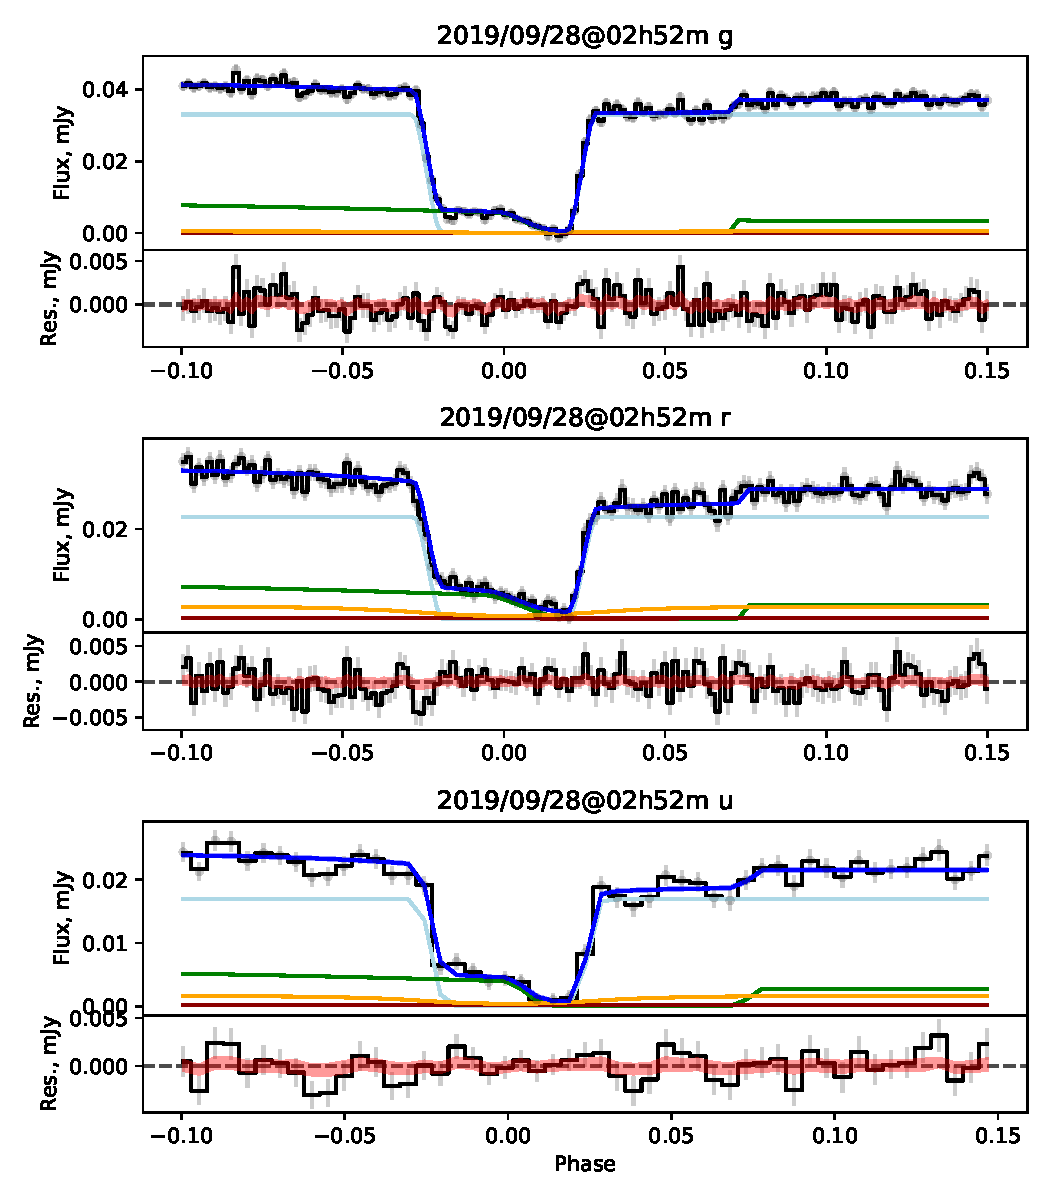
\includegraphics[width=\textwidth]{figures/results/three_cvs_with_weird_colours/ASASSN-17jf/ASASSN-17jf_1.pdf}
    \caption{ASASSN-17jf lightcurve models. {\it Top}:~{\bf grey points} are the observed flux, and note that the photometric system is the SDSS as per \S\ref{sect:observations:flux calibrating the lightcurve}; {\bf black line} is the observed flux, with the mean Gaussian process sample subtracted; the {\bf dark blue line} is the mean lightcurve model, and the {\bf blue band} is the standard deviation on this in the MCMC chain. The components of the model are also shown: the {\bf light blue line} is the white dwarf flux, {\bf green line} is the bright spot, {\bf orange line} is the disc, and the {\bf red line} is the donor. {\it Bottom}:~The residuals between the data and model are plotted as the {\bf black line}, with grey error bars. The Gaussian process 1-sigma region is shown as a {\bf red band}.}
    \label{fig:ASASSN-17jf all lightcurves}
\end{figure}
\begin{figure}
    \centering
    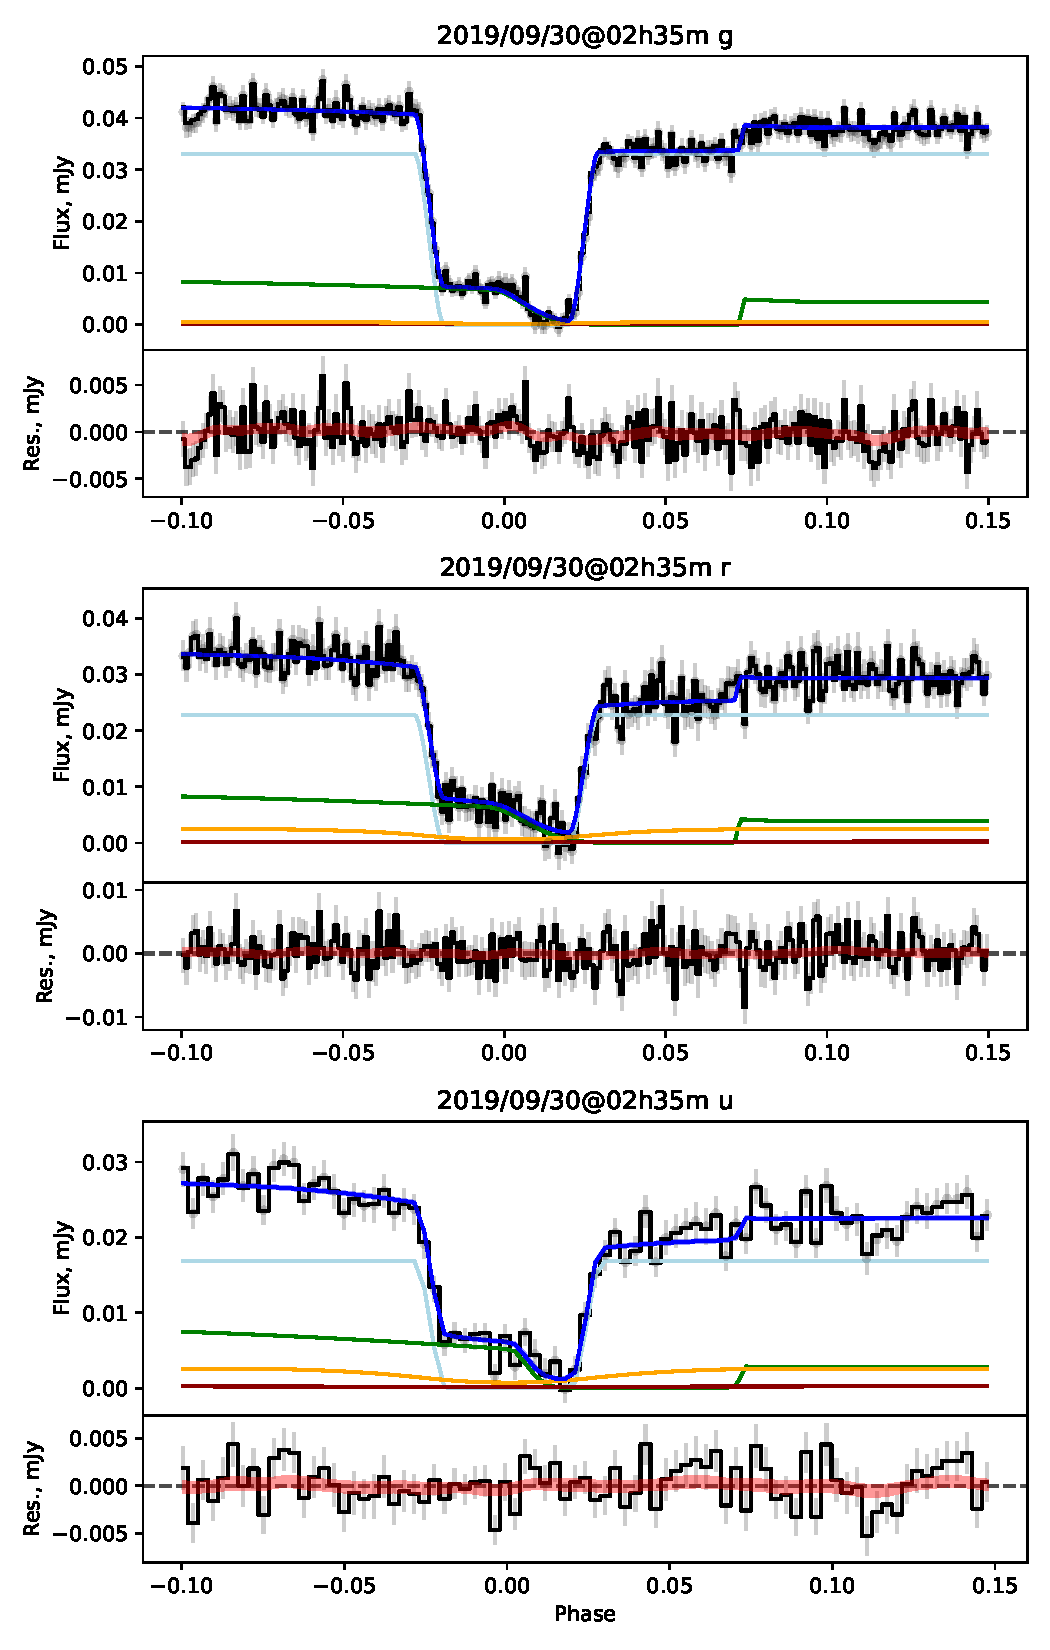
\includegraphics[width=\textwidth]{figures/results/three_cvs_with_weird_colours/ASASSN-17jf/ASASSN-17jf_2.pdf}
    \caption{ASASSN-17jf lightcurve models (cont.)}
    \label{fig:ASASSN-17jf all lightcurves cont 1}
\end{figure}
\begin{figure}
    \centering
    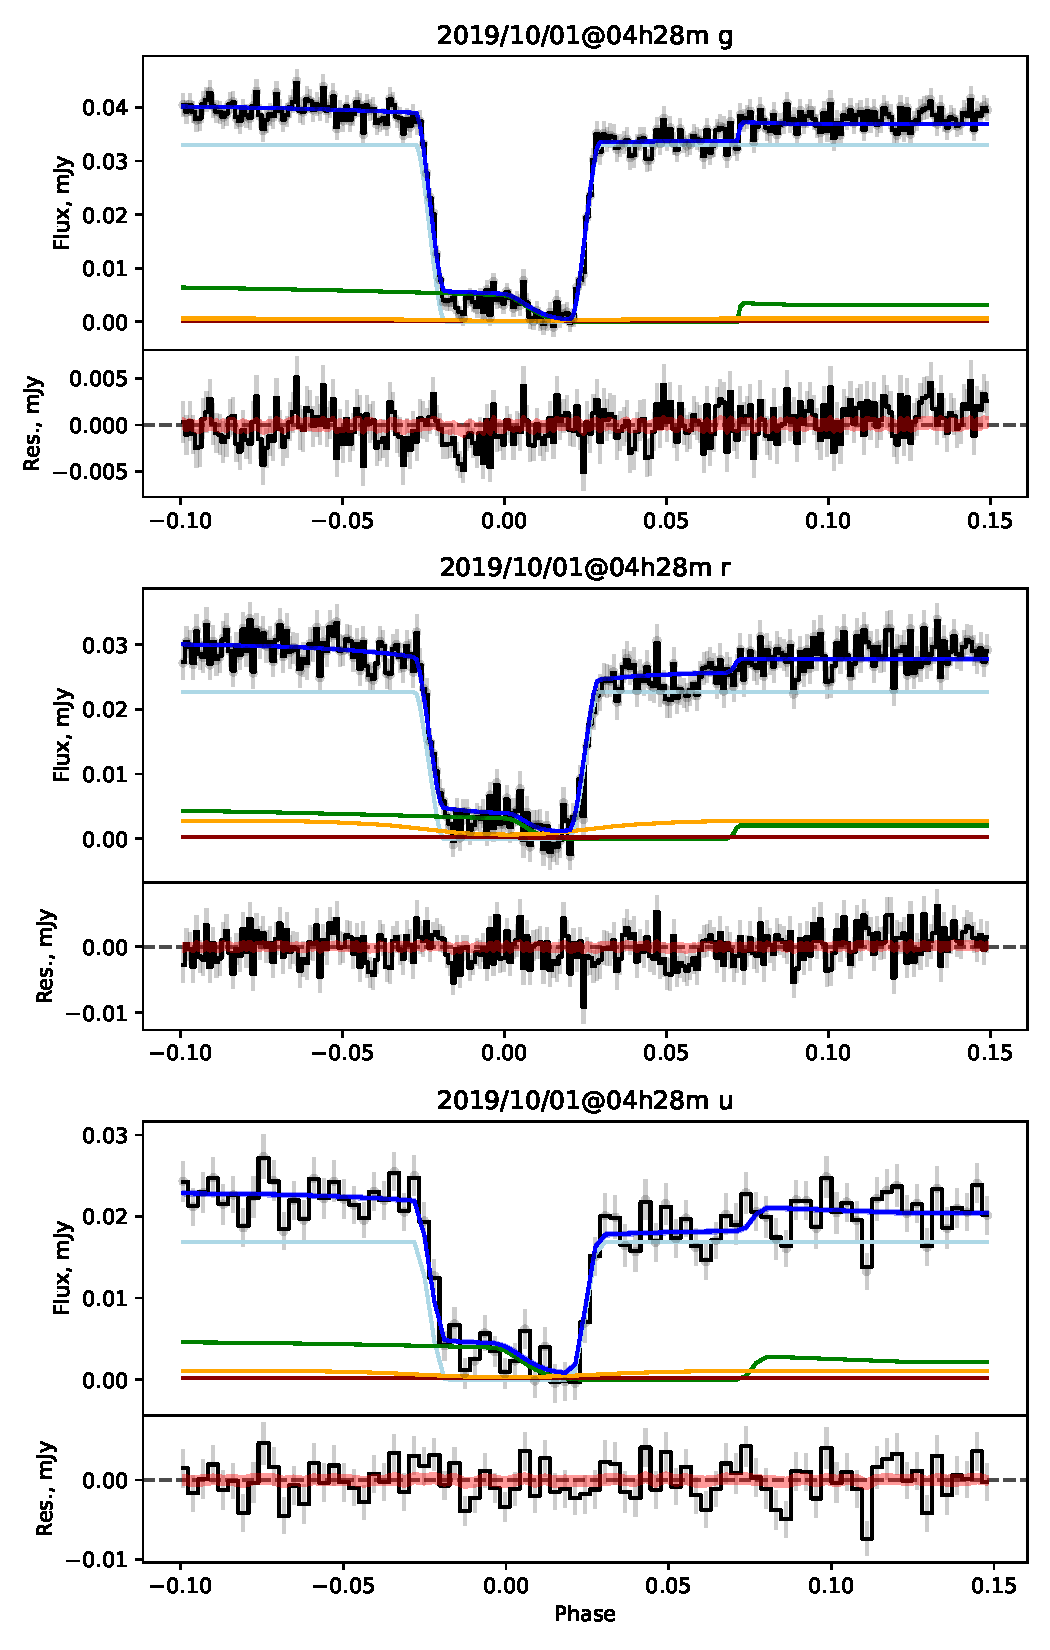
\includegraphics[width=\textwidth]{figures/results/three_cvs_with_weird_colours/ASASSN-17jf/ASASSN-17jf_3.pdf}
    \caption{ASASSN-17jf lightcurve models (cont.)}
    \label{fig:ASASSN-17jf all lightcurves cont 2}
\end{figure}



\begin{figure}
    \centering
    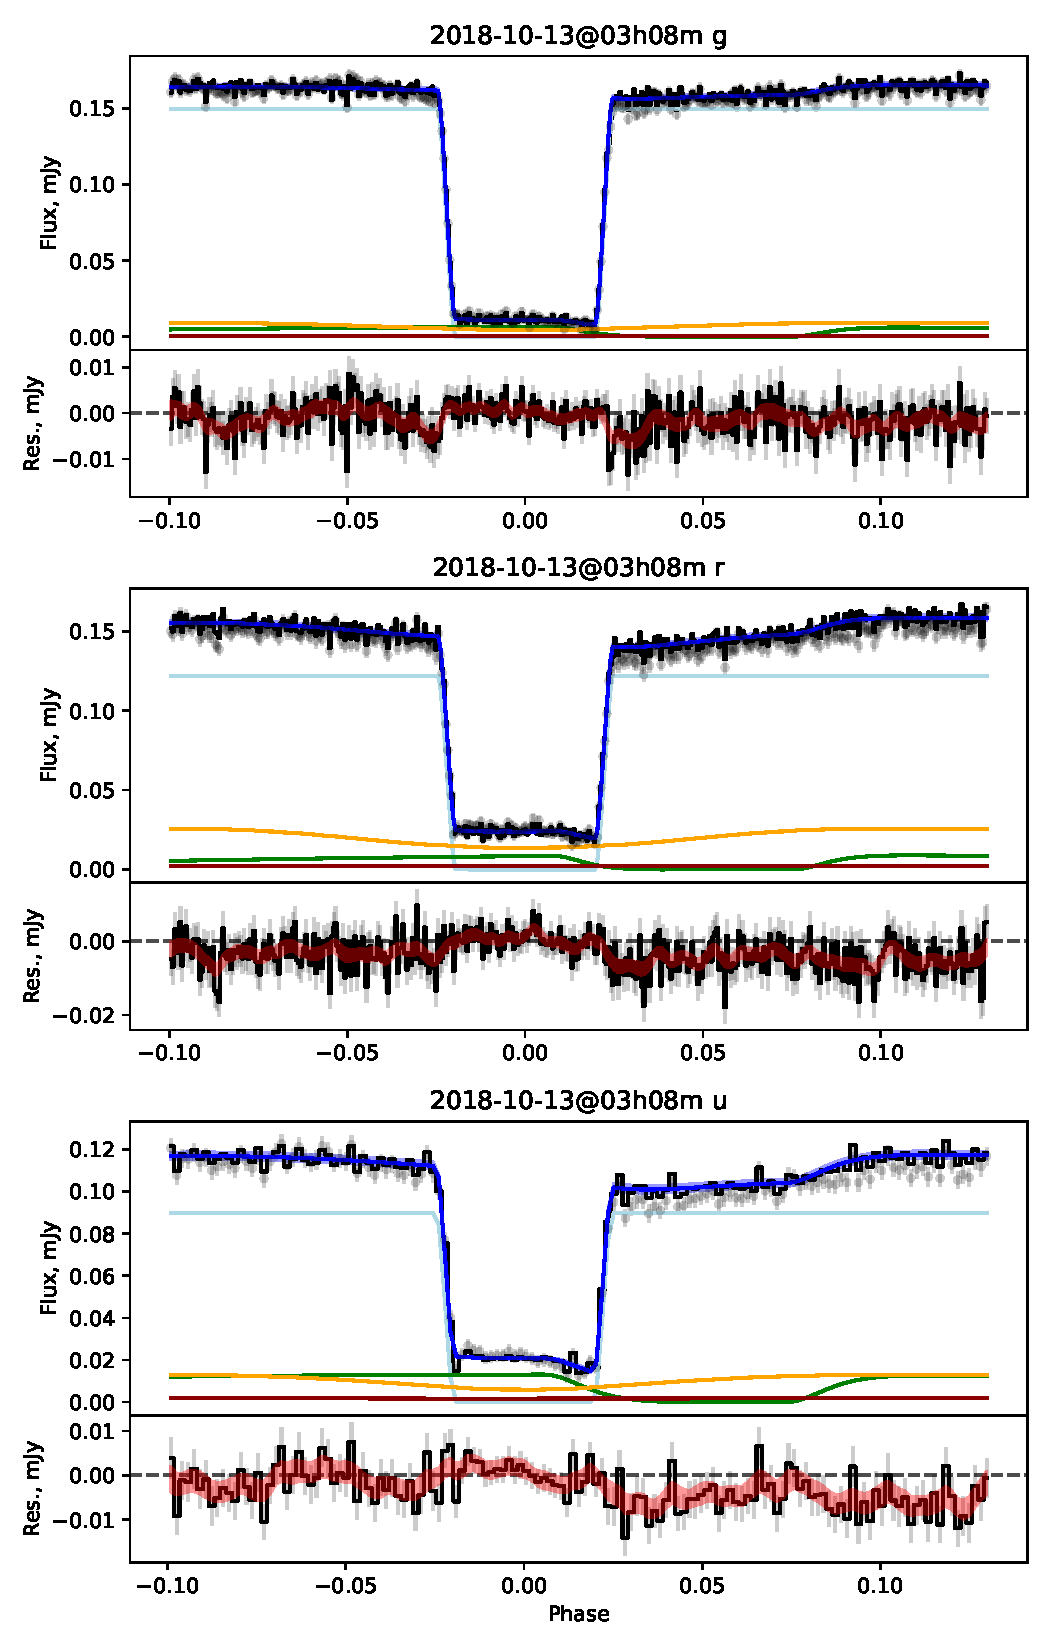
\includegraphics[width=\textwidth]{figures/results/three_cvs_with_weird_colours/ASASSN-16kr/ASASSN-16kr_1.pdf}
    \caption{ASASSN-16kr lightcurve models. Symbols are the same as Figure~\ref{fig:ASASSN-17jf all lightcurves}}
    \label{fig:ASASSN-16kr all lightcurves}
\end{figure}
\begin{figure}
    \centering
    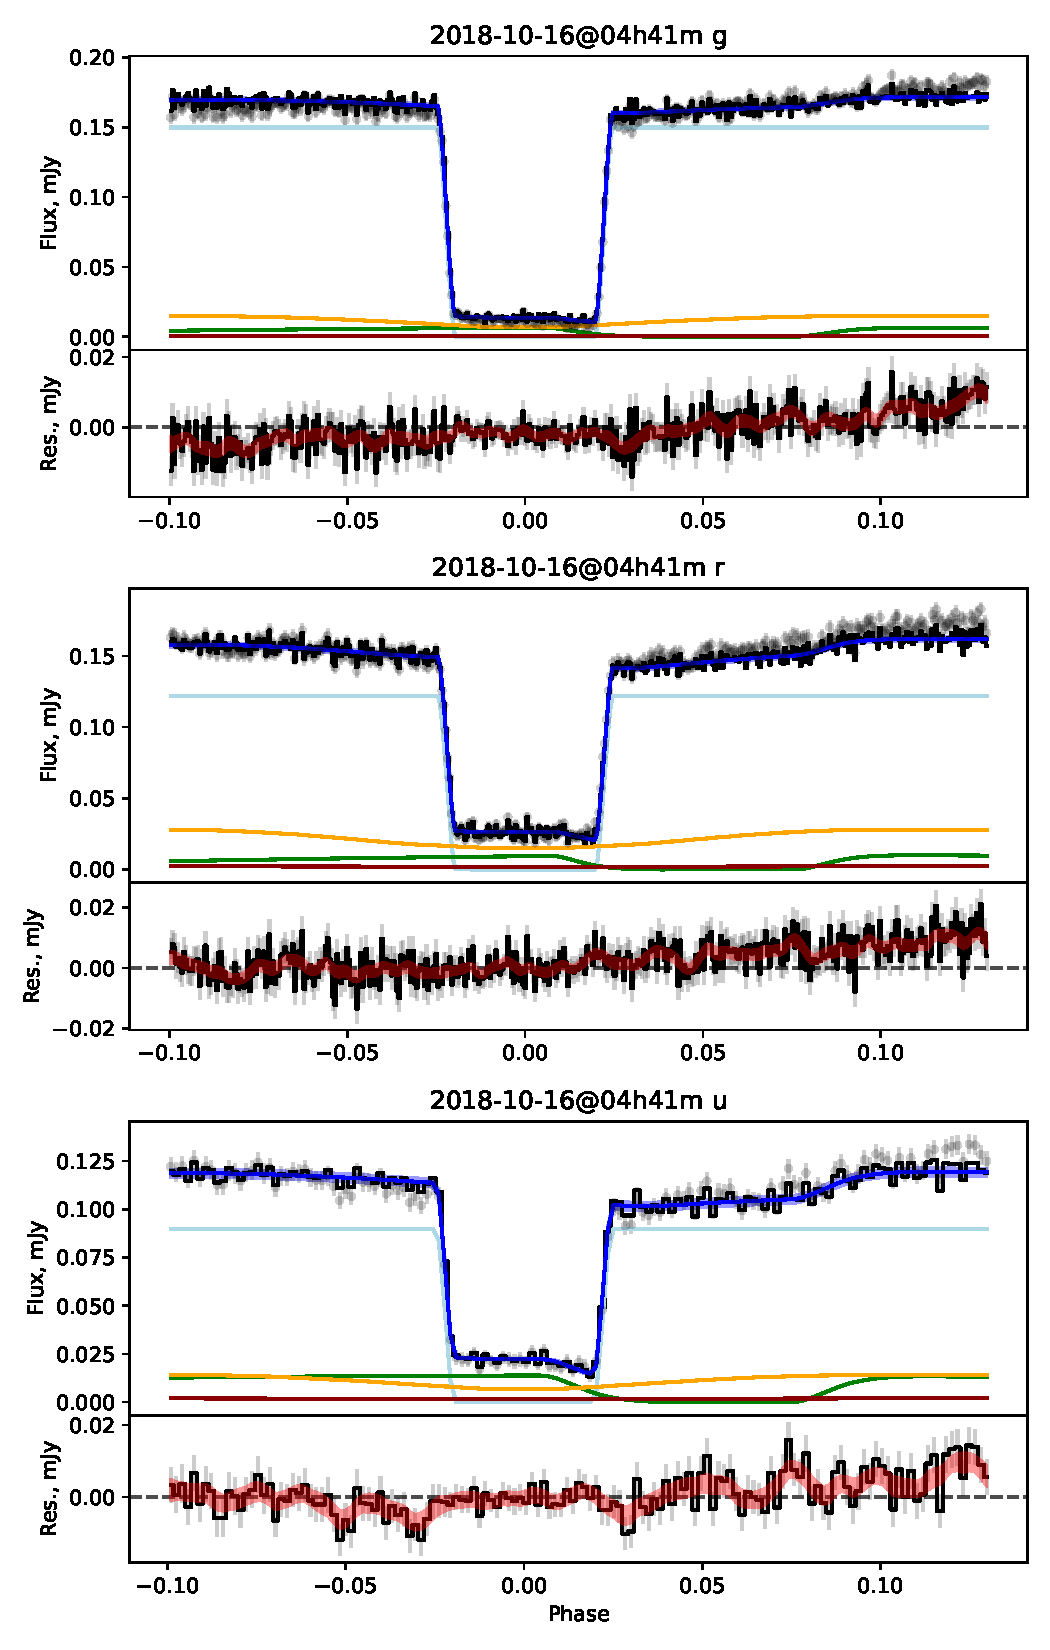
\includegraphics[width=\textwidth]{figures/results/three_cvs_with_weird_colours/ASASSN-16kr/ASASSN-16kr_2.pdf}
    \caption{ASASSN-16kr lightcurve models (cont.)}
    \label{fig:ASASSN-16kr all lightcurves cont 1}
\end{figure}
\begin{figure}
    \centering
    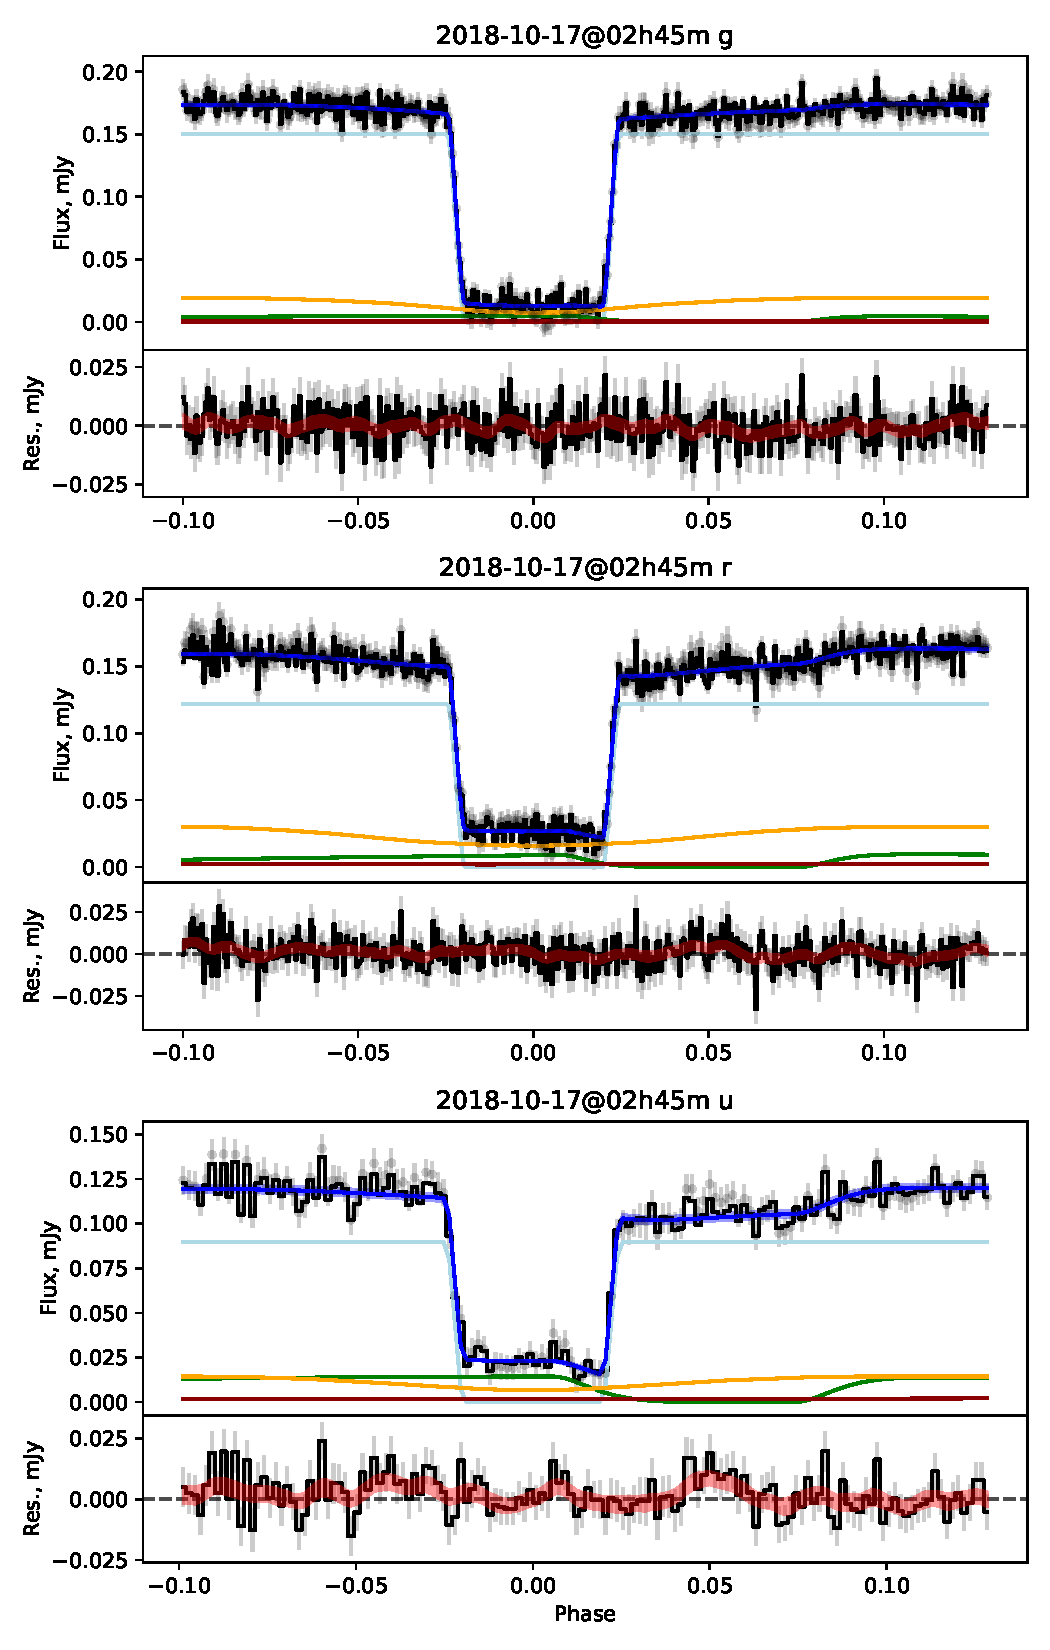
\includegraphics[width=\textwidth]{figures/results/three_cvs_with_weird_colours/ASASSN-16kr/ASASSN-16kr_3.pdf}
    \caption{ASASSN-16kr lightcurve models (cont.)}
    \label{fig:ASASSN-16kr all lightcurves cont 2}
\end{figure}
\begin{figure}
    \centering
    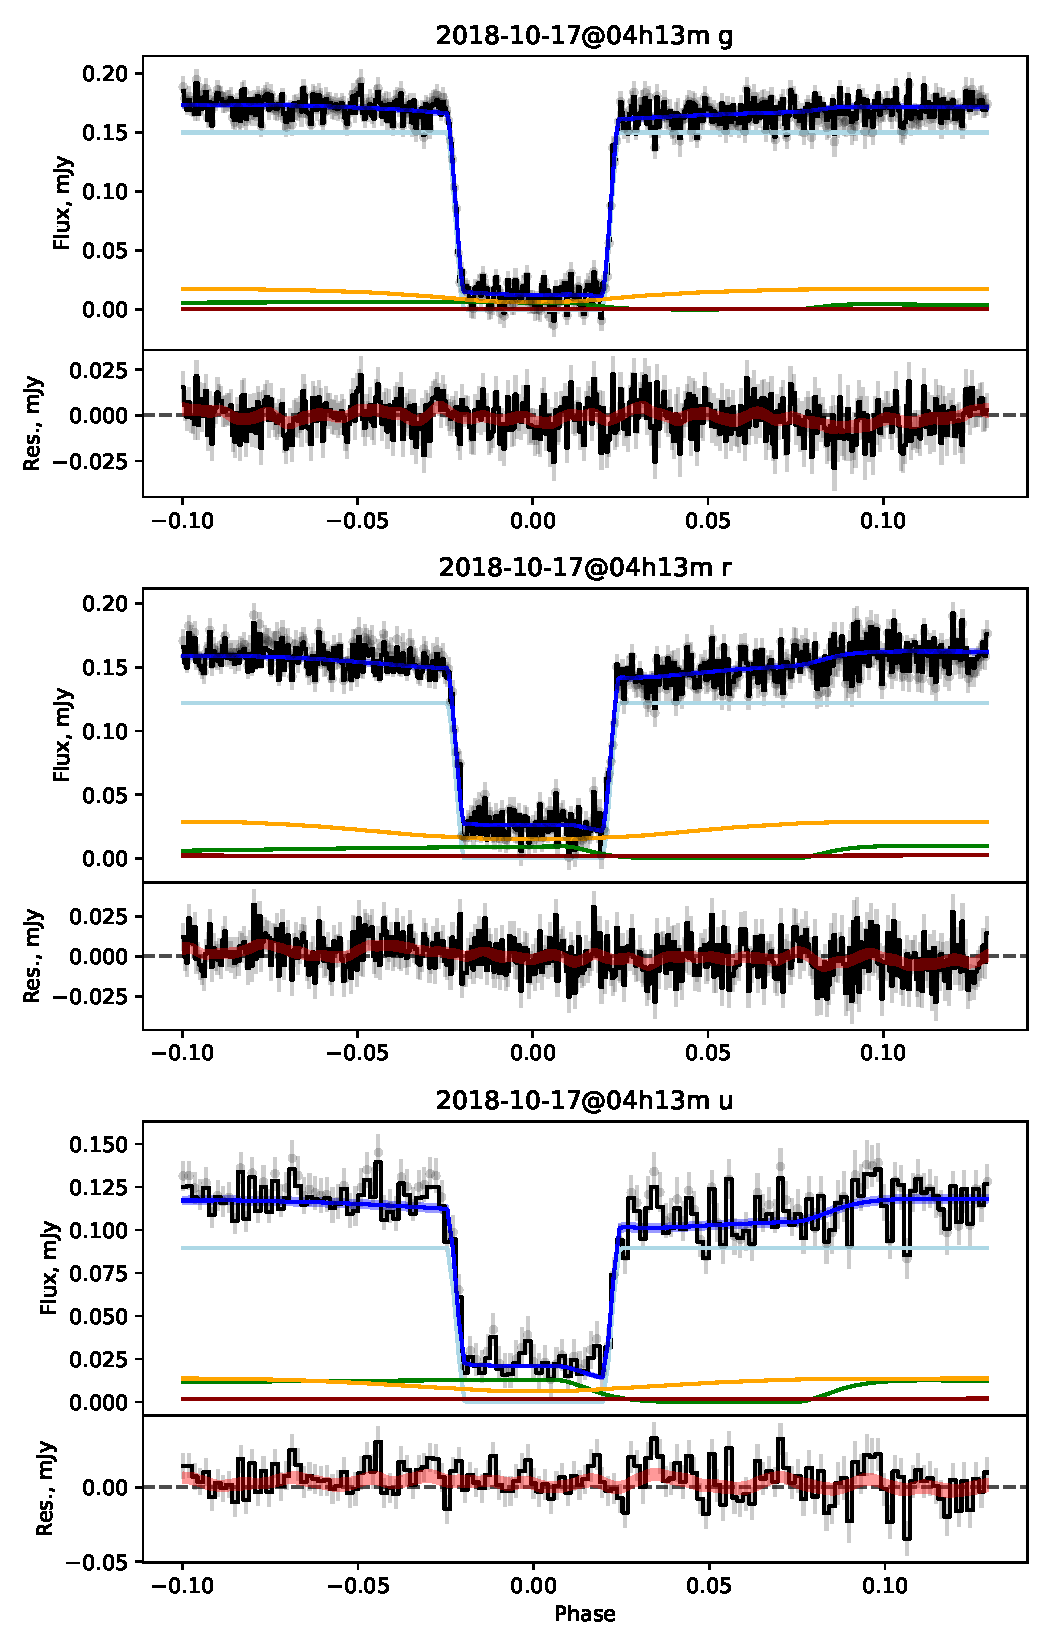
\includegraphics[width=\textwidth]{figures/results/three_cvs_with_weird_colours/ASASSN-16kr/ASASSN-16kr_4.pdf}
    \caption{ASASSN-16kr lightcurve models (cont.)}
    \label{fig:ASASSN-16kr all lightcurves cont 3}
\end{figure}
\begin{figure}
    \centering
    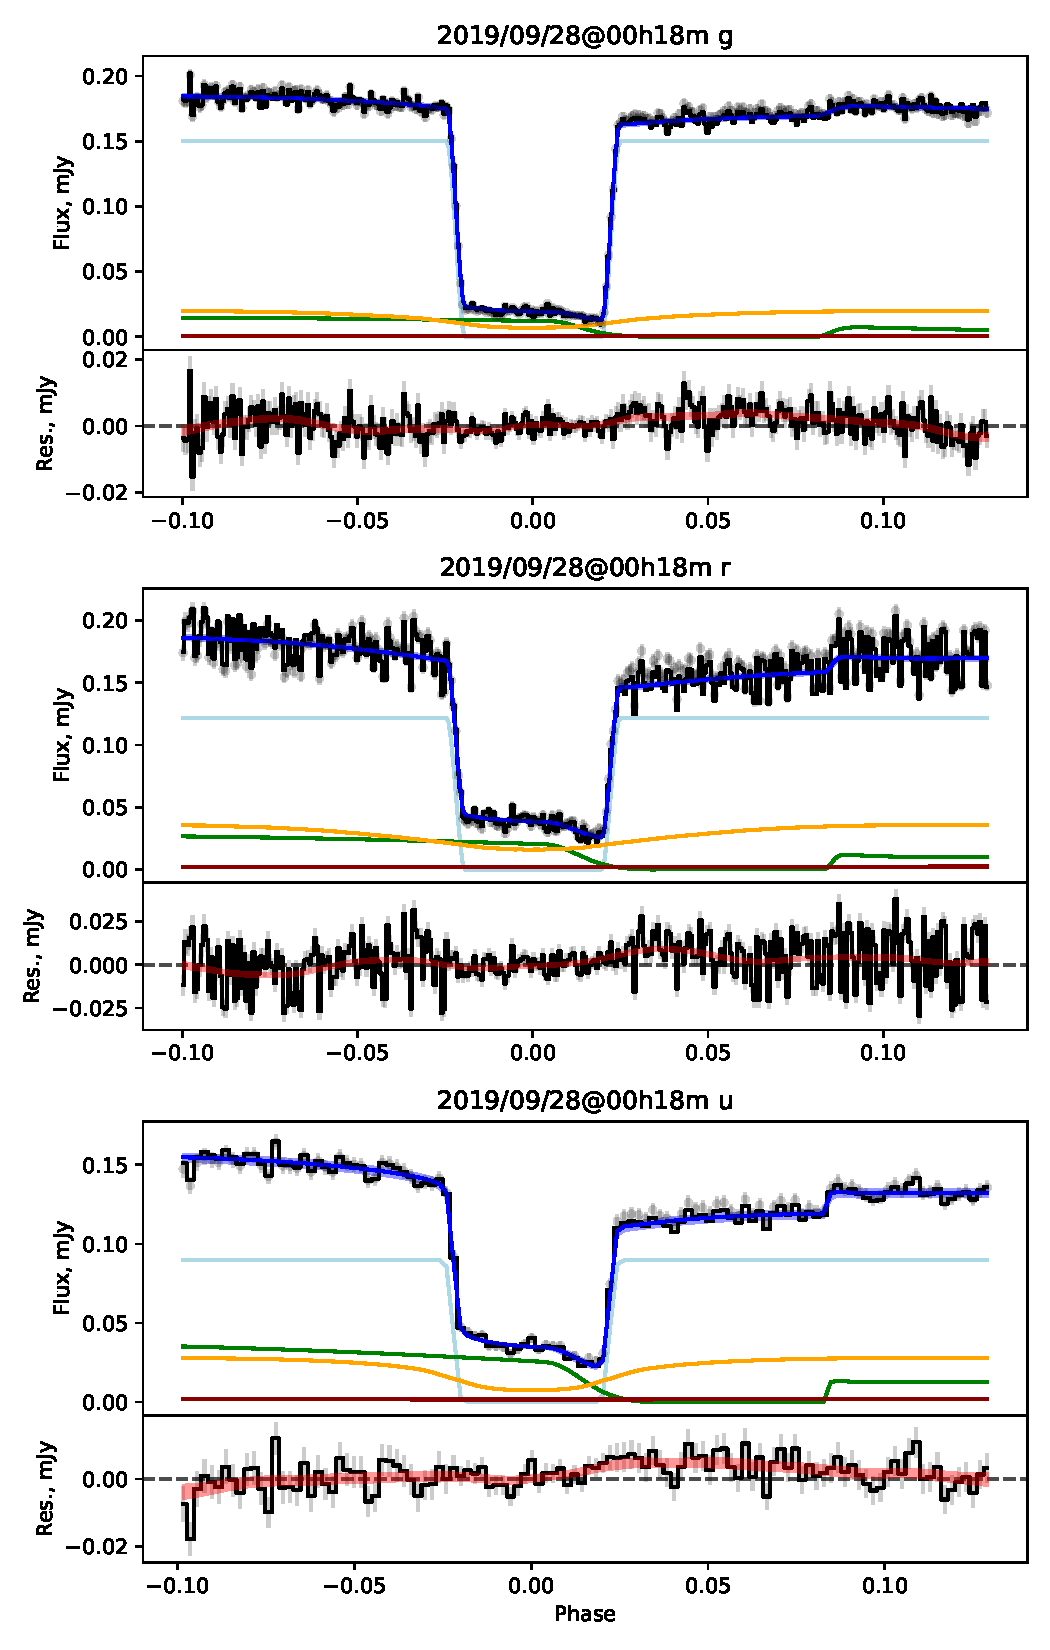
\includegraphics[width=\textwidth]{figures/results/three_cvs_with_weird_colours/ASASSN-16kr/ASASSN-16kr_5.pdf}
    \caption{ASASSN-16kr lightcurve models (cont.)}
    \label{fig:ASASSN-16kr all lightcurves cont 4}
\end{figure}
\begin{figure}
    \centering
    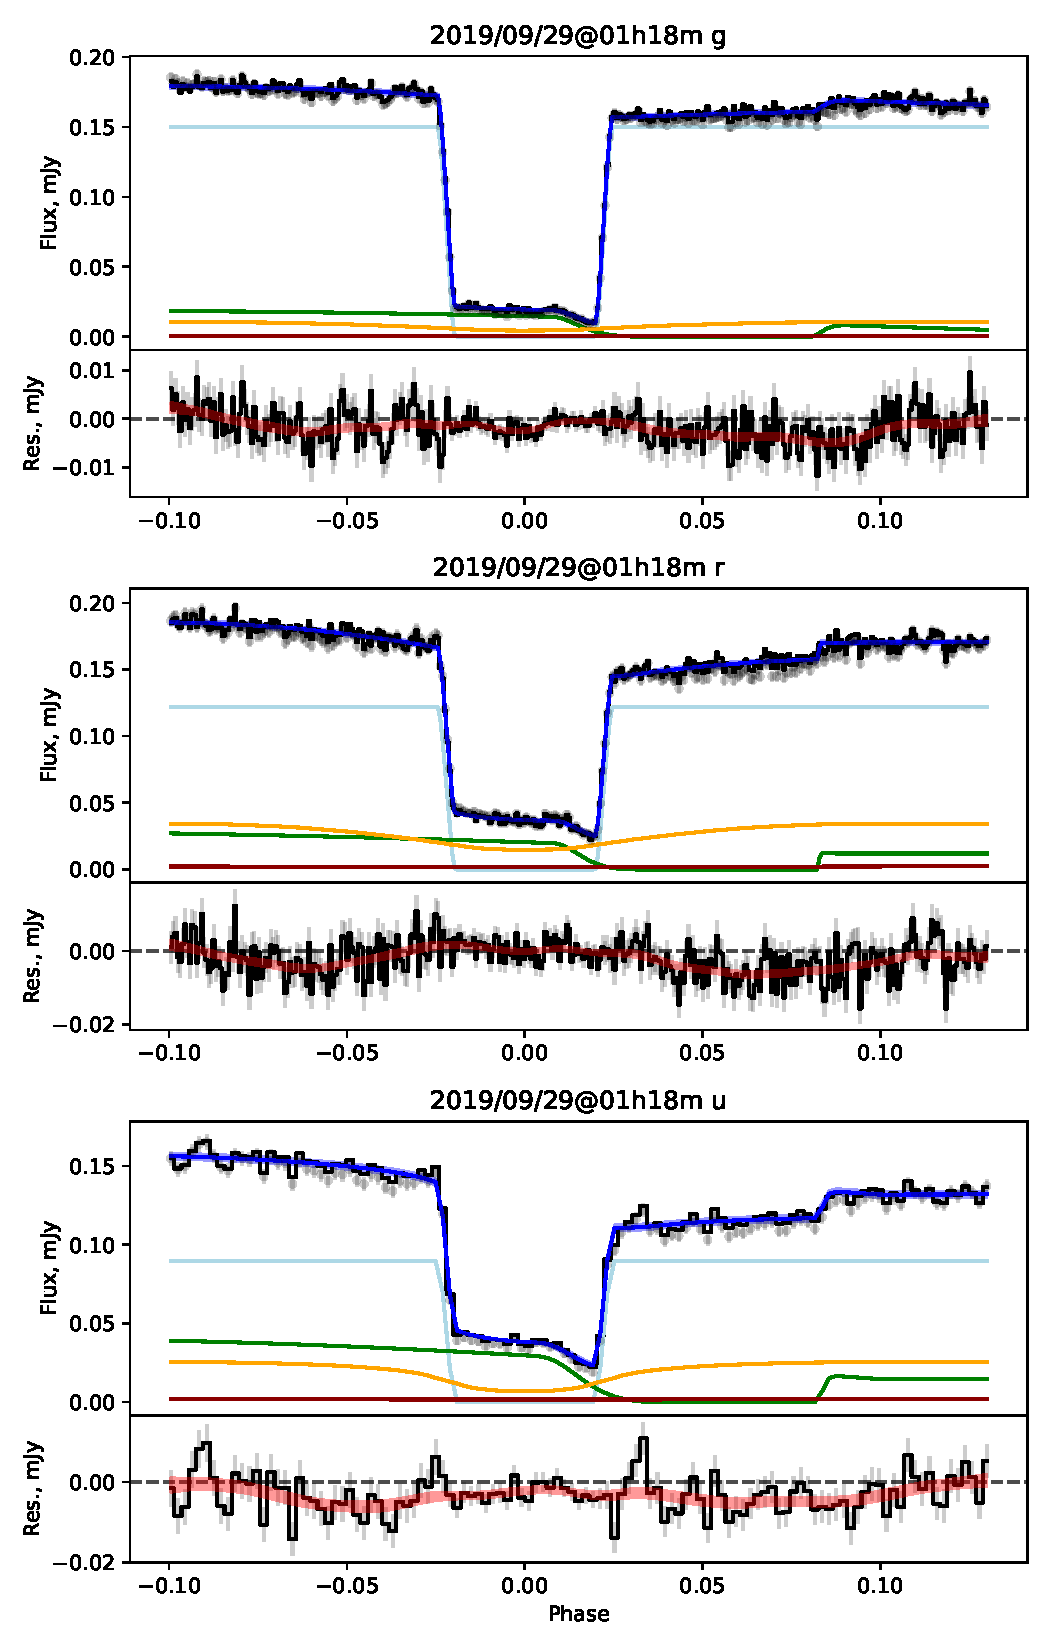
\includegraphics[width=\textwidth]{figures/results/three_cvs_with_weird_colours/ASASSN-16kr/ASASSN-16kr_6.pdf}
    \caption{ASASSN-16kr lightcurve models (cont.)}
    \label{fig:ASASSN-16kr all lightcurves cont 5}
\end{figure}
\begin{figure}
    \centering
    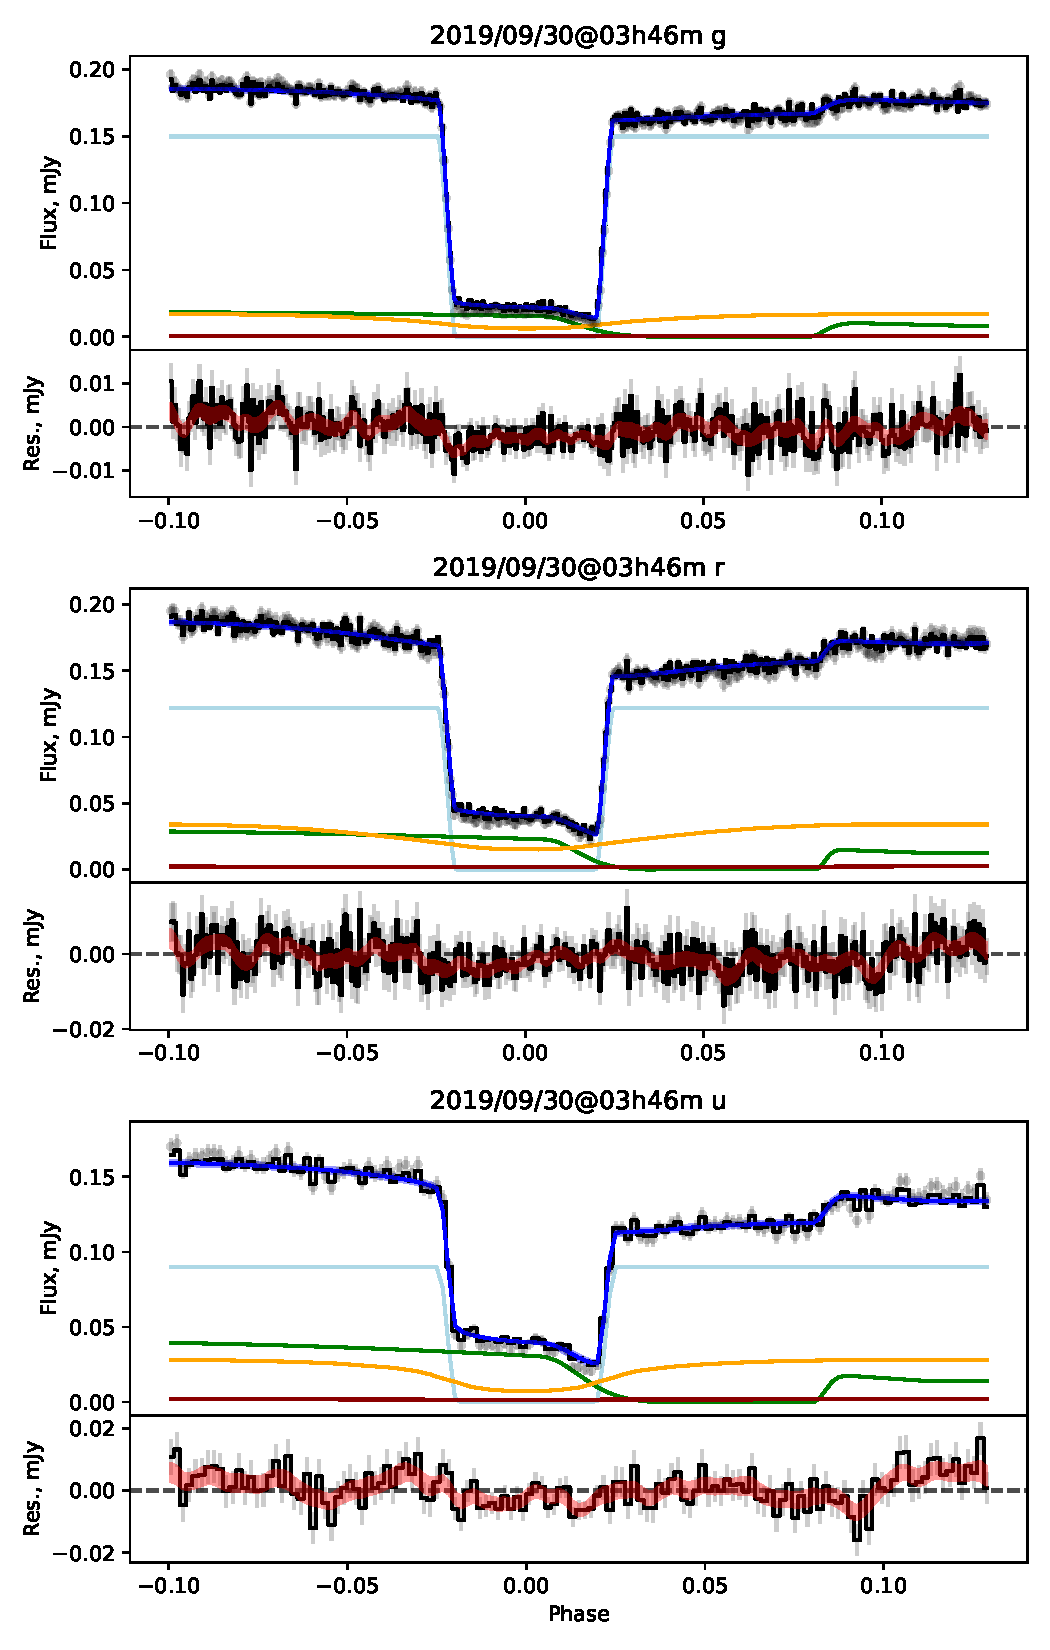
\includegraphics[width=\textwidth]{figures/results/three_cvs_with_weird_colours/ASASSN-16kr/ASASSN-16kr_7.pdf}
    \caption{ASASSN-16kr lightcurve models (cont.)}
    \label{fig:ASASSN-16kr all lightcurves cont 6}
\end{figure}



\begin{figure}
    \centering
    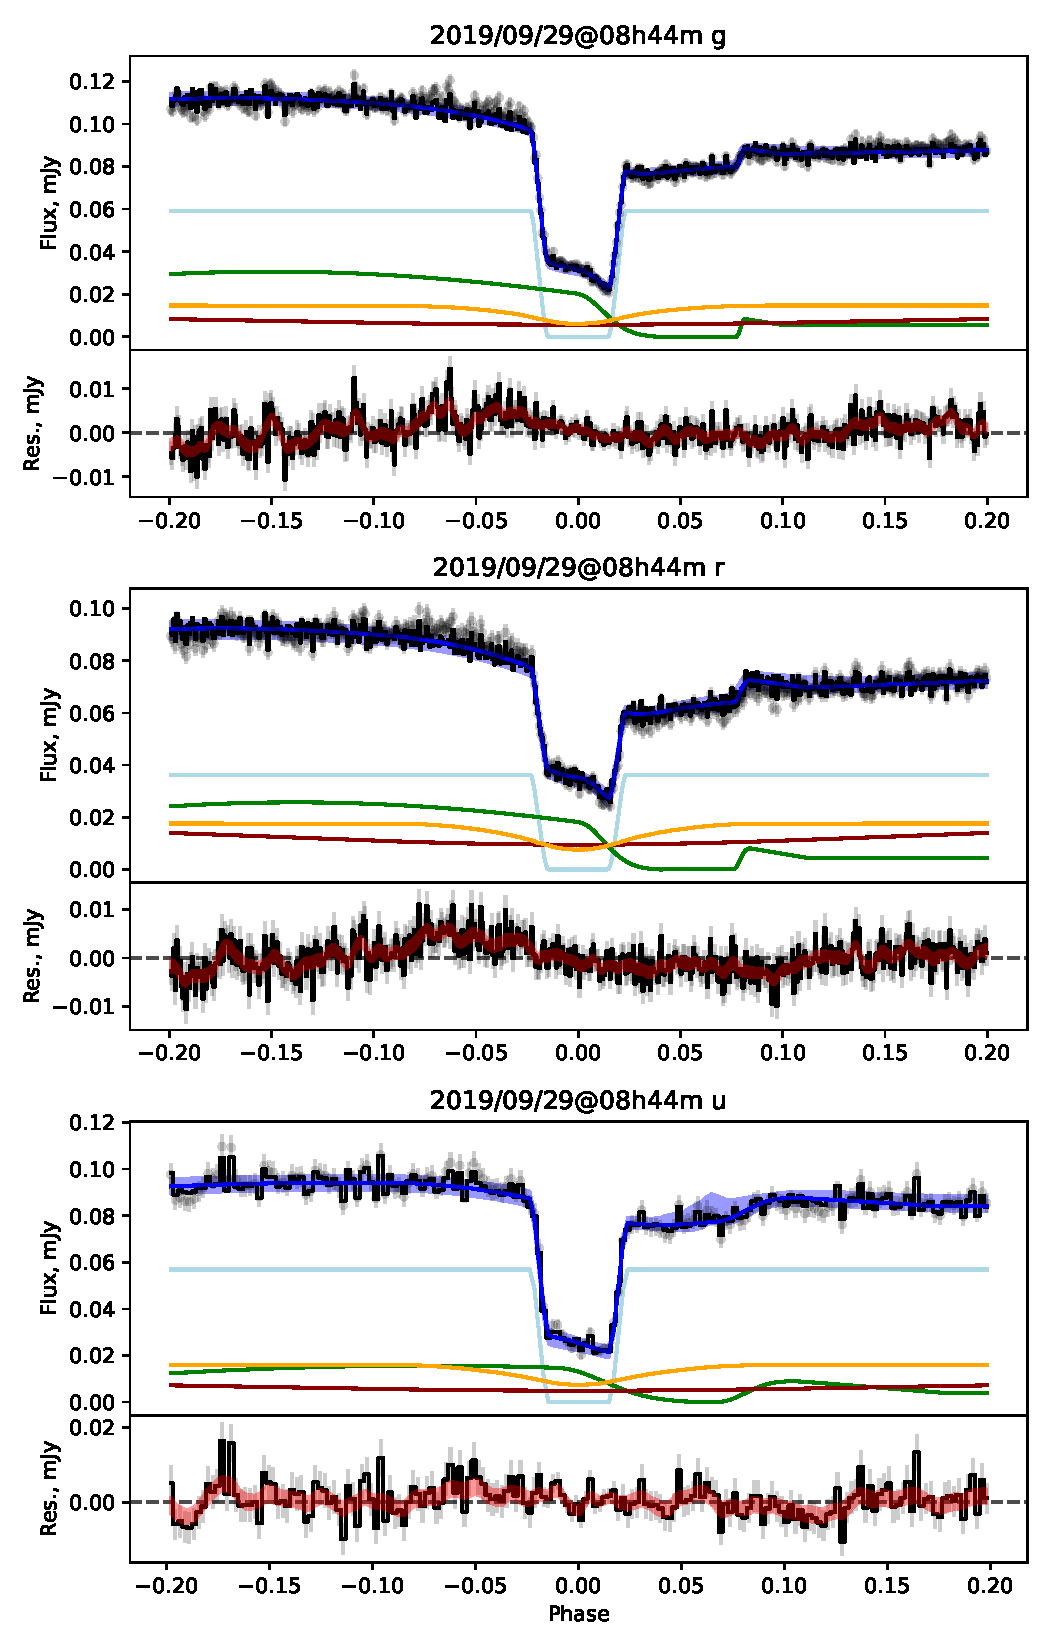
\includegraphics[width=\textwidth]{figures/results/three_cvs_with_weird_colours/SSS111126/SSS111126_1.pdf}
    \caption{SSSJ0522-3505 lightcurve models. Symbols are the same as Figure~\ref{fig:ASASSN-17jf all lightcurves}}
    \label{fig:SSSJ0522-3505 all lightcurves}
\end{figure}
\begin{figure}
    \centering
    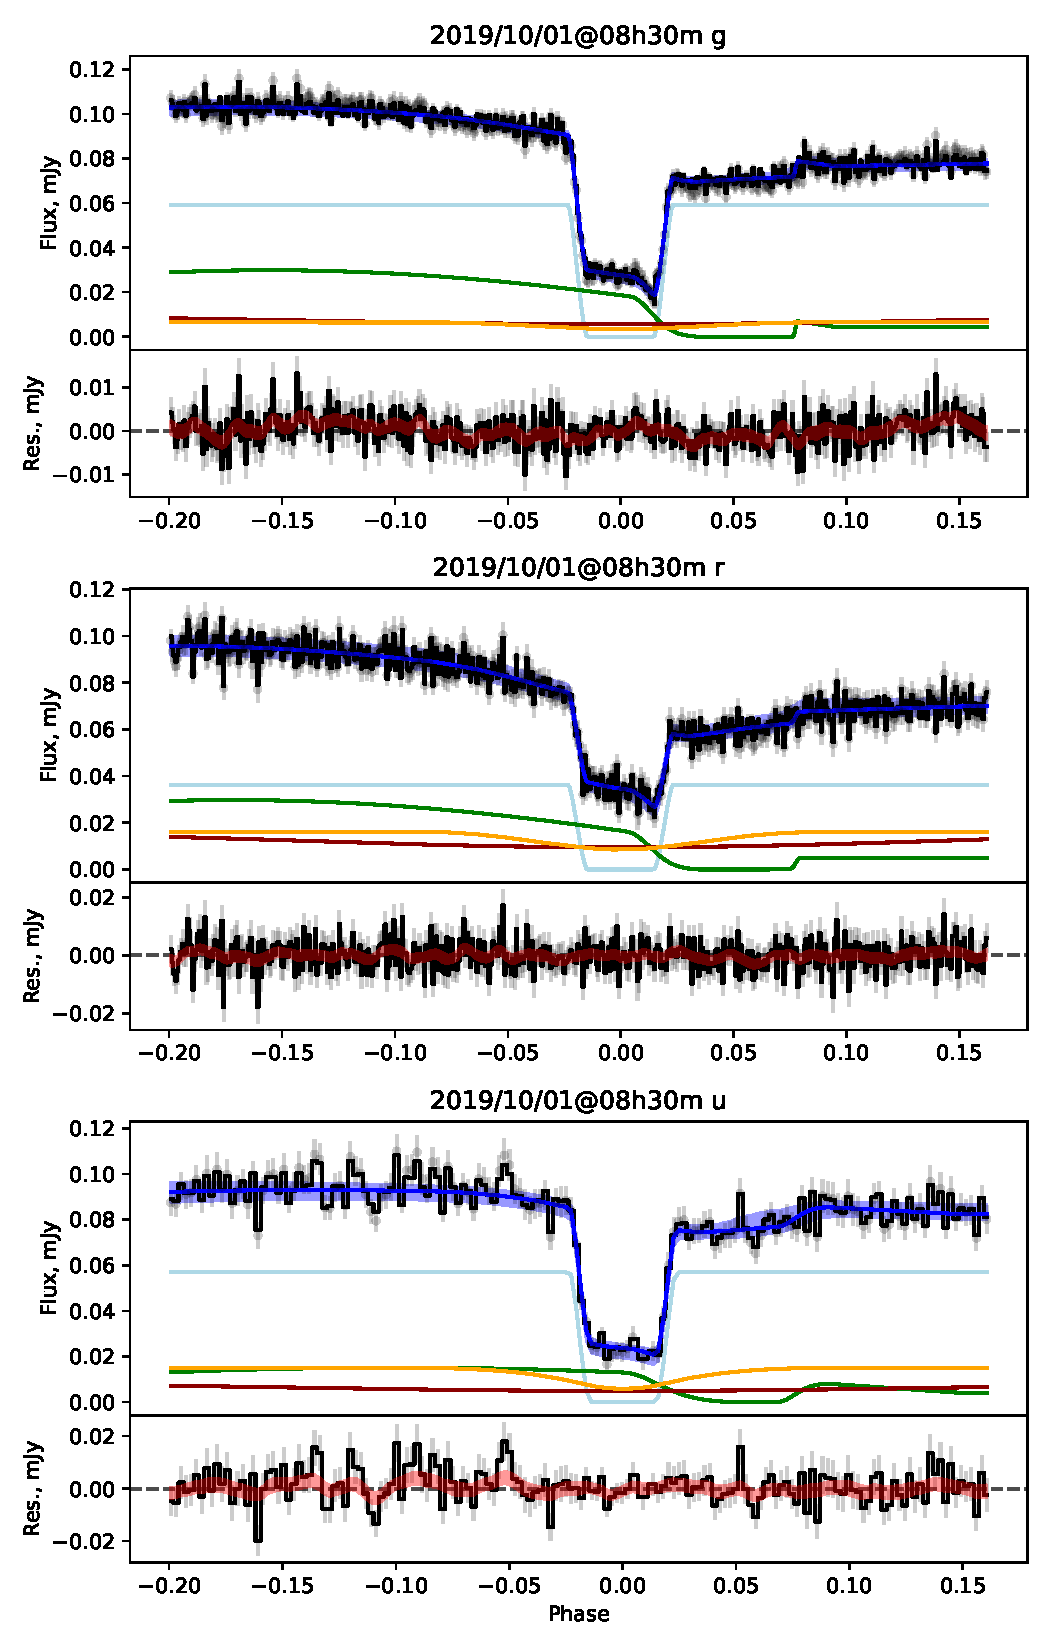
\includegraphics[width=\textwidth]{figures/results/three_cvs_with_weird_colours/SSS111126/SSS111126_2.pdf}
    \caption{SSSJ0522-3505 lightcurve models (cont.)}
    \label{fig:SSSJ0522-3505 all lightcurves cont 1}
\end{figure}
\begin{figure}
    \centering
    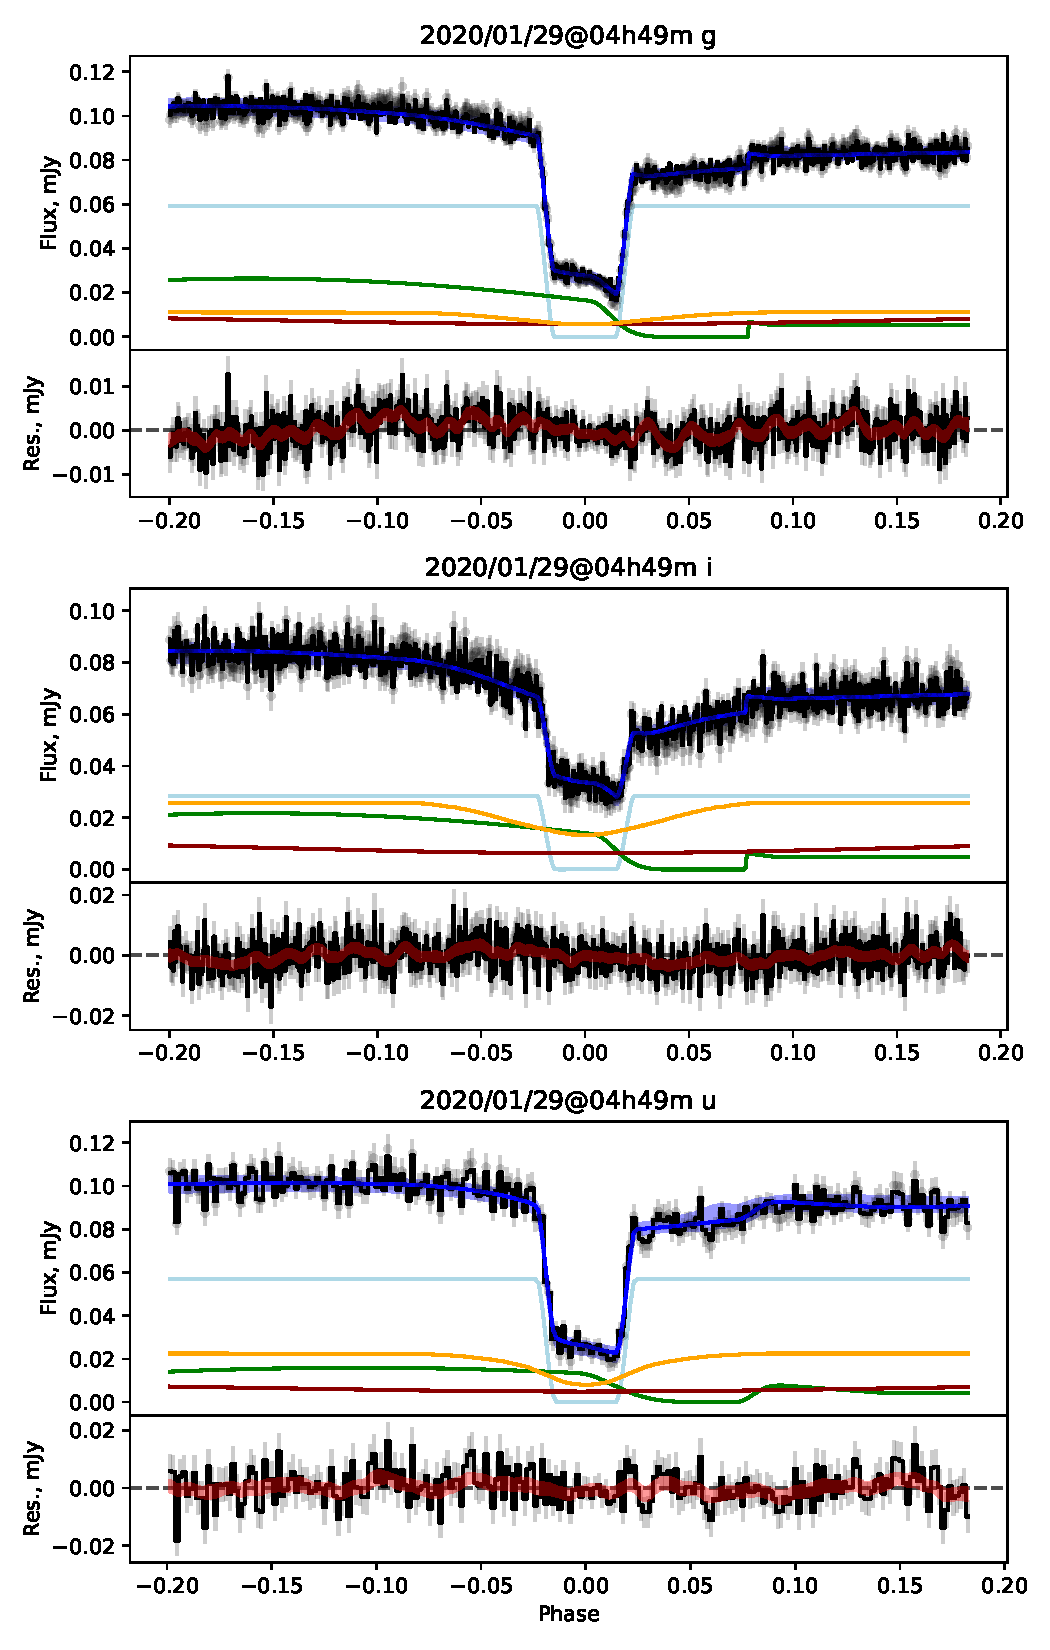
\includegraphics[width=\textwidth]{figures/results/three_cvs_with_weird_colours/SSS111126/SSS111126_3.pdf}
    \caption{SSSJ0522-3505 lightcurve models (cont.)}
    \label{fig:SSSJ0522-3505 all lightcurves cont 2}
\end{figure}



\begin{figure}
    \centering
    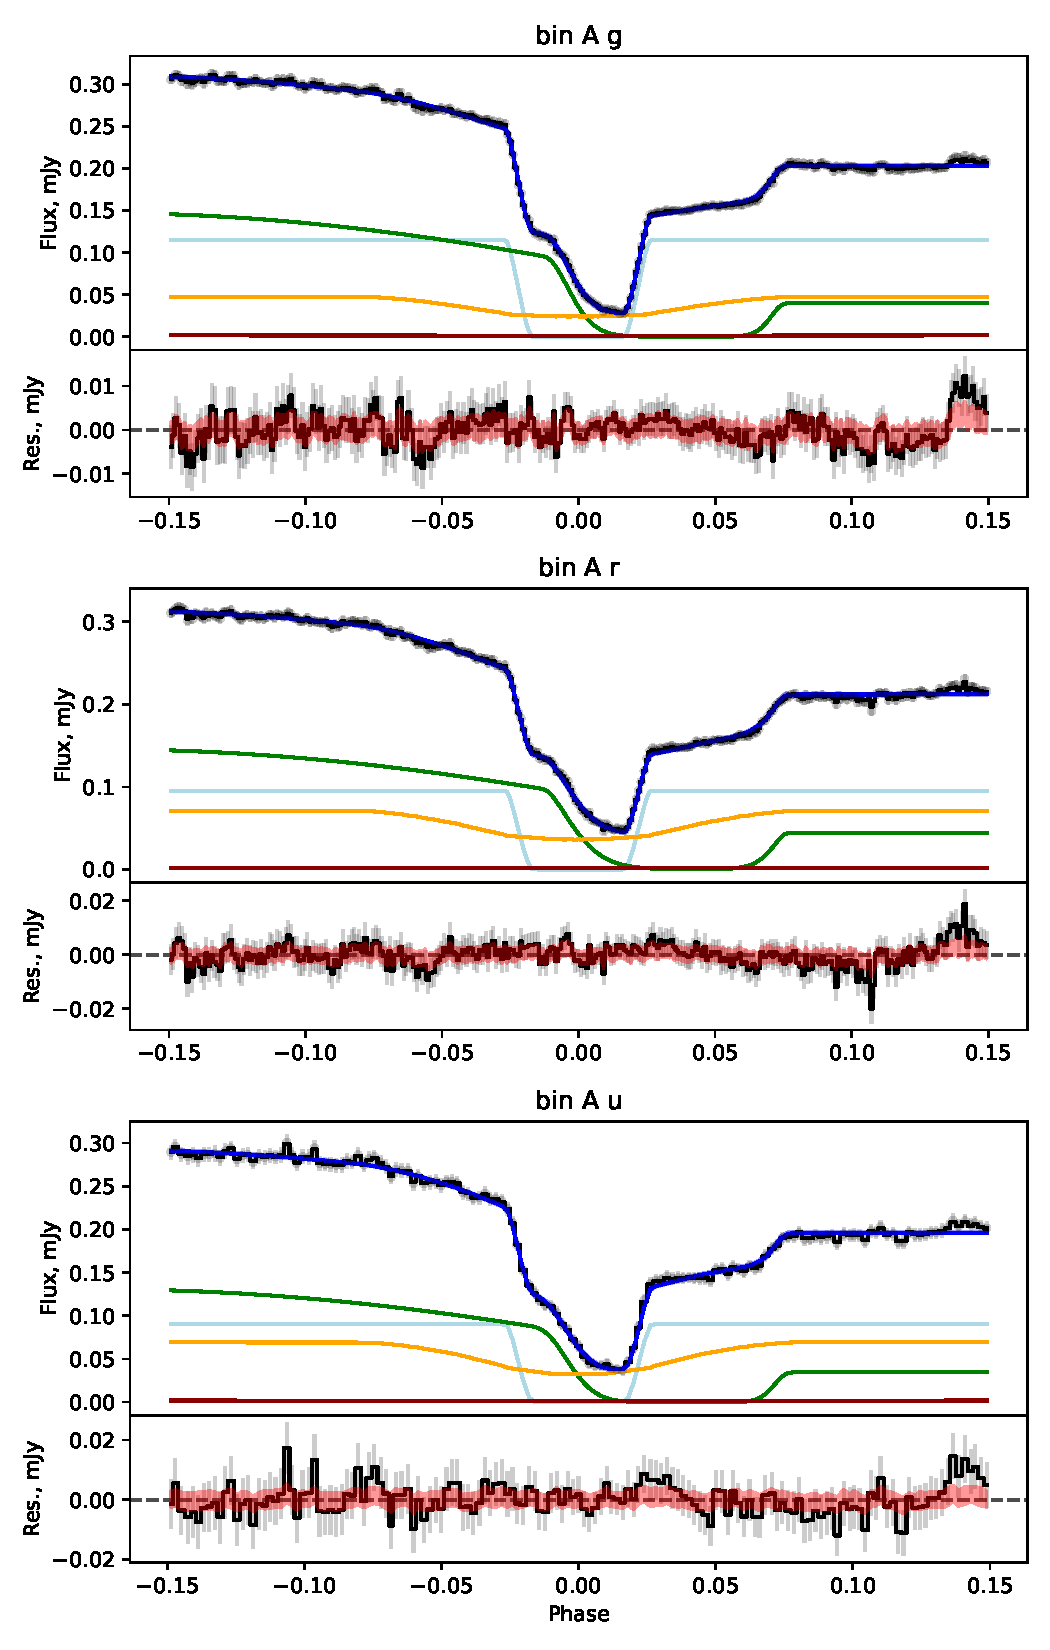
\includegraphics[width=\textwidth]{figures/results/ASASSN-14hq/ASASSN-14hq_1.pdf}
    \caption{ASASSN-14hq lightcurve models. Symbols are the same as Figure~\ref{fig:ASASSN-17jf all lightcurves}}
    \label{fig:ASASSN-14hq all lightcurves}
\end{figure}
\begin{figure}
    \centering
    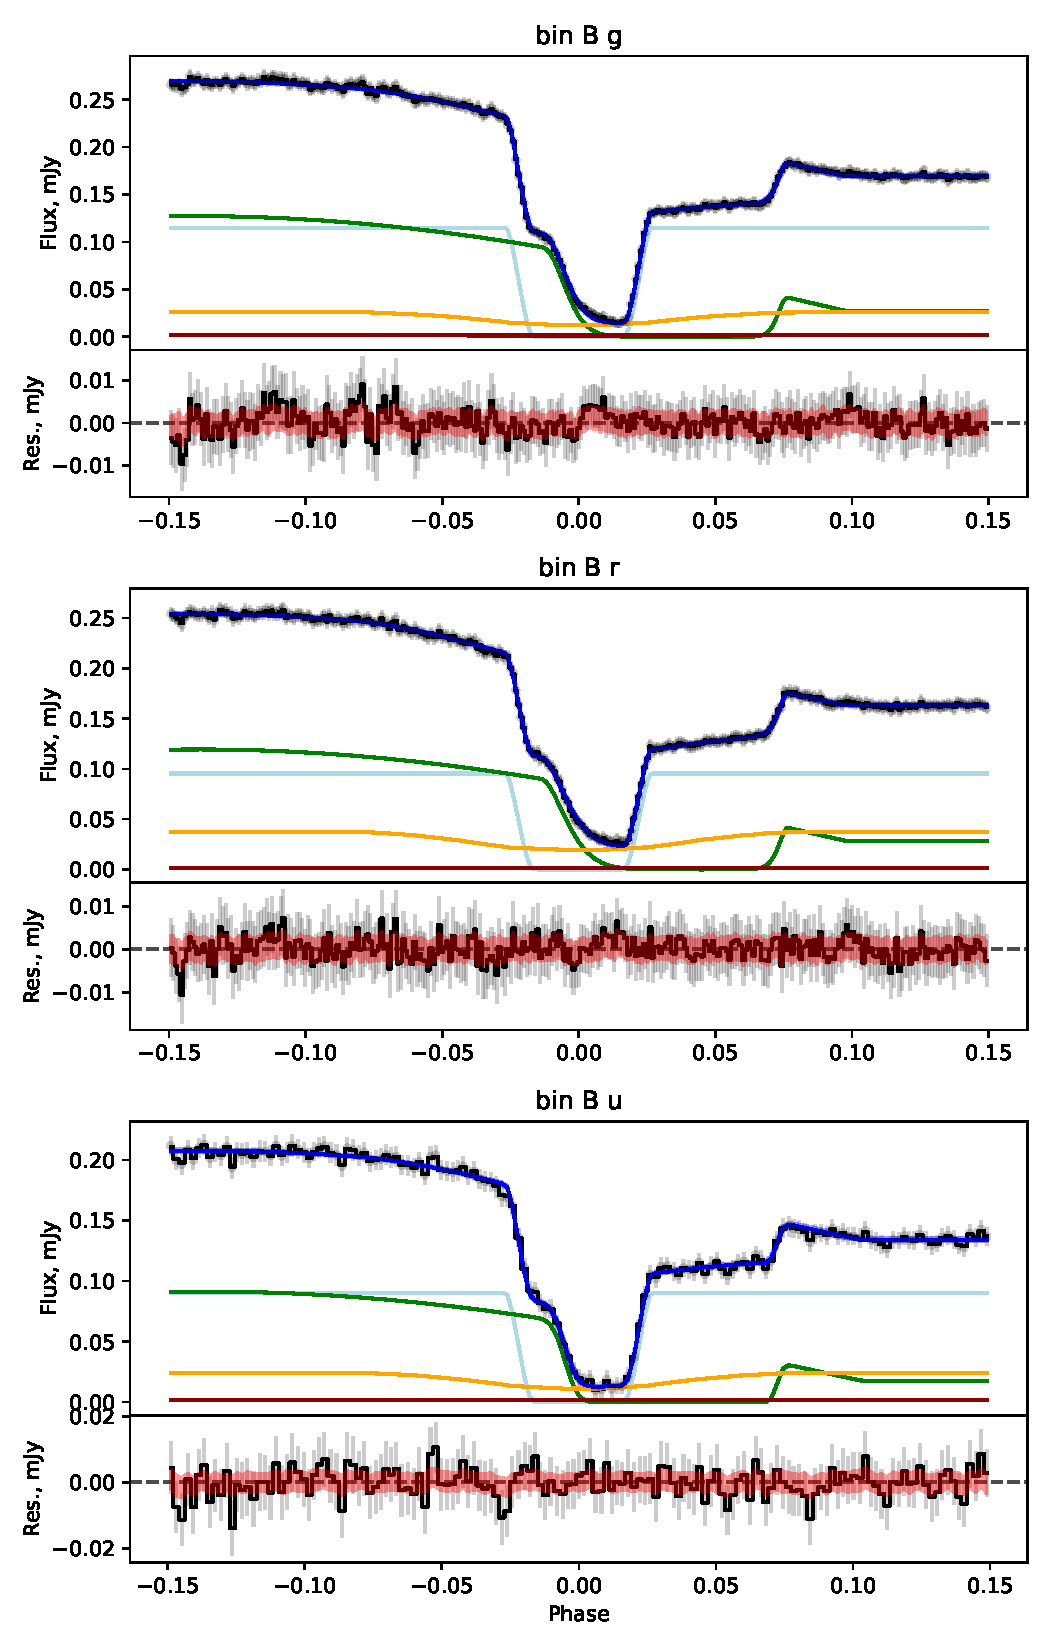
\includegraphics[width=\textwidth]{figures/results/ASASSN-14hq/ASASSN-14hq_2.pdf}
    \caption{ASASSN-14hq lightcurve models (cont.)}
    \label{fig:ASASSN-14hq all lightcurves cont}
\end{figure}



\begin{figure}
    \centering
    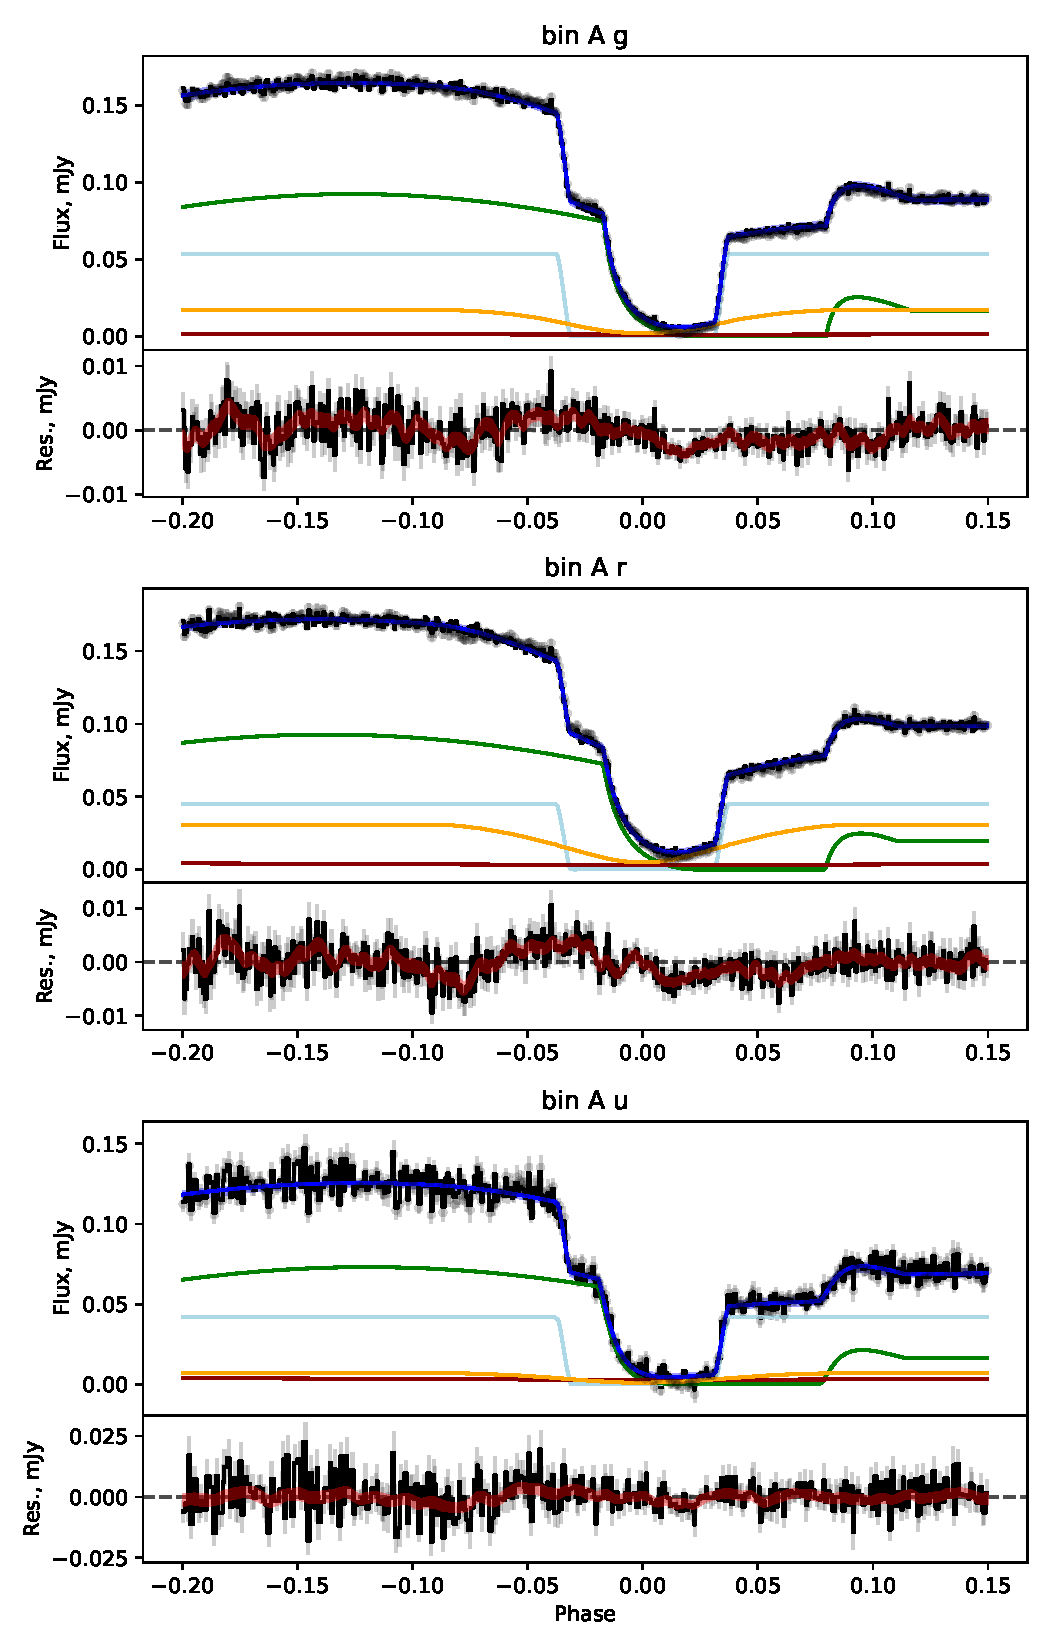
\includegraphics[width=\textwidth]{figures/results/ASASSN-14kb/ASASSN-14kb_1.pdf}
    \caption{ASASSN-14kb lightcurve models. Symbols are the same as Figure~\ref{fig:ASASSN-17jf all lightcurves}}
    \label{fig:ASASSN-14kb all lightcurves}
\end{figure}



\begin{figure}
    \centering
    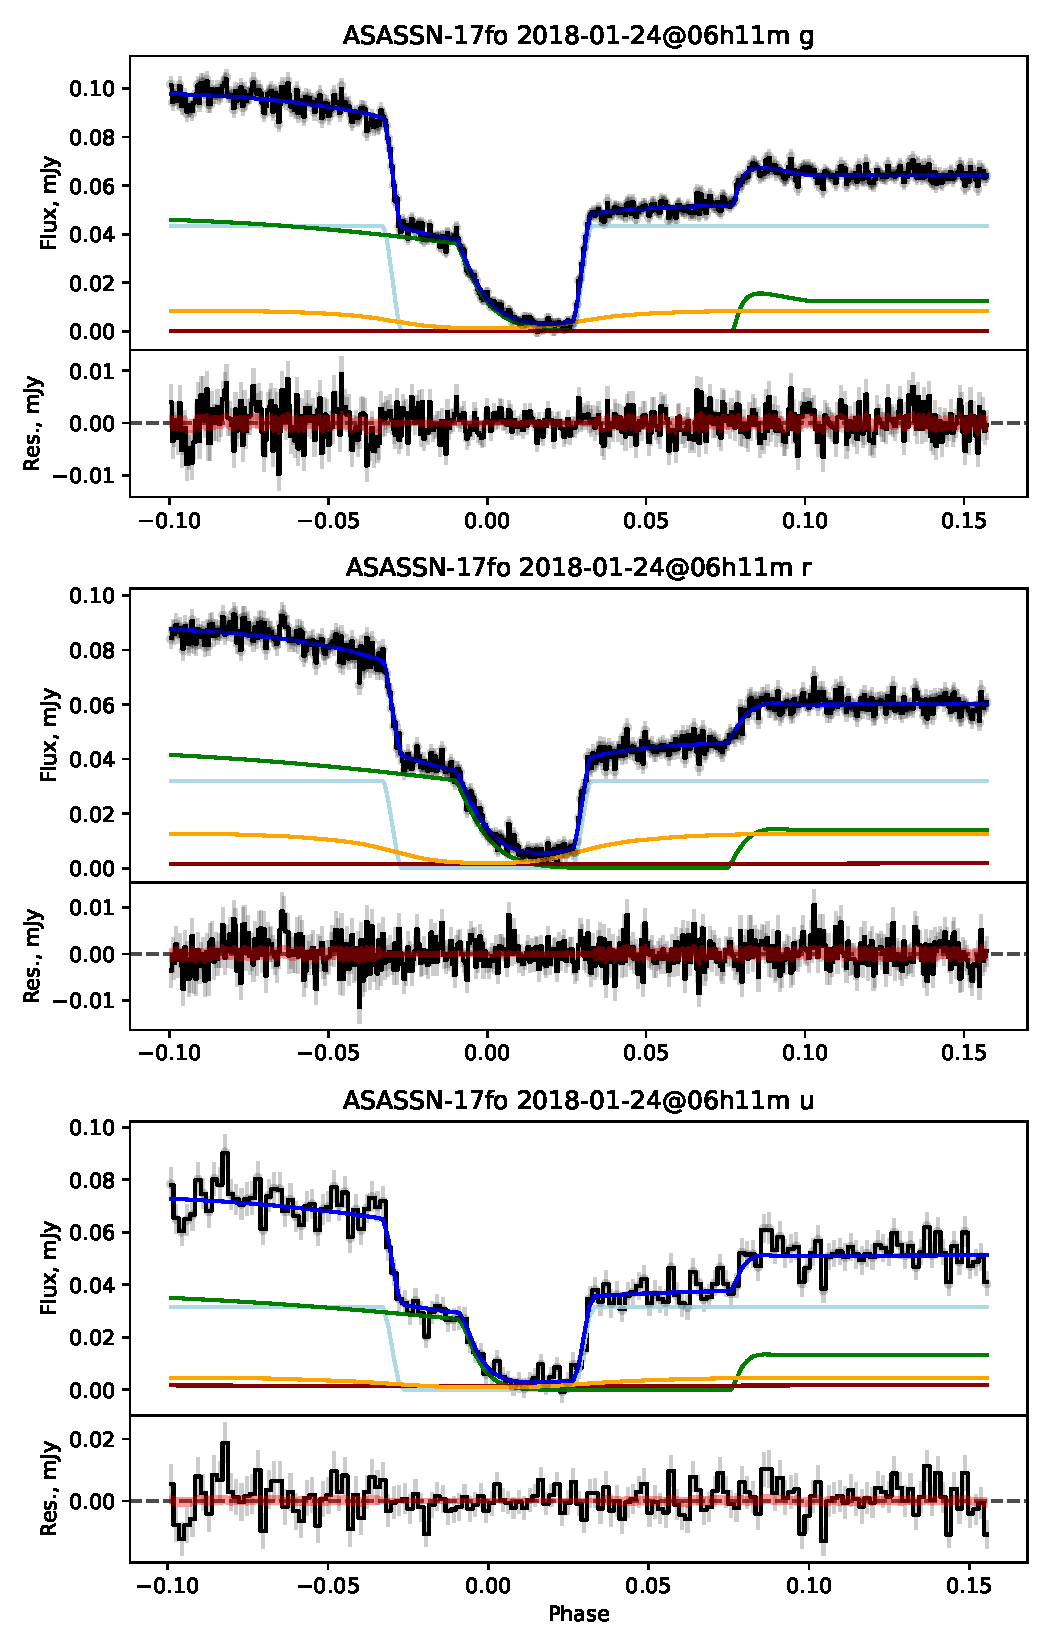
\includegraphics[width=\textwidth]{figures/results/ASASSN-17fo/ASASSN-17fo_1.pdf}
    \caption{ASASSN-17fo lightcurve models. Symbols are the same as Figure~\ref{fig:ASASSN-17jf all lightcurves}}
    \label{fig:ASASSN-17fo all lightcurves}
\end{figure}
\begin{figure}
    \centering
    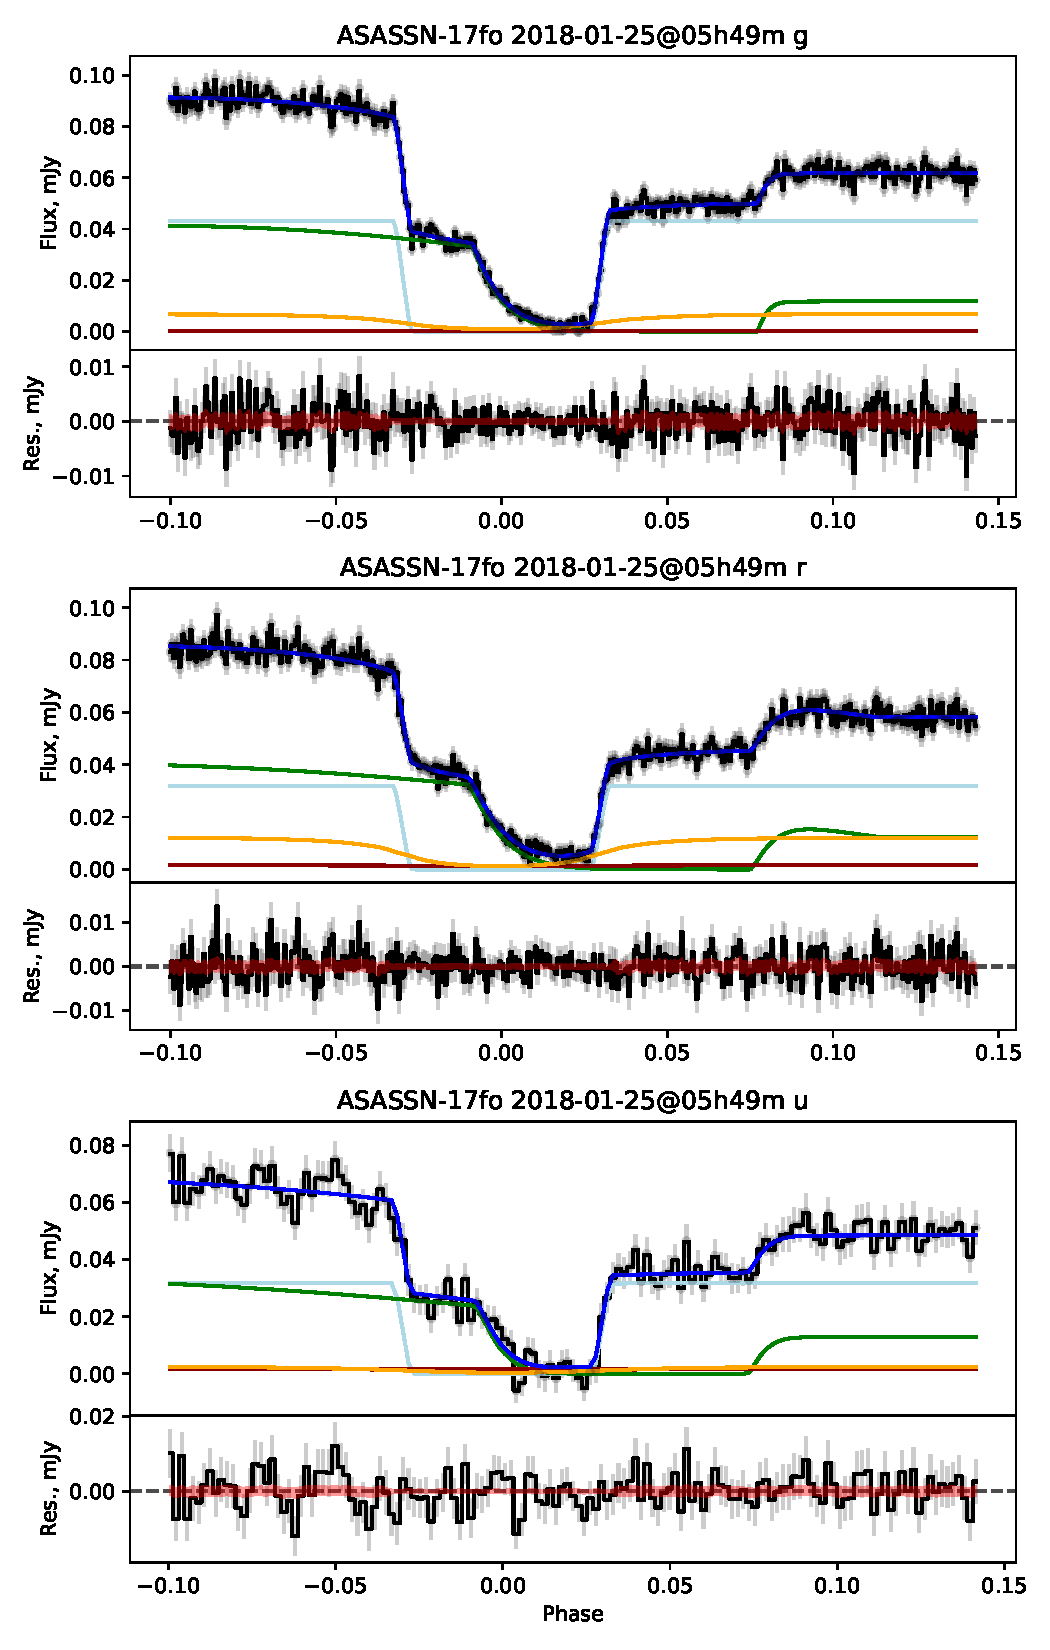
\includegraphics[width=\textwidth]{figures/results/ASASSN-17fo/ASASSN-17fo_2.pdf}
    \caption{ASASSN-17fo lightcurve models (cont.)}
    \label{fig:ASASSN-17fo all lightcurves cont 1}
\end{figure}
\begin{figure}
    \centering
    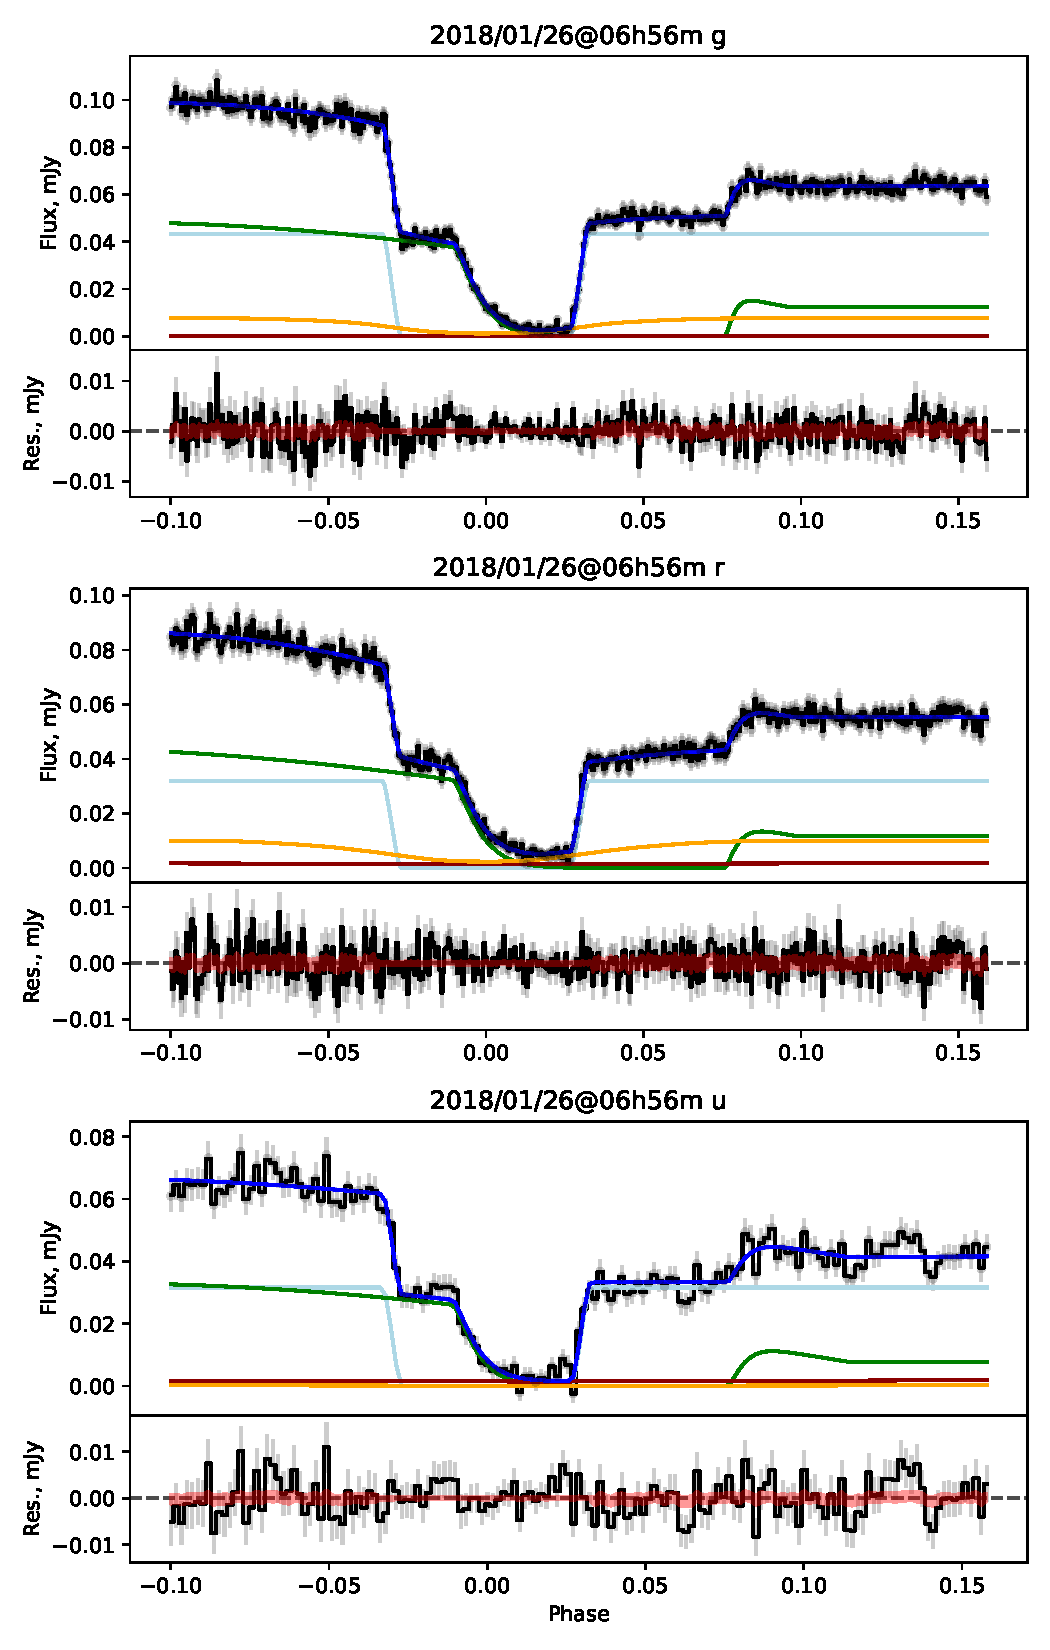
\includegraphics[width=\textwidth]{figures/results/ASASSN-17fo/ASASSN-17fo_3.pdf}
    \caption{ASASSN-17fo lightcurve models (cont.)}
    \label{fig:ASASSN-17fo all lightcurves cont 2}
\end{figure}



\begin{figure}
    \centering
    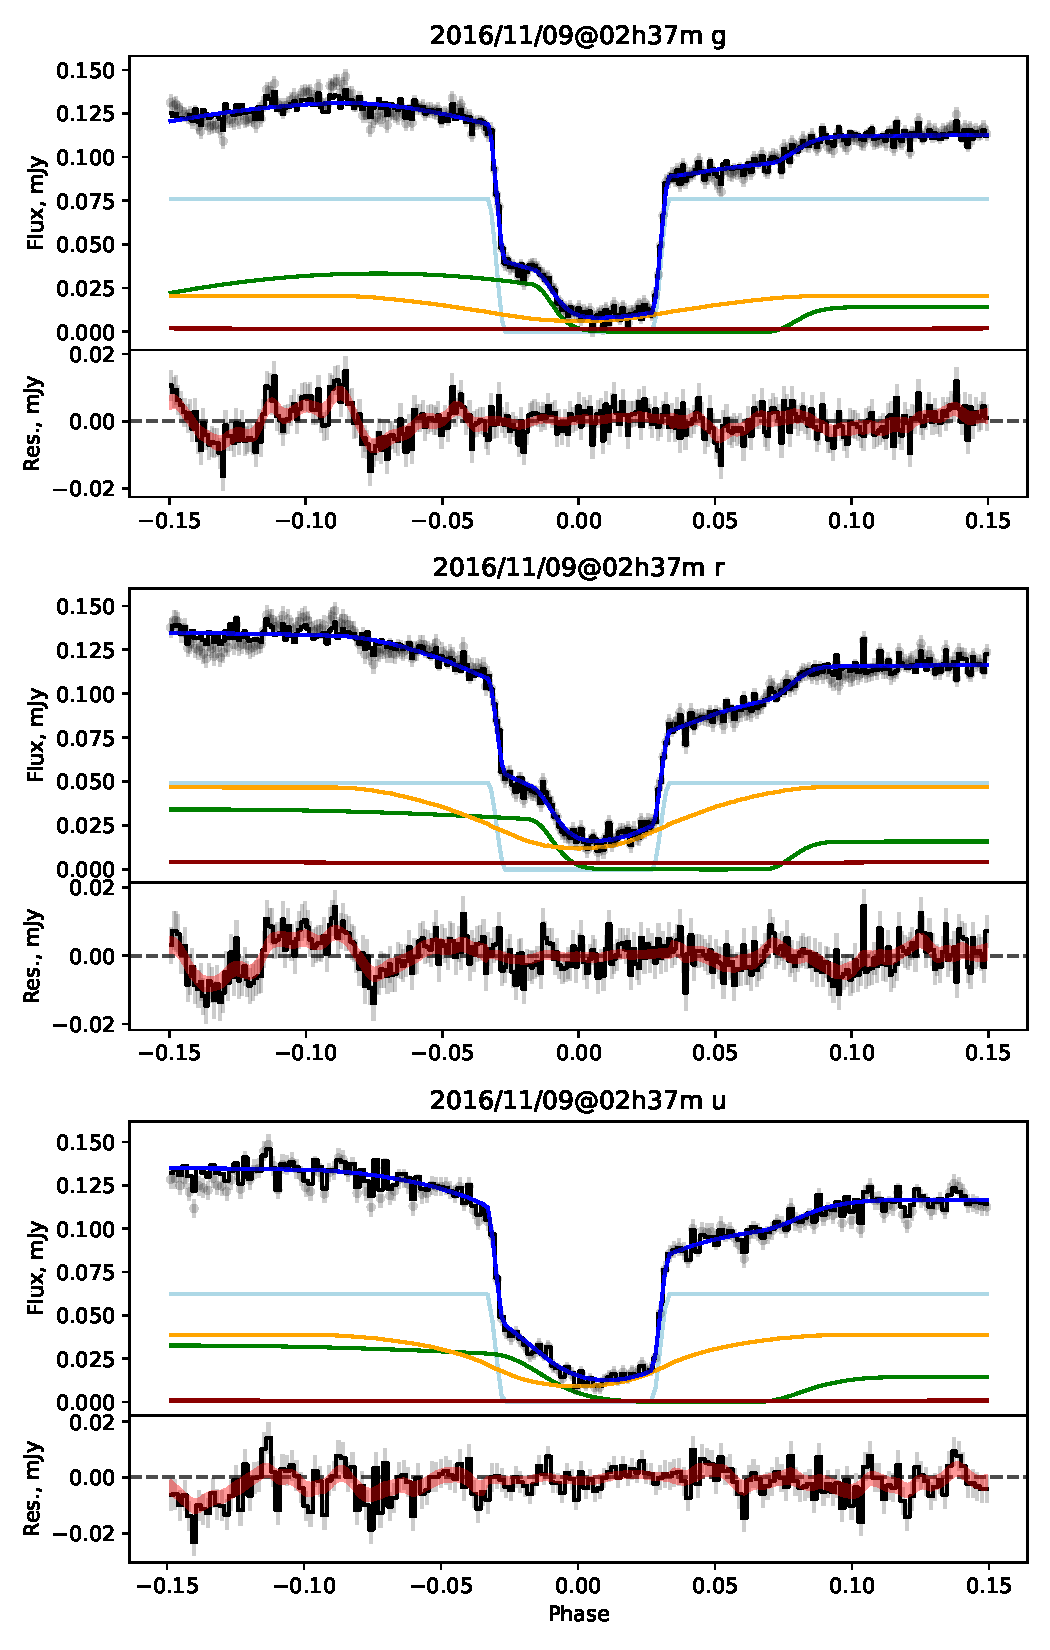
\includegraphics[width=\textwidth]{figures/results/AYFor/AYFor_1.pdf}
    \caption{AY For lightcurve models. Symbols are the same as Figure~\ref{fig:ASASSN-17jf all lightcurves}}
    \label{fig:AYFor all lightcurves}
\end{figure}
\begin{figure}
    \centering
    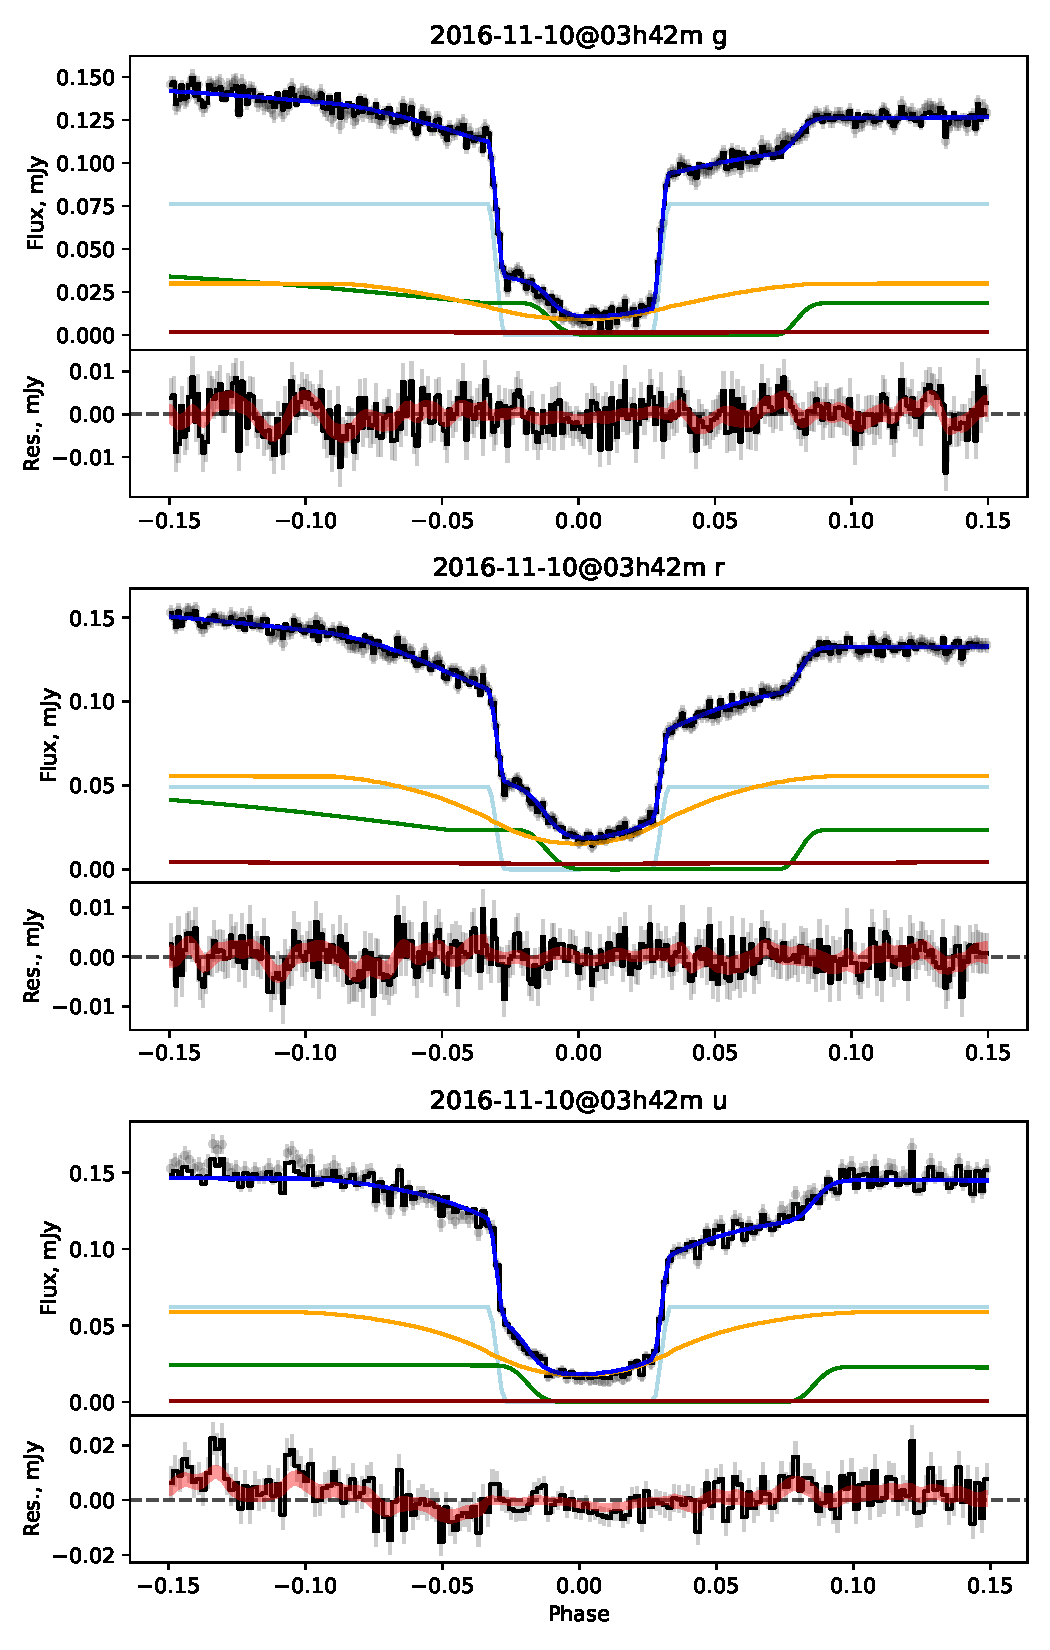
\includegraphics[width=\textwidth]{figures/results/AYFor/AYFor_2.pdf}
    \caption{AY For lightcurve models (cont.)}
    \label{fig:AYFor all lightcurves cont 1}
\end{figure}
\begin{figure}
    \centering
    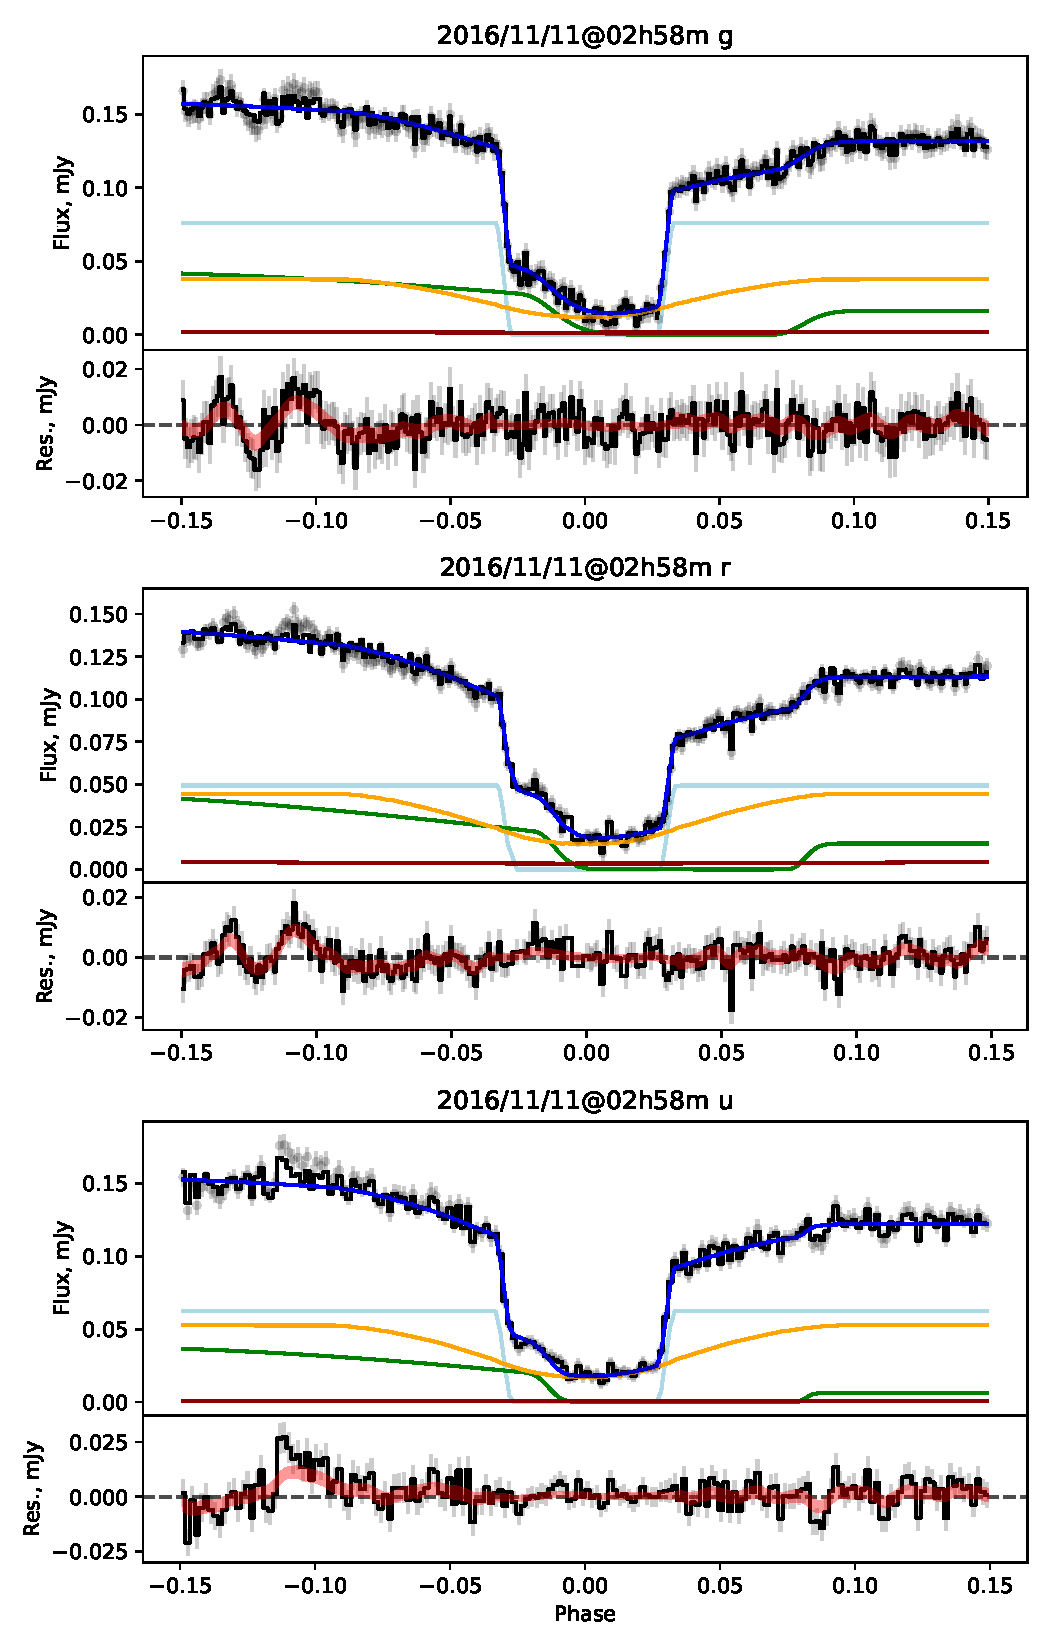
\includegraphics[width=\textwidth]{figures/results/AYFor/AYFor_3.pdf}
    \caption{AY For lightcurve models (cont.)}
    \label{fig:AYFor all lightcurves cont 2}
\end{figure}



\begin{figure}
    \centering
    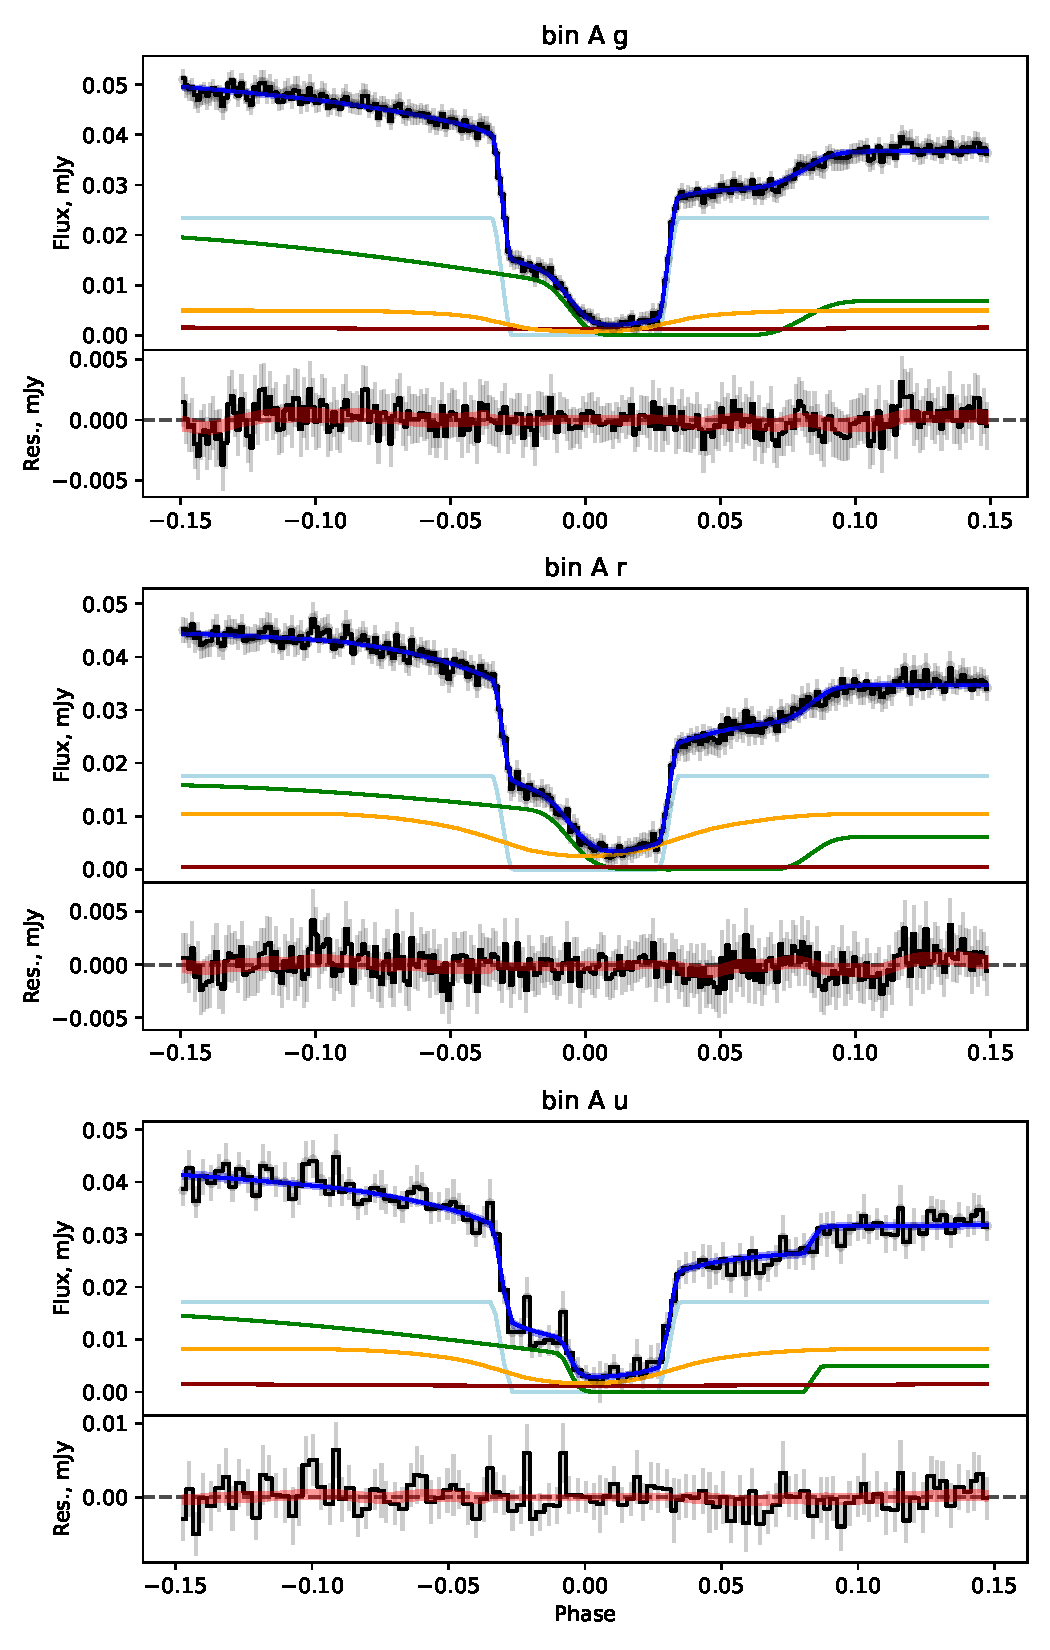
\includegraphics[width=\textwidth]{figures/results/CSS090102/CSS090102_1.pdf}
    \caption{CSS090102 lightcurve models. Symbols are the same as Figure~\ref{fig:ASASSN-17jf all lightcurves}}
    \label{fig:CSS090102 all lightcurves}
\end{figure}



\begin{figure}
    \centering
    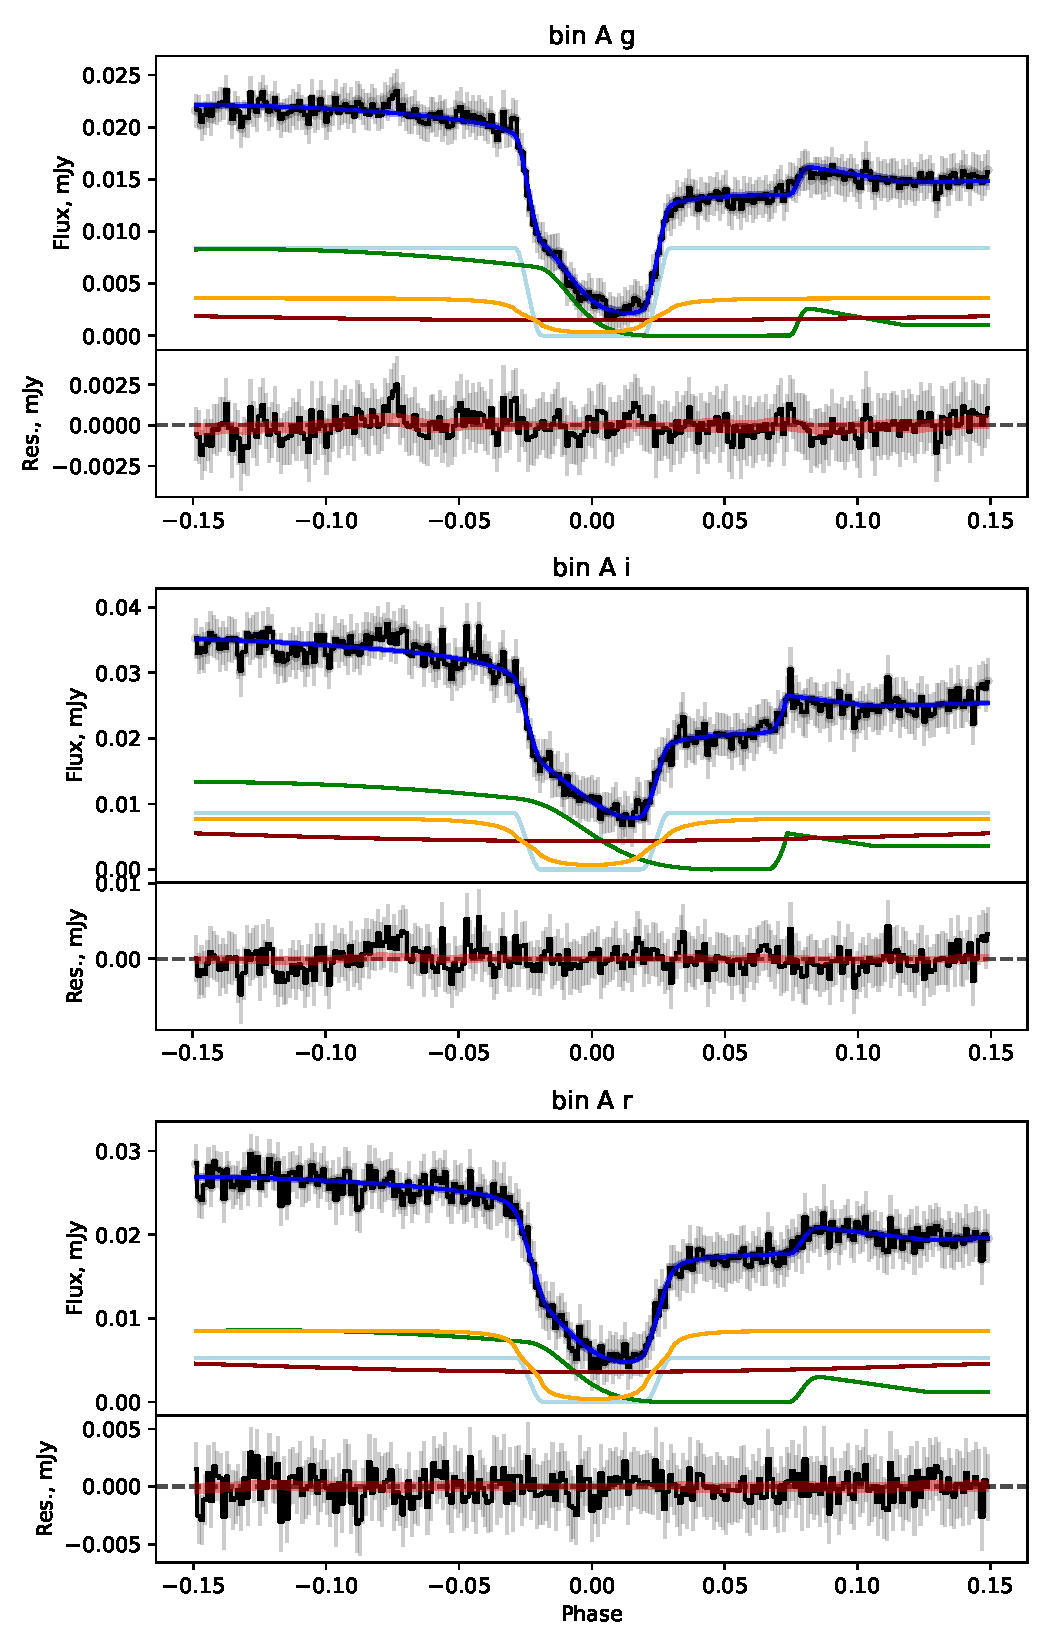
\includegraphics[width=\textwidth]{figures/results/CSS090419/CSS090419_1.pdf}
    \caption{CSS090419 lightcurve models. Symbols are the same as Figure~\ref{fig:ASASSN-17jf all lightcurves}}
    \label{fig:CSS090419 all lightcurves}
\end{figure}
\begin{figure}
    \centering
    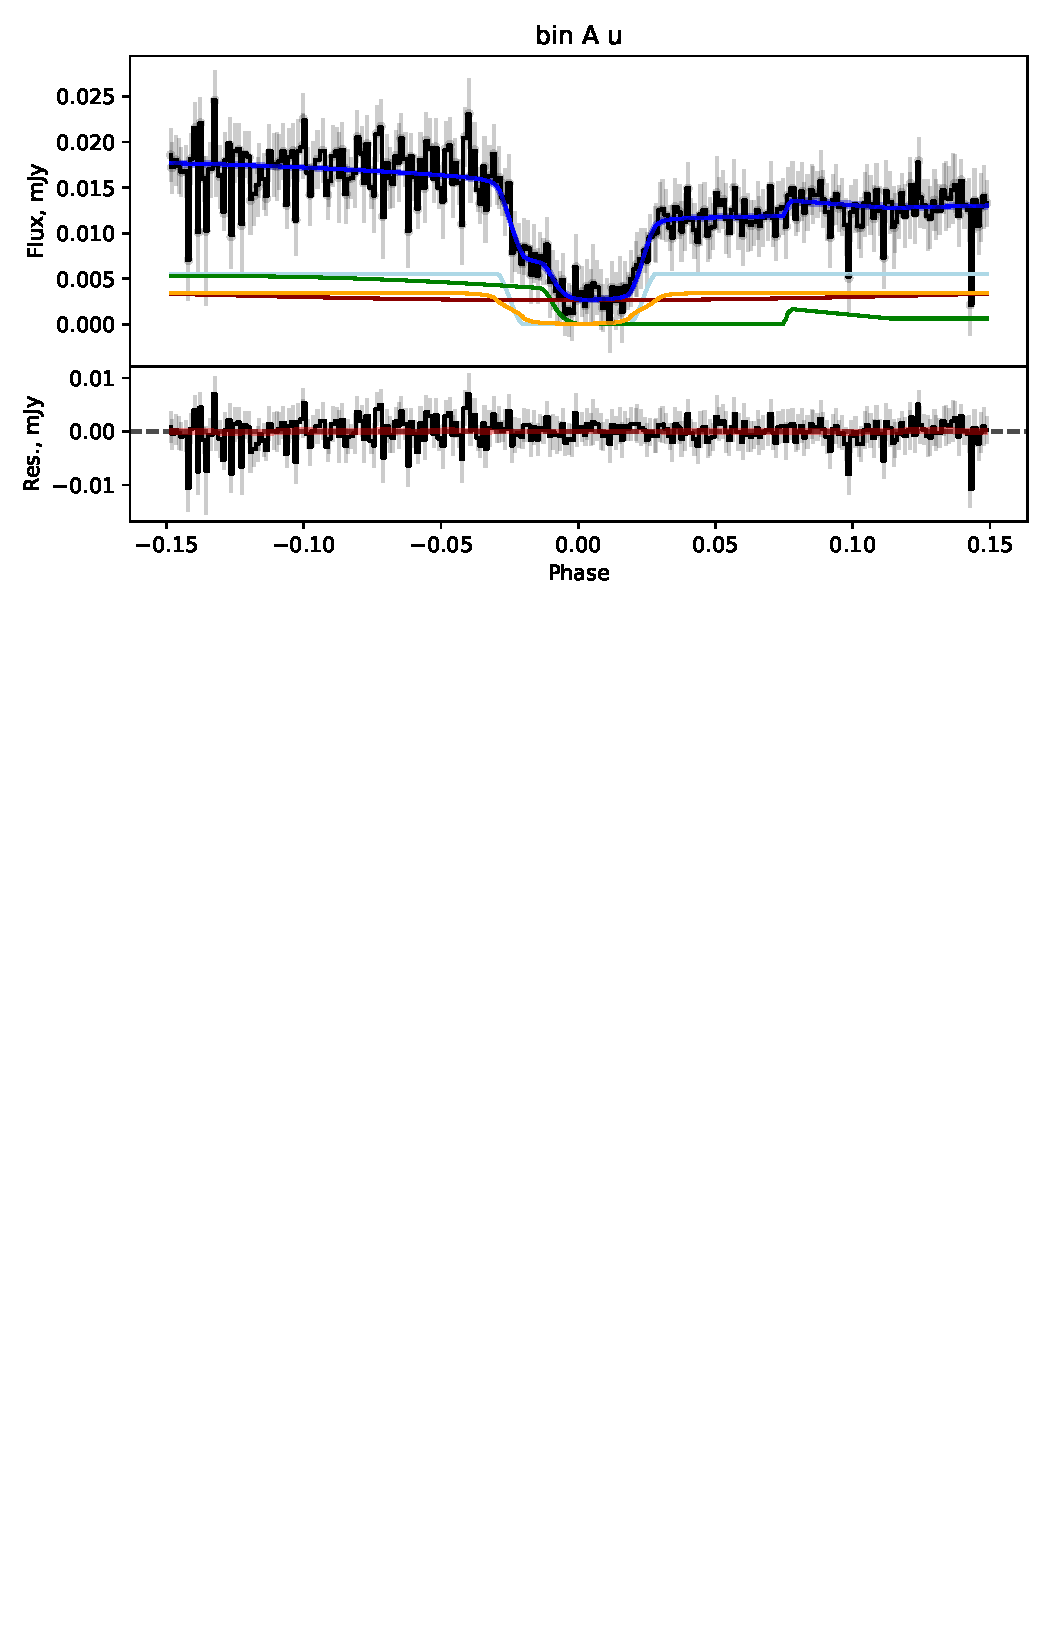
\includegraphics[width=\textwidth]{figures/results/CSS090419/CSS090419_2.pdf}
    \caption{CSS090419 lightcurve models (cont.)}
    \label{fig:CSS090419 all lightcurves cont 1}
\end{figure}



\begin{figure}
    \centering
    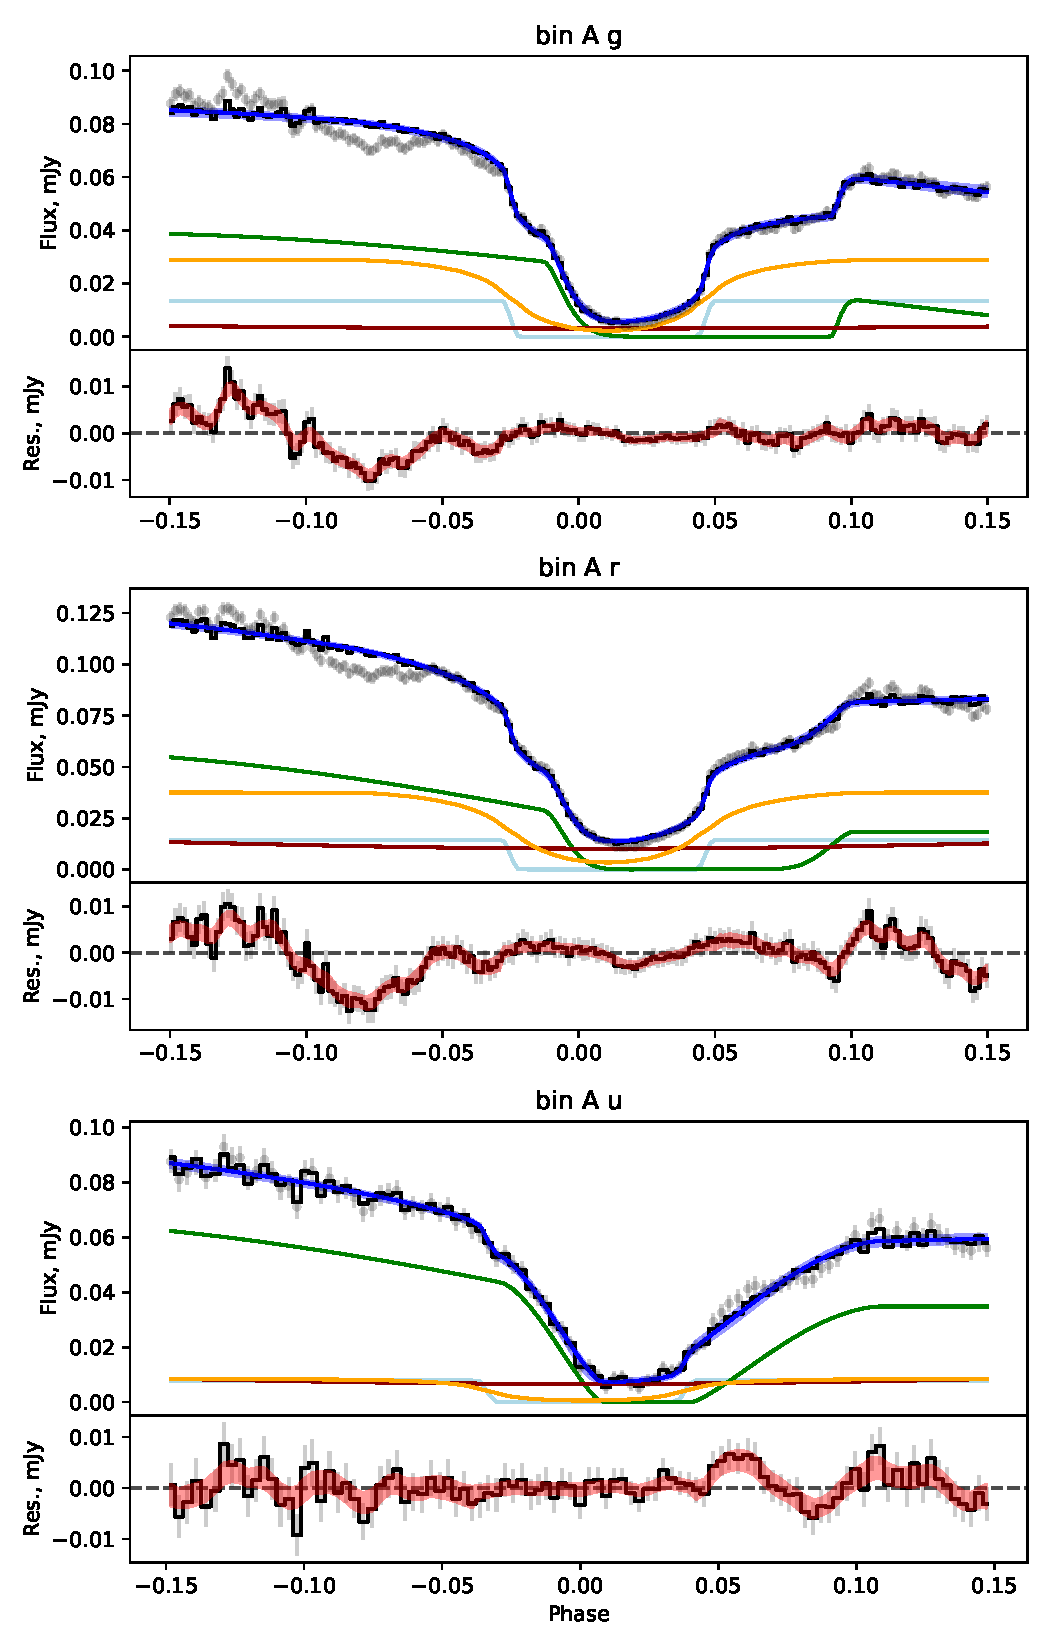
\includegraphics[width=\textwidth]{figures/results/CSS090622/CSS090622_1.pdf}
    \caption{CSS090622 lightcurve models. Symbols are the same as Figure~\ref{fig:ASASSN-17jf all lightcurves}}
    \label{fig:CSS090622 all lightcurves}
\end{figure}
\begin{figure}
    \centering
    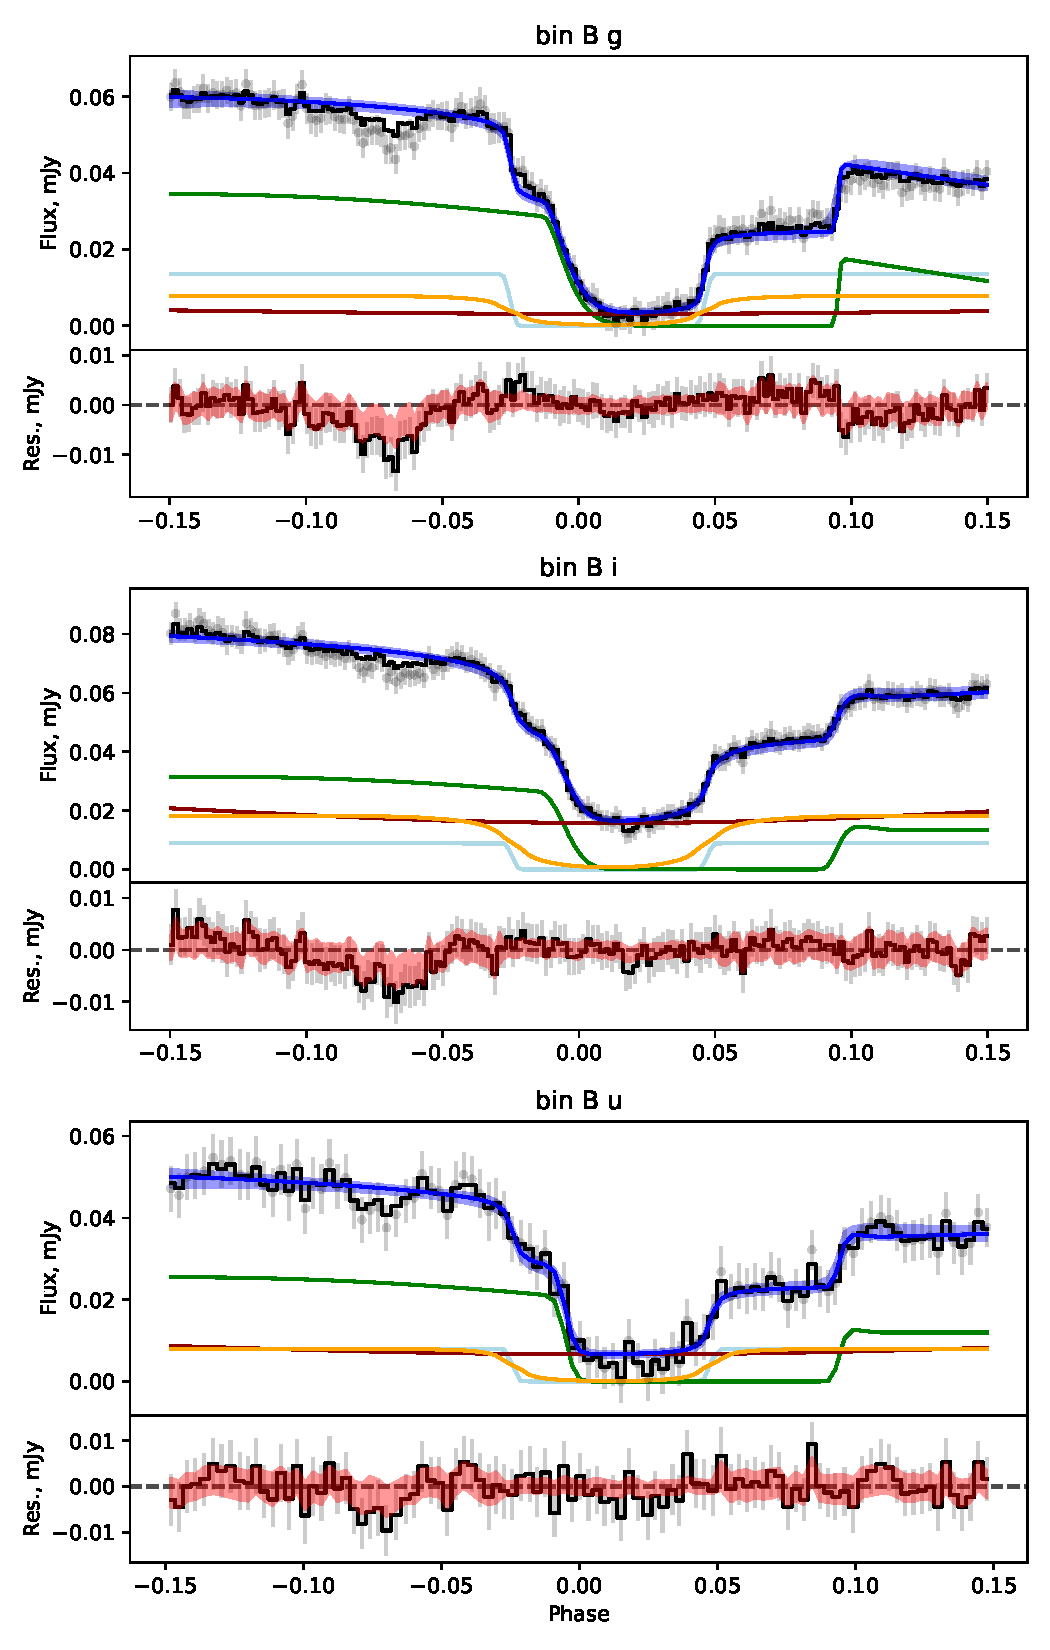
\includegraphics[width=\textwidth]{figures/results/CSS090622/CSS090622_2.pdf}
    \caption{CSS090622 lightcurve models (cont.)}
    \label{fig:CSS090622 all lightcurves cont 1}
\end{figure}



\begin{figure}
    \centering
    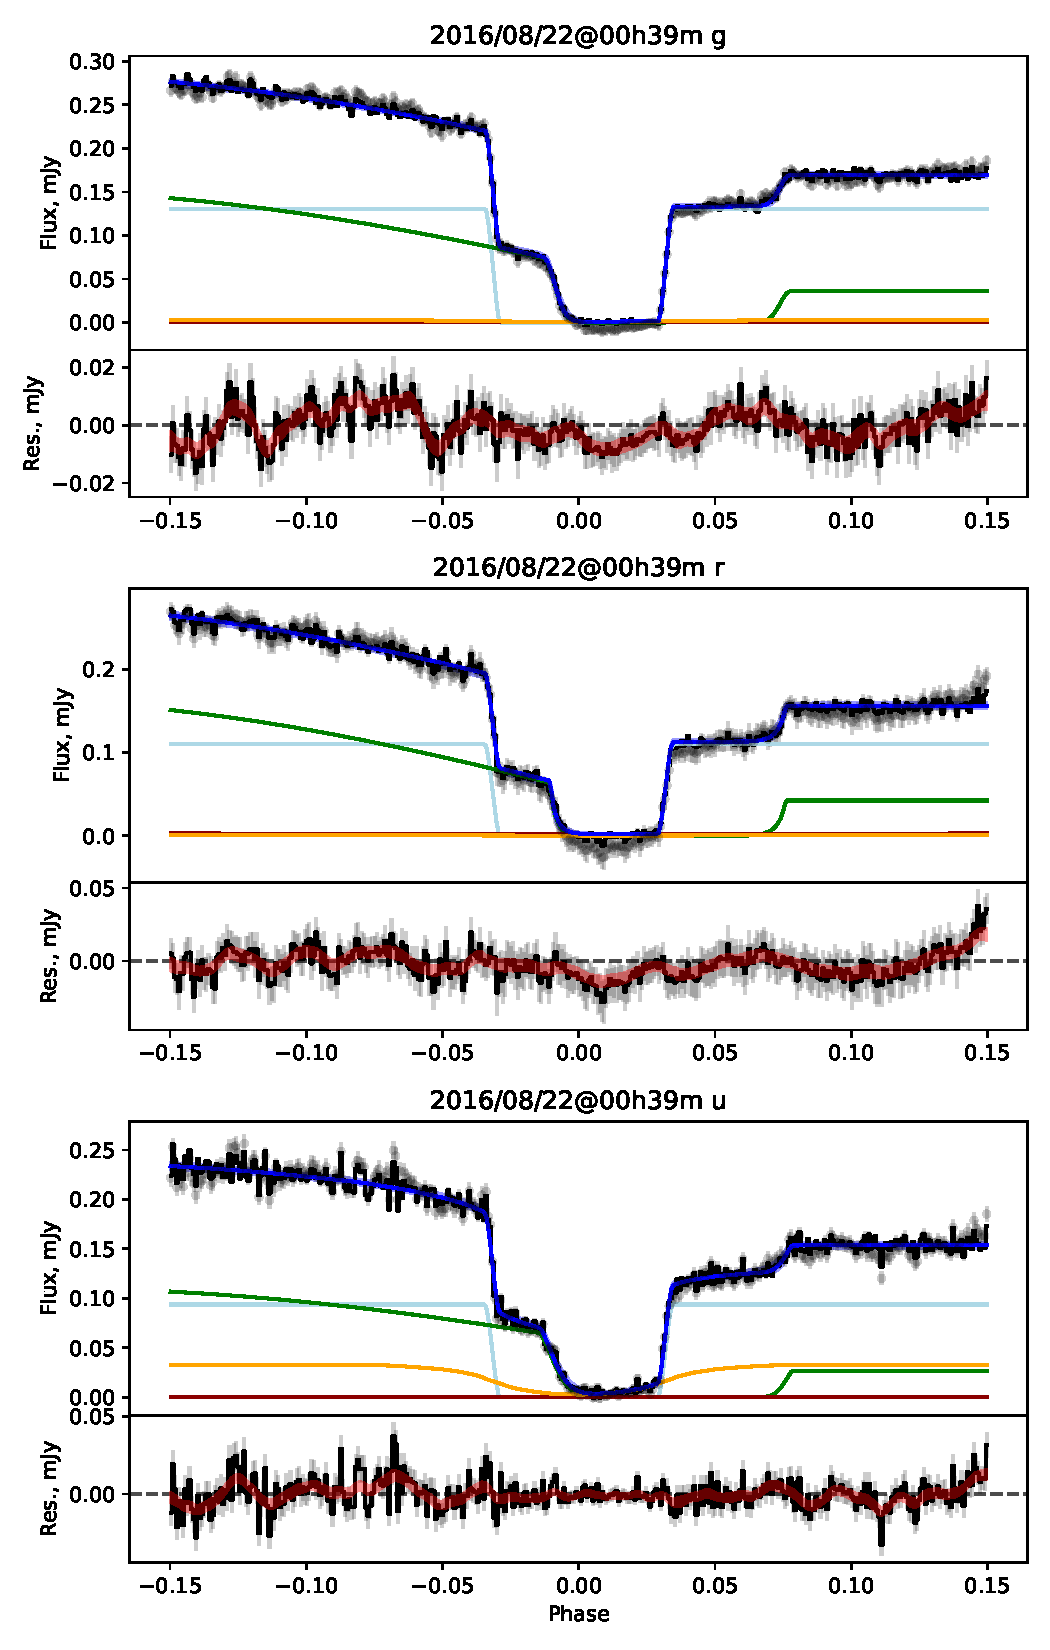
\includegraphics[width=\textwidth]{figures/results/OGLE82/OGLE82_1.pdf}
    \caption{OGLE82 lightcurve models. Symbols are the same as Figure~\ref{fig:ASASSN-17jf all lightcurves}}
    \label{fig:OGLE82 all lightcurves}
\end{figure}
\begin{figure}
    \centering
    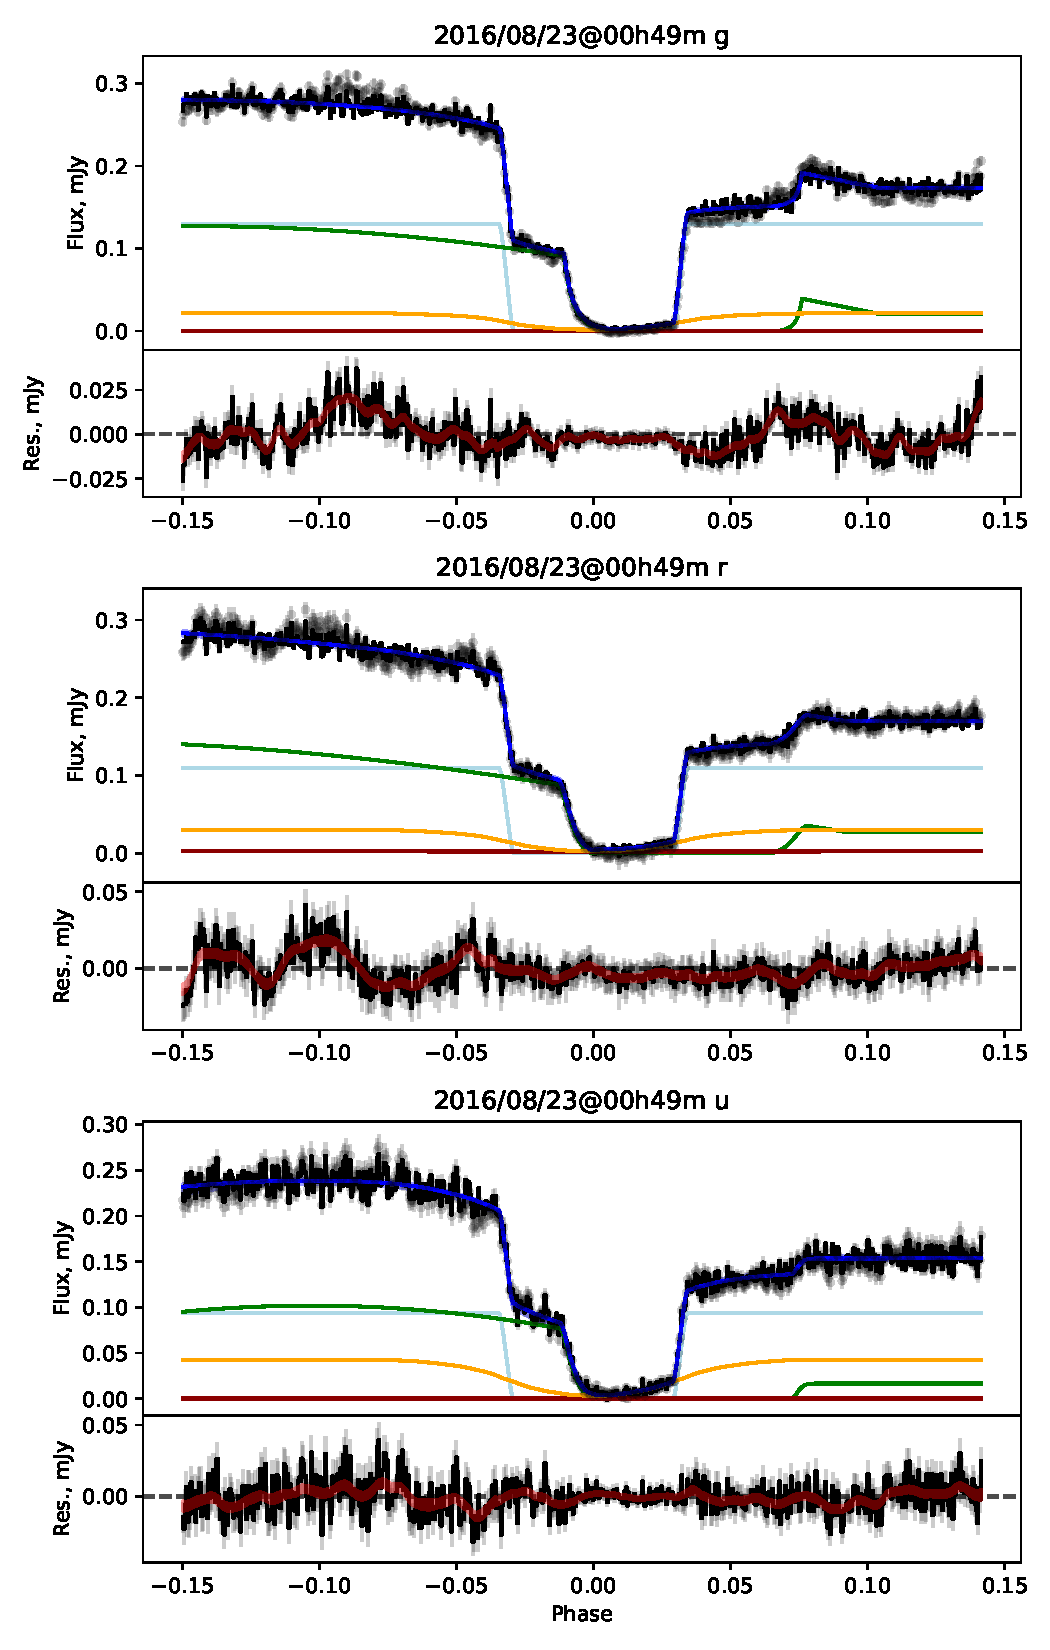
\includegraphics[width=\textwidth]{figures/results/OGLE82/OGLE82_2.pdf}
    \caption{OGLE82 lightcurve models (cont.)}
    \label{fig:OGLE82 all lightcurves cont 1}
\end{figure}



\begin{figure}
    \centering
    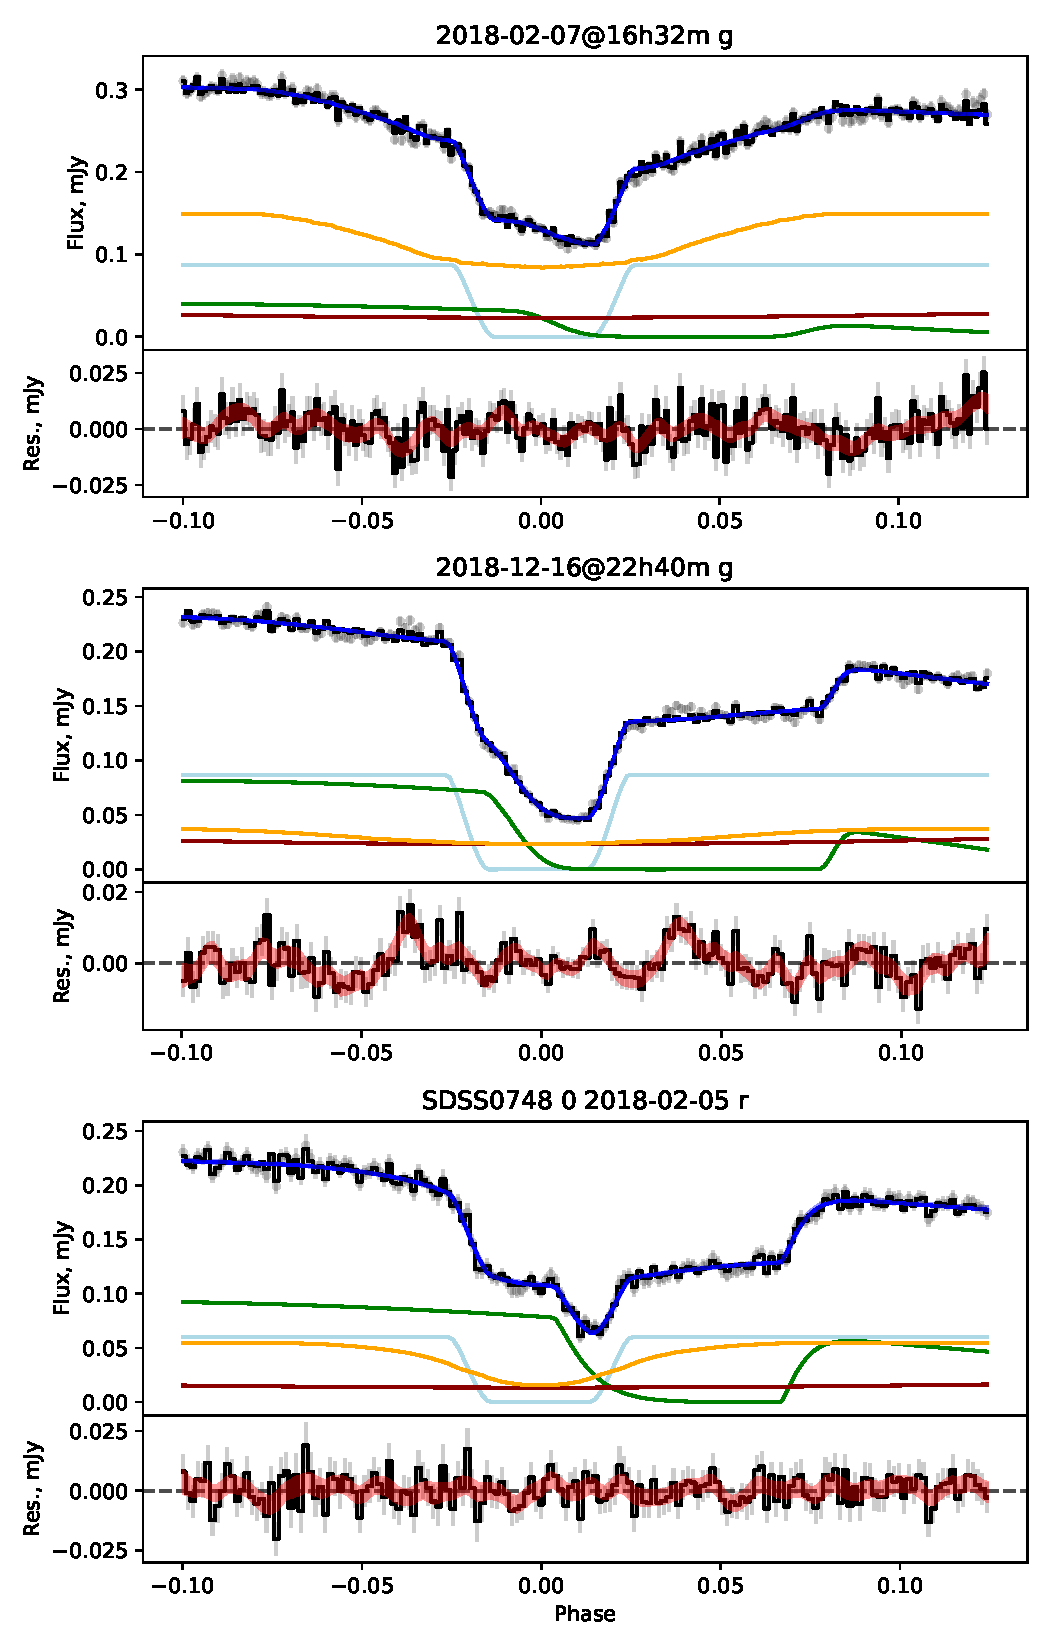
\includegraphics[width=\textwidth]{figures/results/SDSS0748/SDSS0748_1.pdf}
    \caption{SDSS J0748 lightcurve models. Symbols are the same as Figure~\ref{fig:ASASSN-17jf all lightcurves}}
    \label{fig:SDSS J0748 all lightcurves}
\end{figure}
\begin{figure}
    \centering
    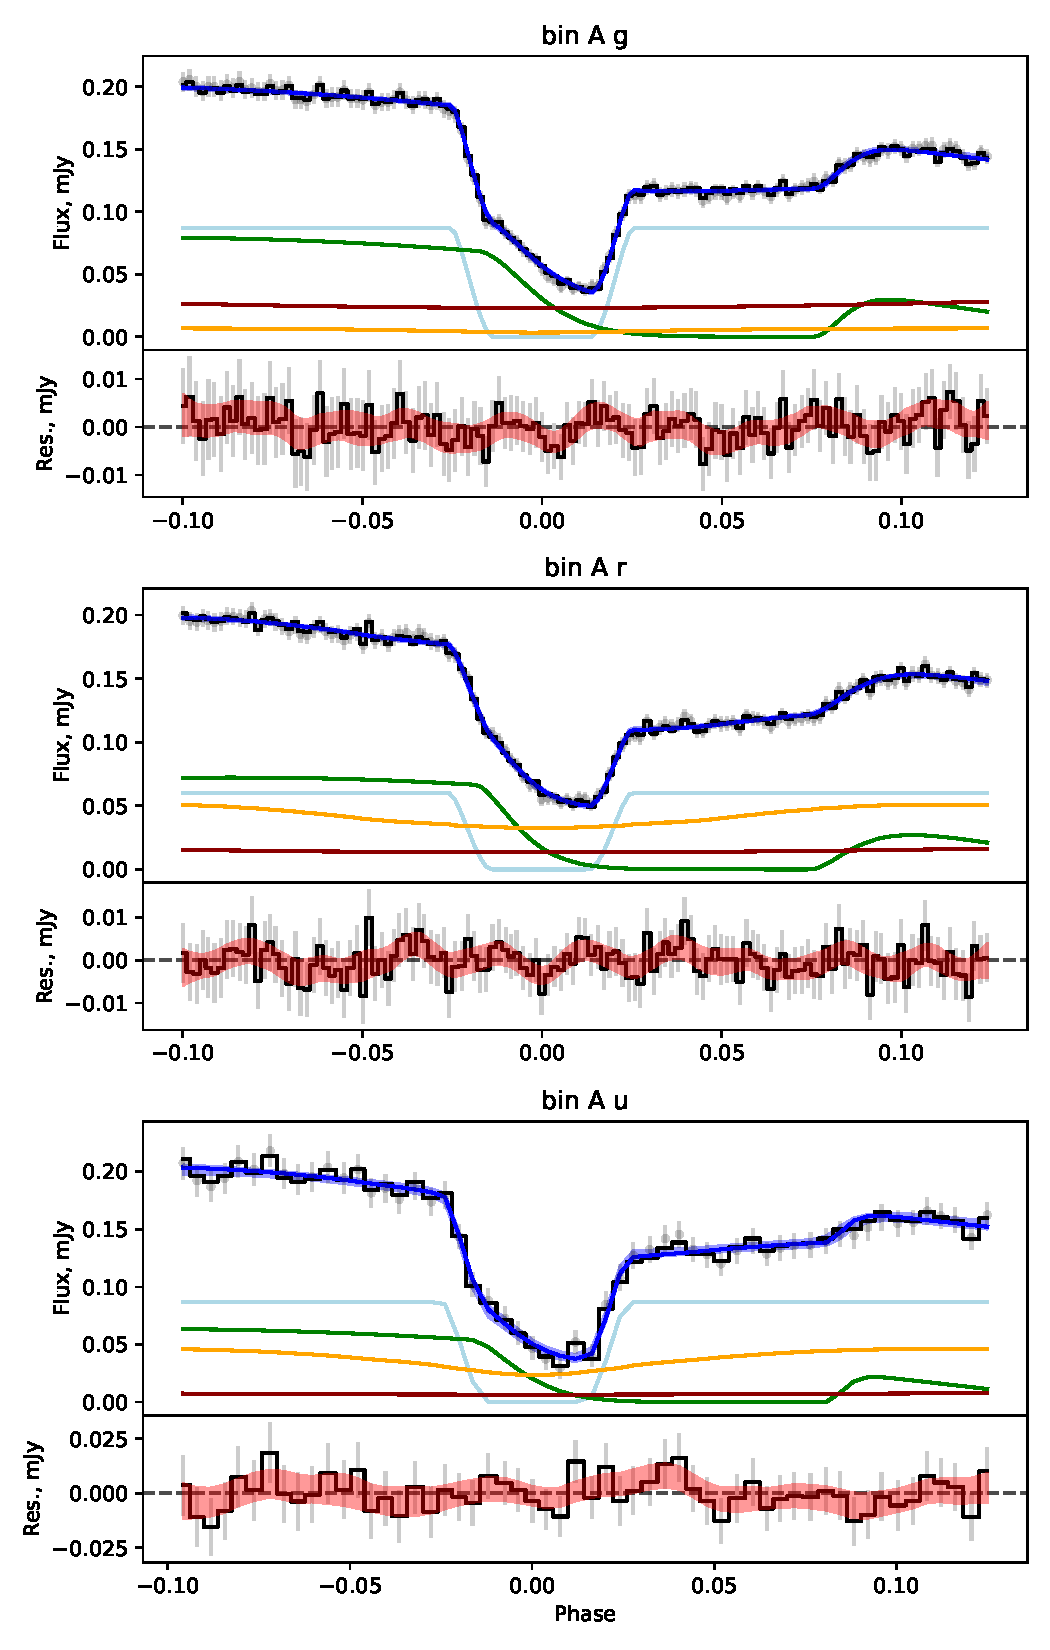
\includegraphics[width=\textwidth]{figures/results/SDSS0748/SDSS0748_2.pdf}
    \caption{SDSS J0748 lightcurve models (cont.)}
    \label{fig:SDSS J0748 all lightcurves cont 1}
\end{figure}
\begin{figure}
    \centering
    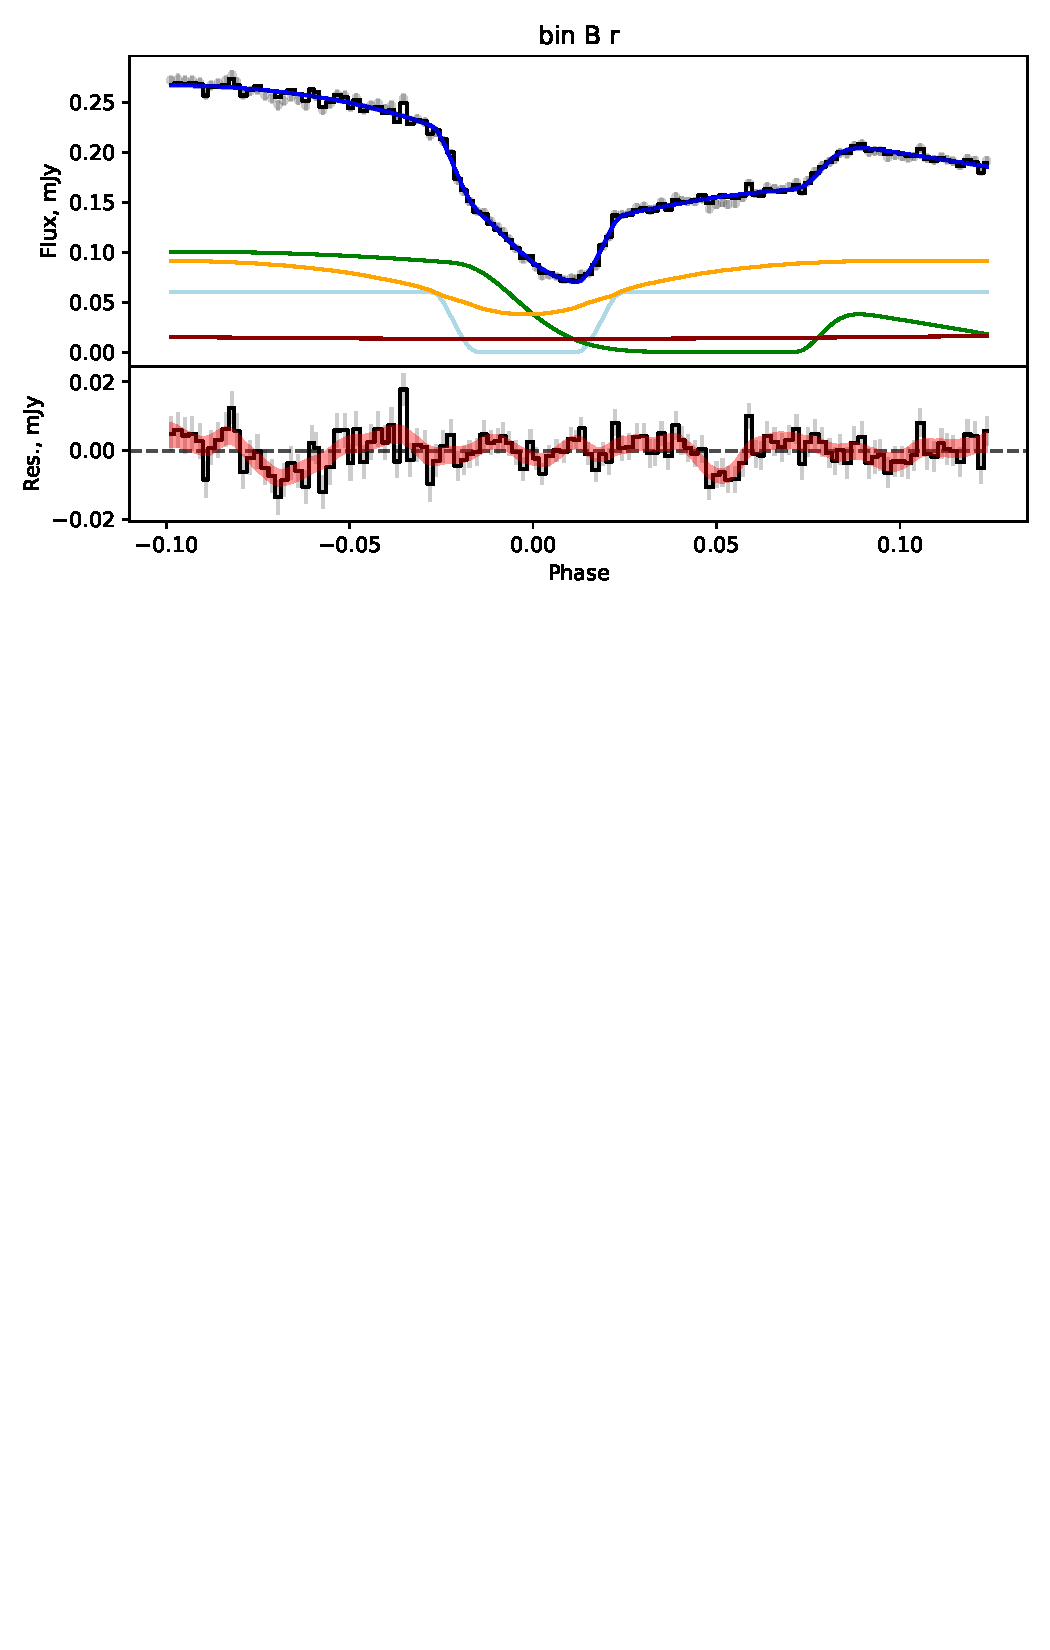
\includegraphics[width=\textwidth]{figures/results/SDSS0748/SDSS0748_3.pdf}
    \caption{SDSS J0748 lightcurve models (cont.)}
    \label{fig:SDSS J0748 all lightcurves cont 2}
\end{figure}



\begin{figure}
    \centering
    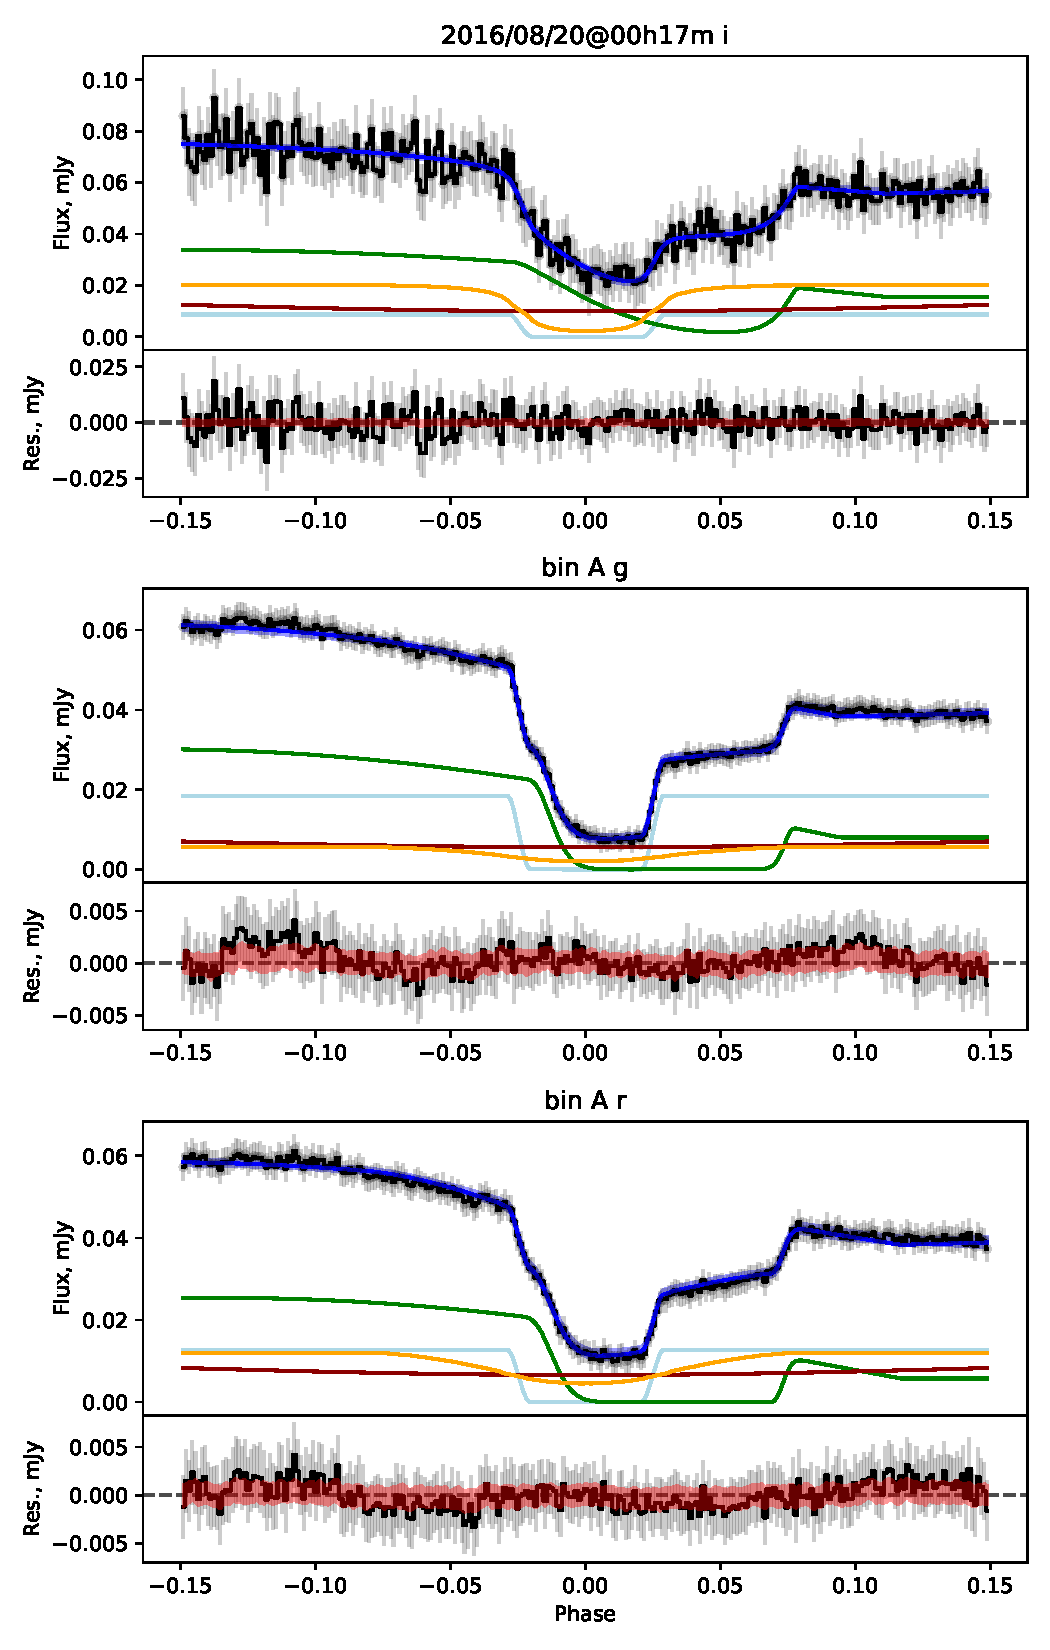
\includegraphics[width=\textwidth]{figures/results/ASASSN-15pb/ASASSN-15pb_1.pdf}
    \caption{ASASSN-15pb lightcurve models. Symbols are the same as Figure~\ref{fig:ASASSN-17jf all lightcurves}}
    \label{fig:ASASSN-15pb all lightcurves}
\end{figure}
\begin{figure}
    \centering
    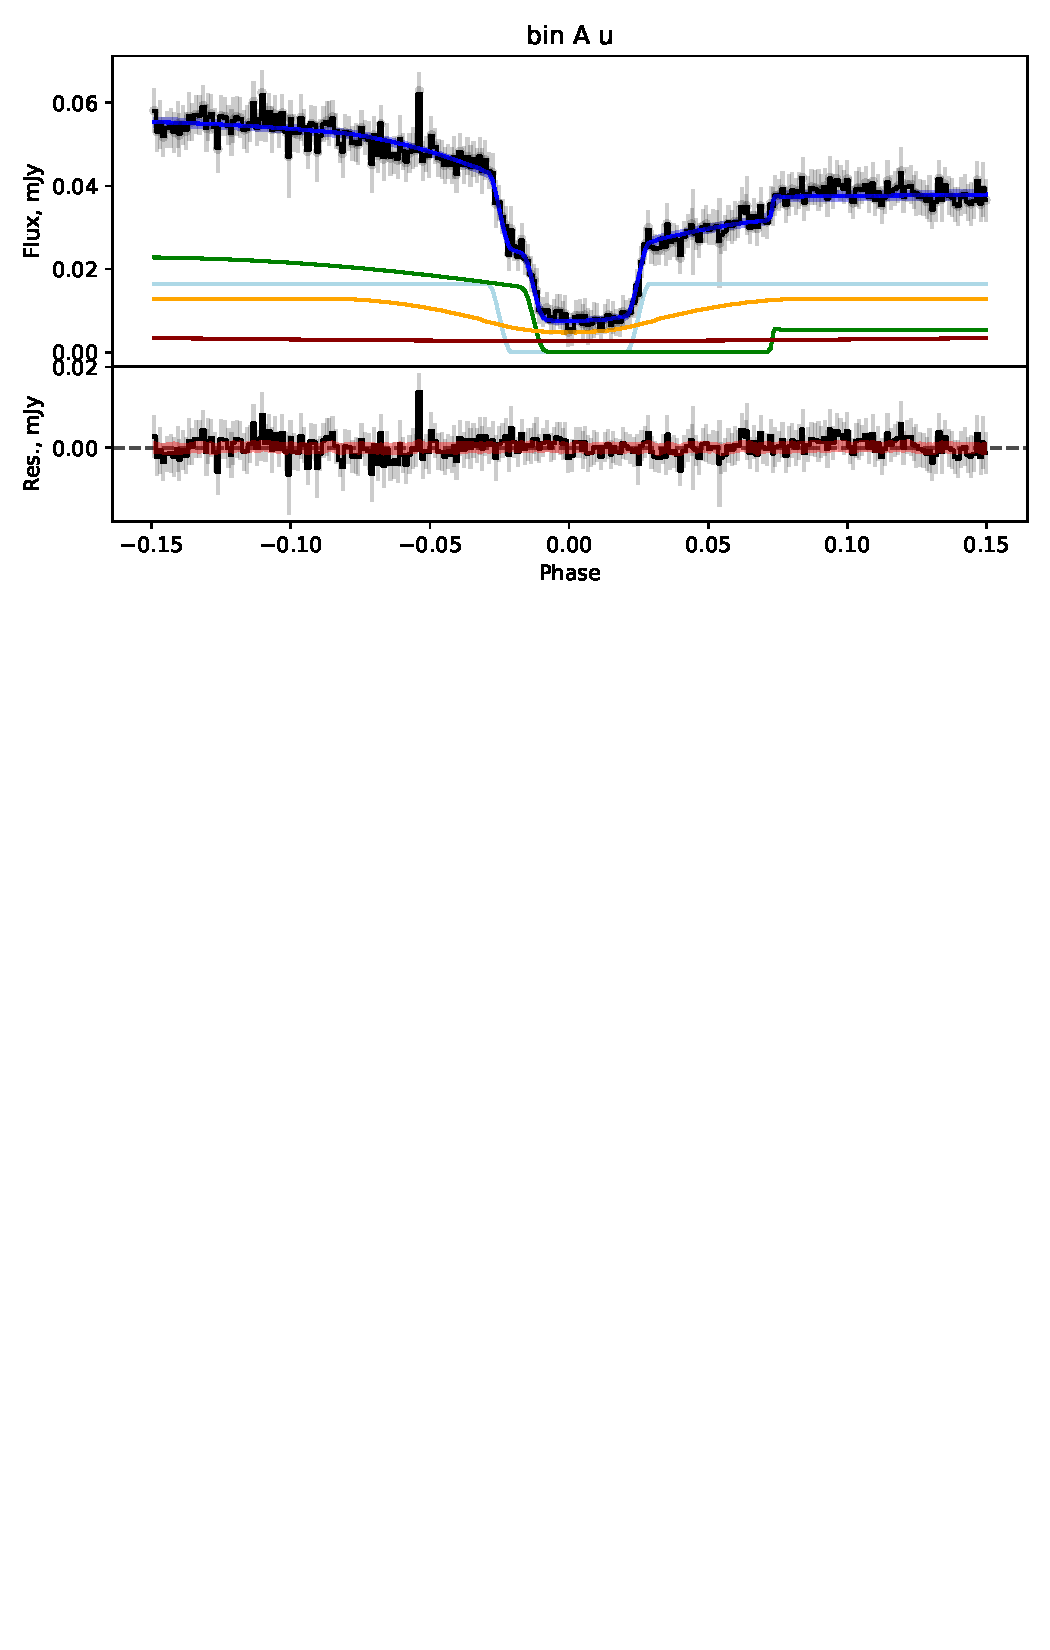
\includegraphics[width=\textwidth]{figures/results/ASASSN-15pb/ASASSN-15pb_2.pdf}
    \caption{ASASSN-15pb lightcurve models (cont.)}
    \label{fig:ASASSN-15pb all lightcurves cont 1}
\end{figure}



\begin{figure}
    \centering
    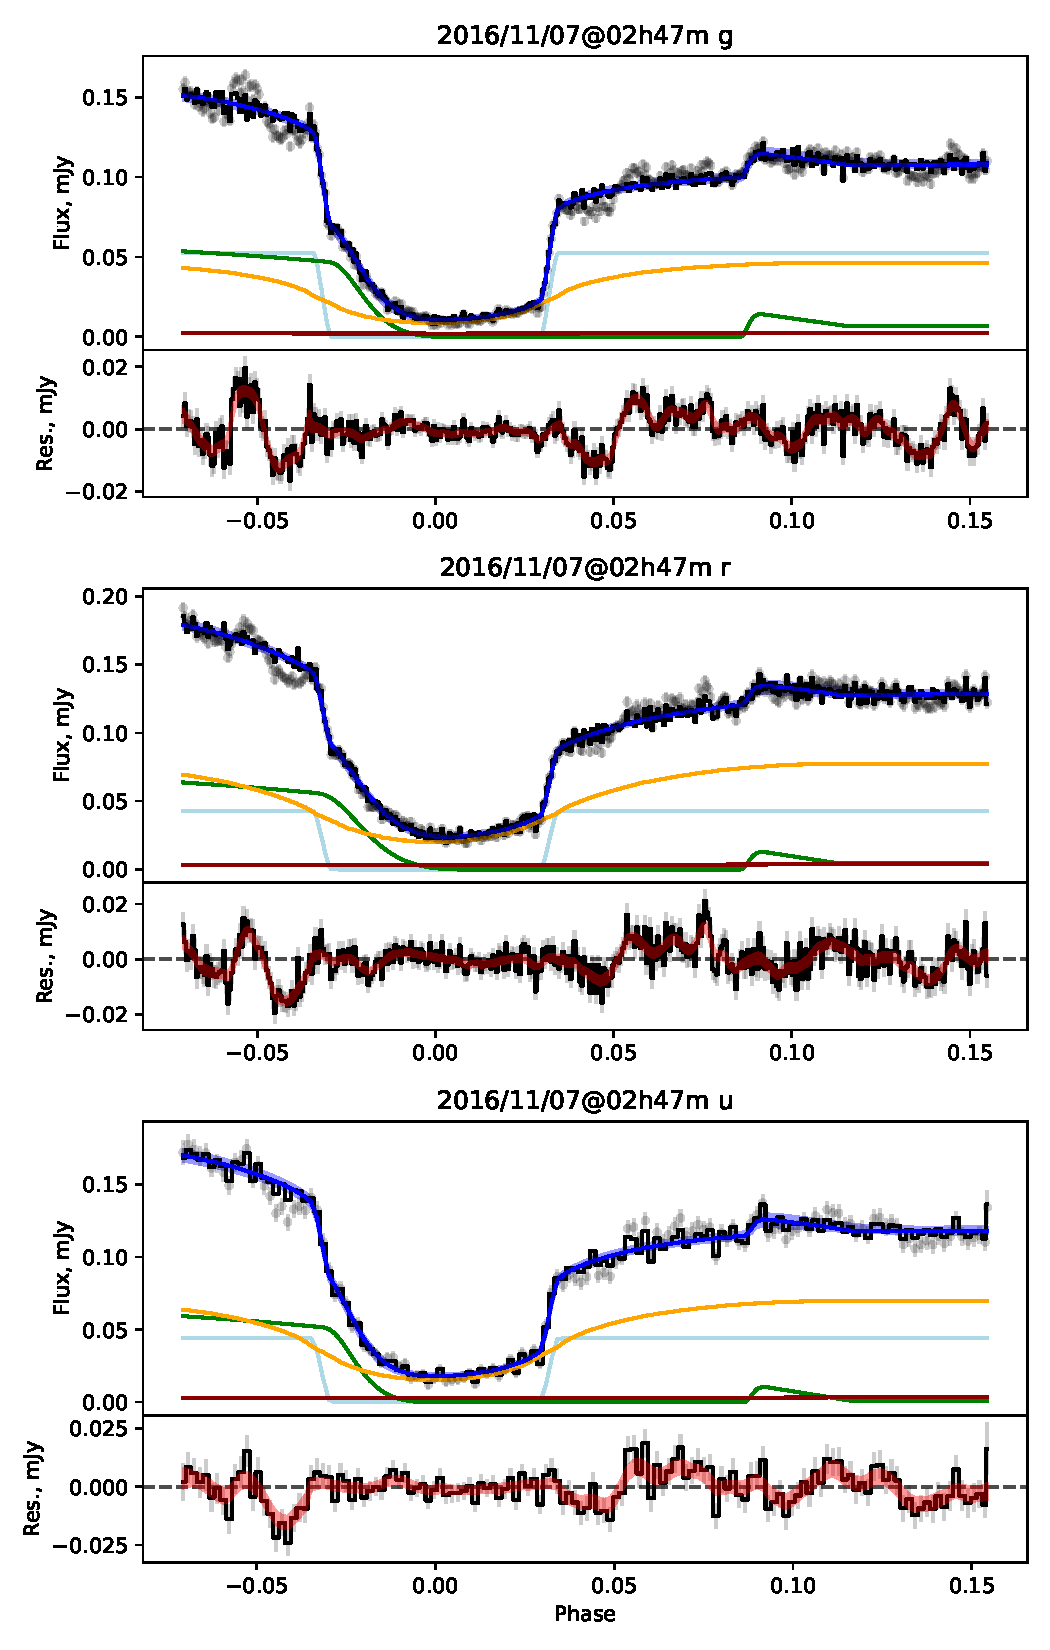
\includegraphics[width=\textwidth]{figures/results/MASOT0014/MASOT0014_1.pdf}
    \caption{MAS0014 lightcurve models. Symbols are the same as Figure~\ref{fig:ASASSN-17jf all lightcurves}}
    \label{fig:MAS0014 all lightcurves}
\end{figure}
\begin{figure}
    \centering
    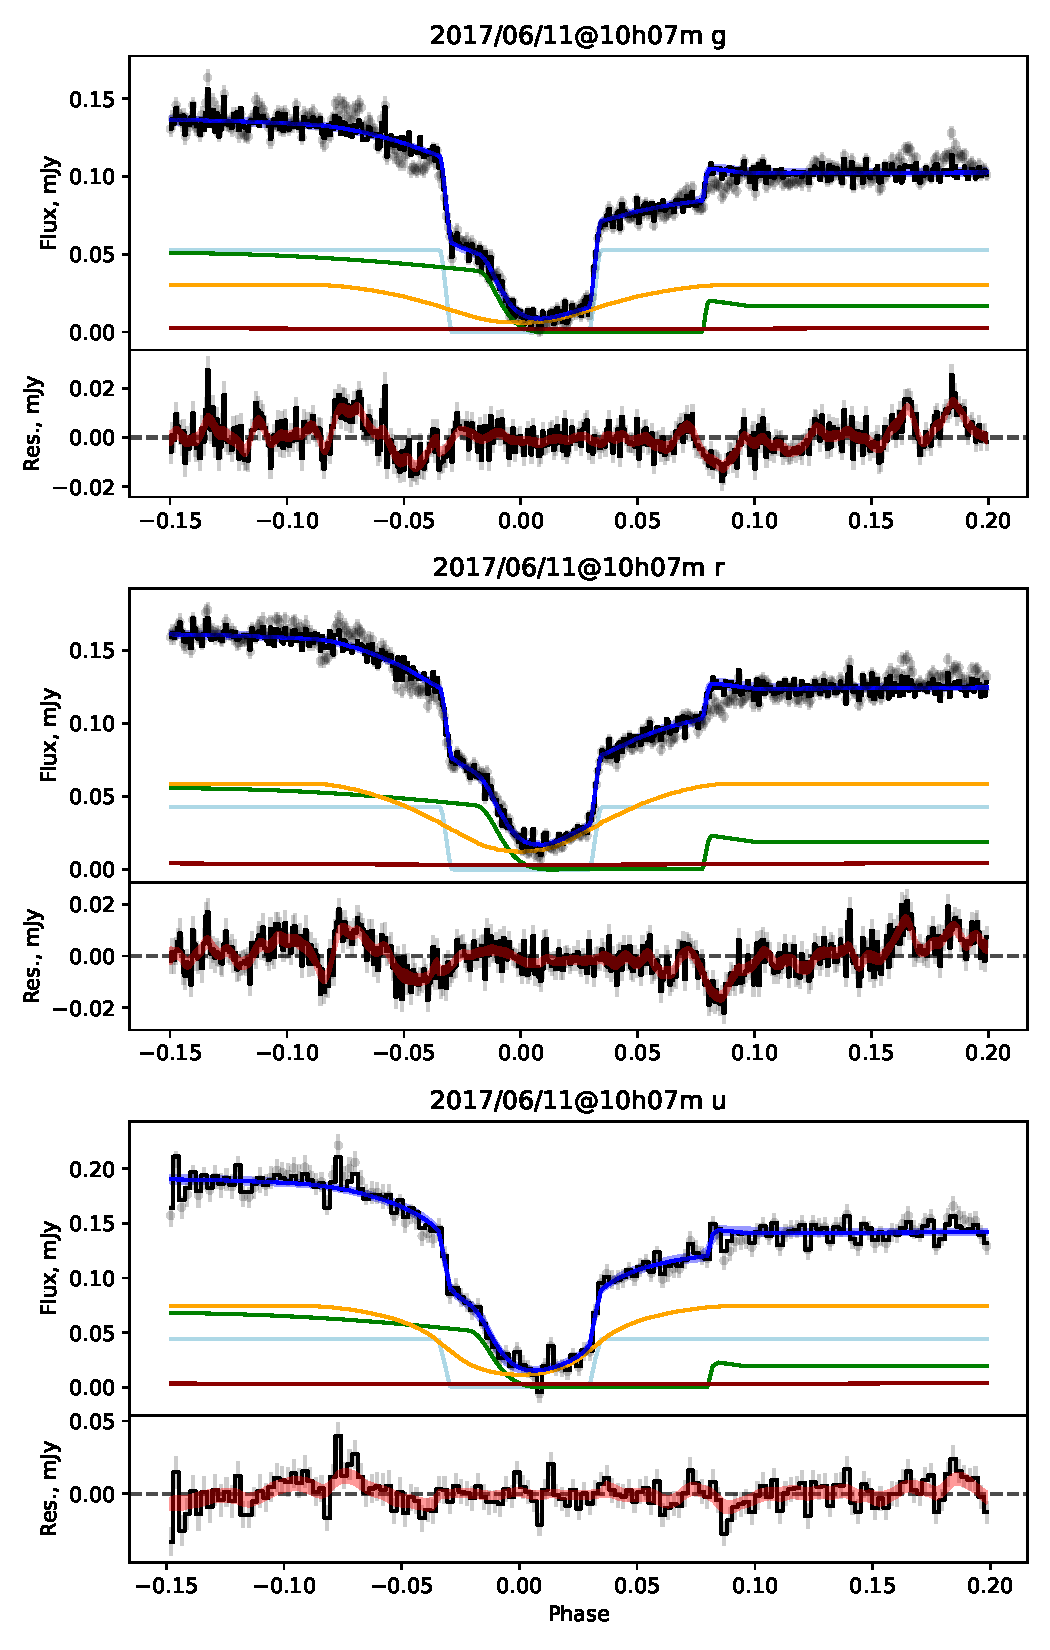
\includegraphics[width=\textwidth]{figures/results/MASOT0014/MASOT0014_2.pdf}
    \caption{MAS0014 lightcurve models (cont.)}
    \label{fig:MAS0014 all lightcurves cont 1}
\end{figure}
\begin{figure}
    \centering
    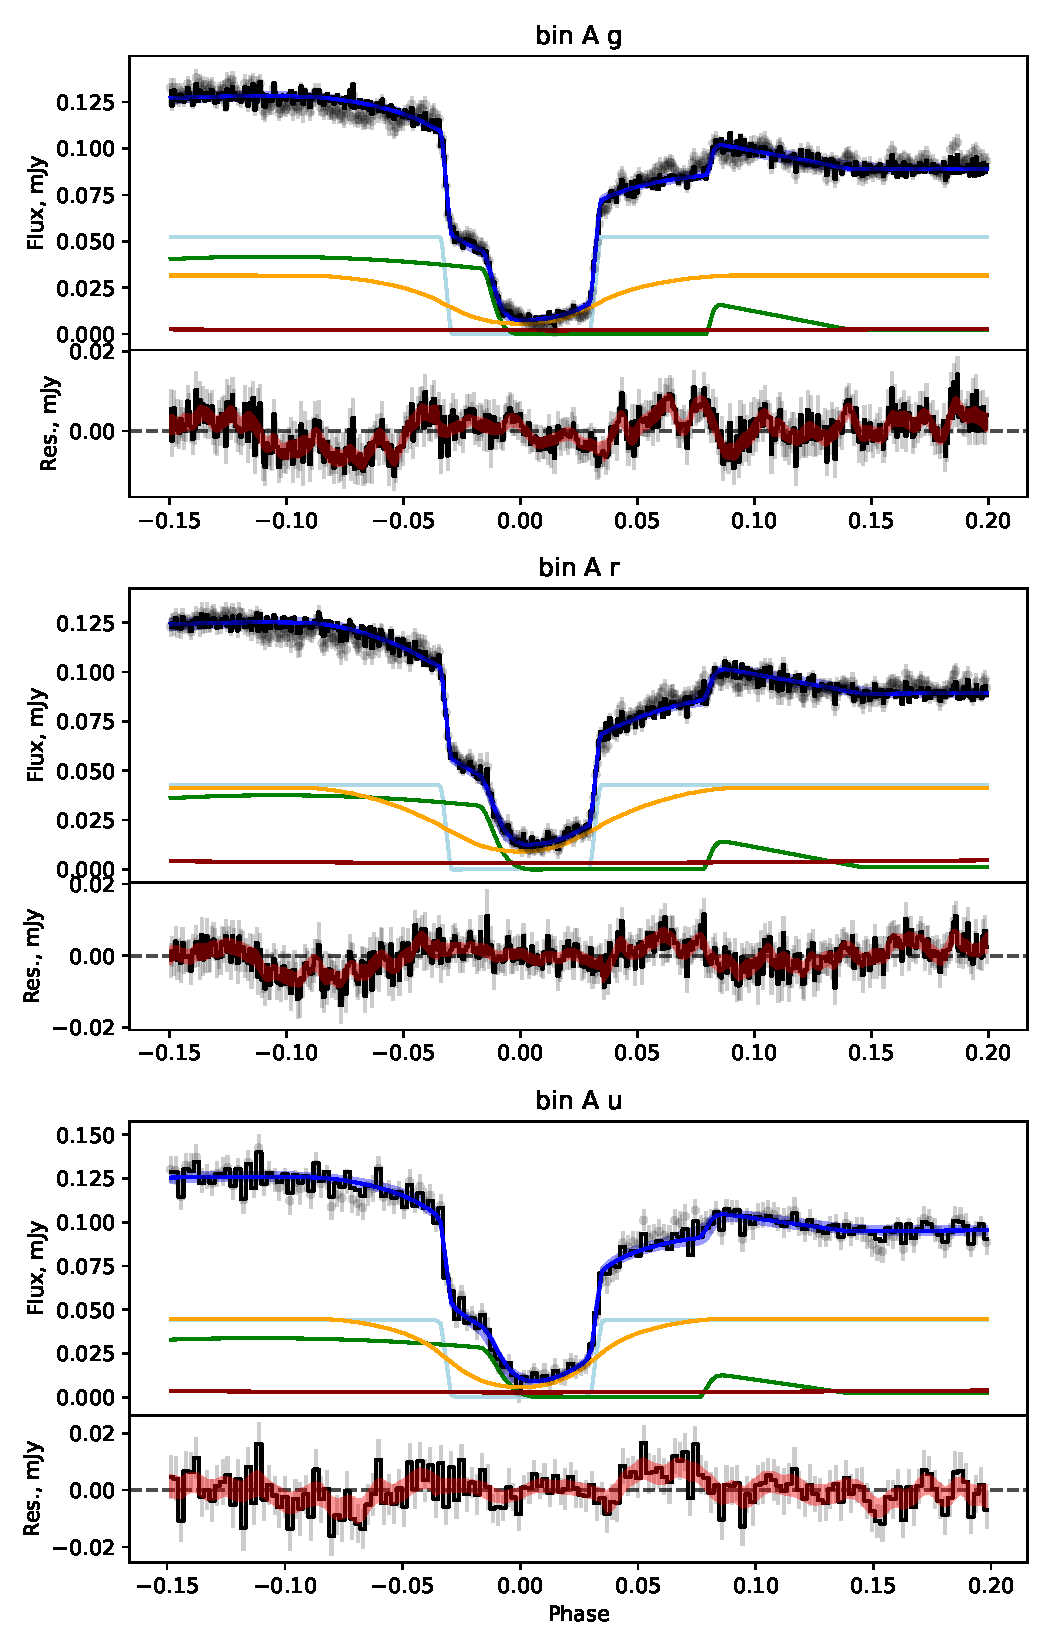
\includegraphics[width=\textwidth]{figures/results/MASOT0014/MASOT0014_3.pdf}
    \caption{MAS0014 lightcurve models (cont.)}
    \label{fig:MAS0014 all lightcurves cont 2}
\end{figure}



\section{White dwarf flux distributions, compared to cooling tracks}
\label{appendix:white dwarf fluxes}

\begin{figure}
    \centering
    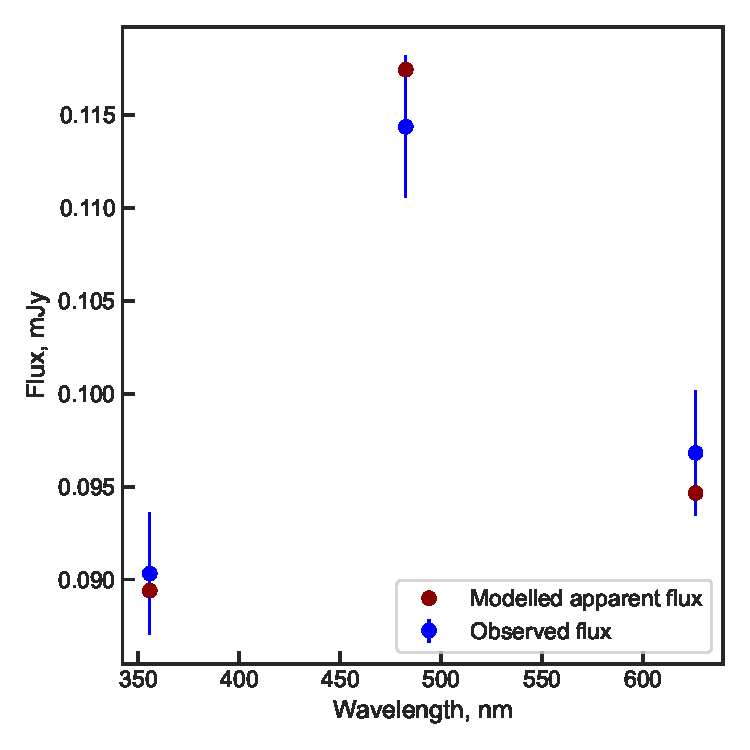
\includegraphics[width=\textwidth]{figures/results/ASASSN-14hq/fluxplot.pdf}
    \caption{ASASSN-14hq observed white dwarf fluxes, compared to the best-fit model atmosphere.}
    \label{fig:ASASSN-14hq flux plot}
\end{figure}

\begin{figure}
    \centering
    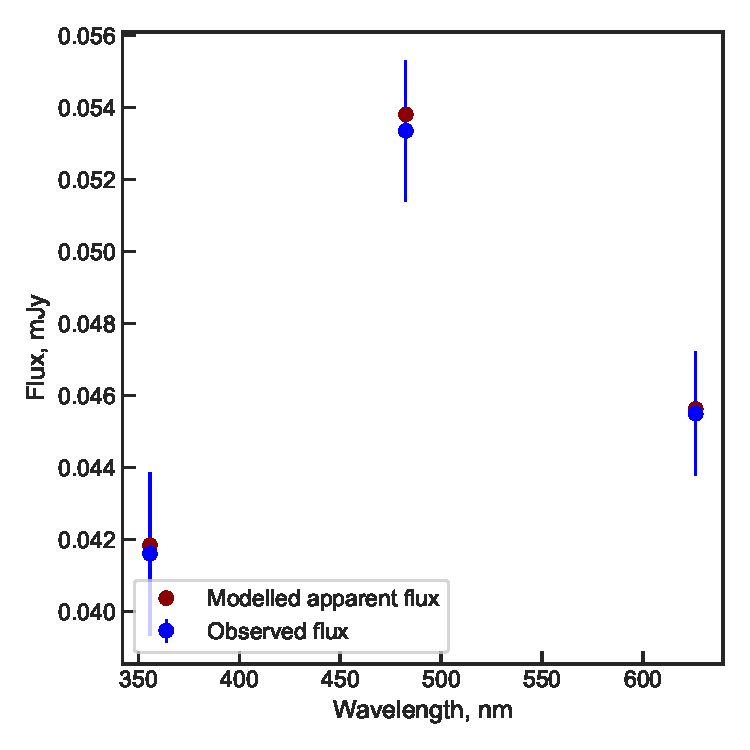
\includegraphics[width=\textwidth]{figures/results/ASASSN-14kb/fluxplot.pdf}
    \caption{ASASSN-14kb observed white dwarf fluxes, compared to the best-fit model atmosphere.}
    \label{fig:ASASSN-14kb flux plot}
\end{figure}

\begin{figure}
    \centering
    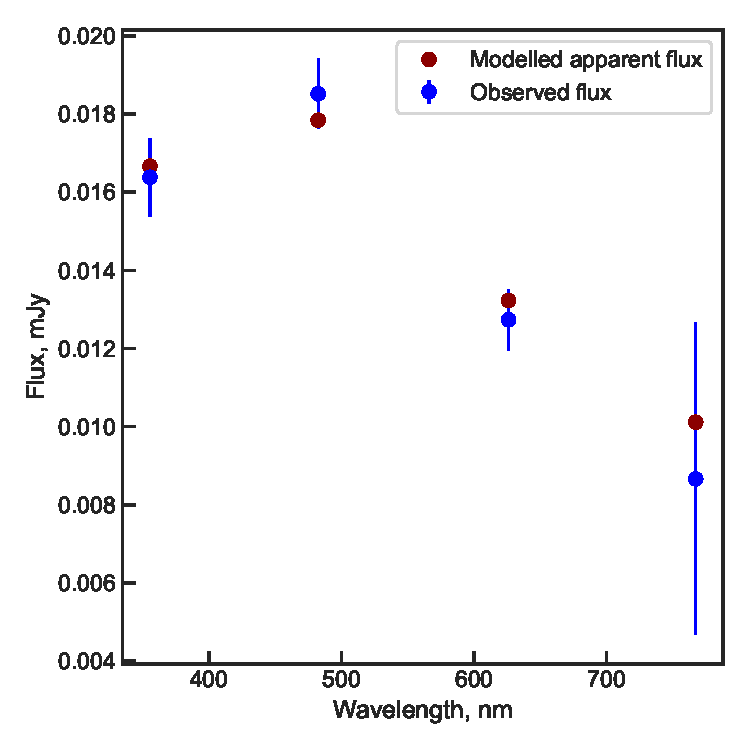
\includegraphics[width=\textwidth]{figures/results/ASASSN-15pb/fluxplot.pdf}
    \caption{ASASSN-15pb observed white dwarf fluxes, compared to the best-fit model atmosphere.}
    \label{fig:ASASSN-15pb flux plot}
\end{figure}

\begin{figure}
    \centering
    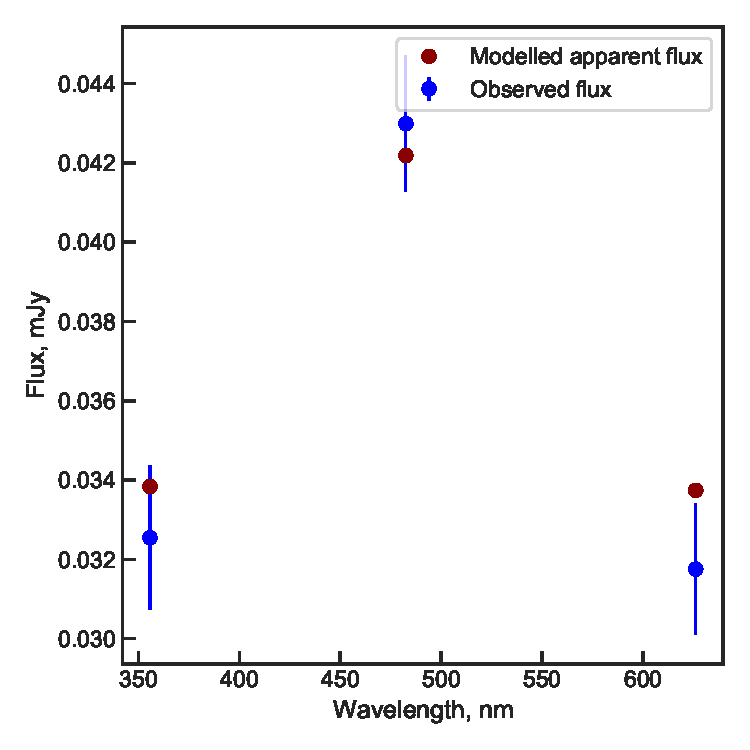
\includegraphics[width=\textwidth]{figures/results/ASASSN-17fo/fluxplot.pdf}
    \caption{ASASSN-17fo observed white dwarf fluxes, compared to the best-fit model atmosphere.}
    \label{fig:ASASSN-17fo flux plot}
\end{figure}

\begin{figure}
    \centering
    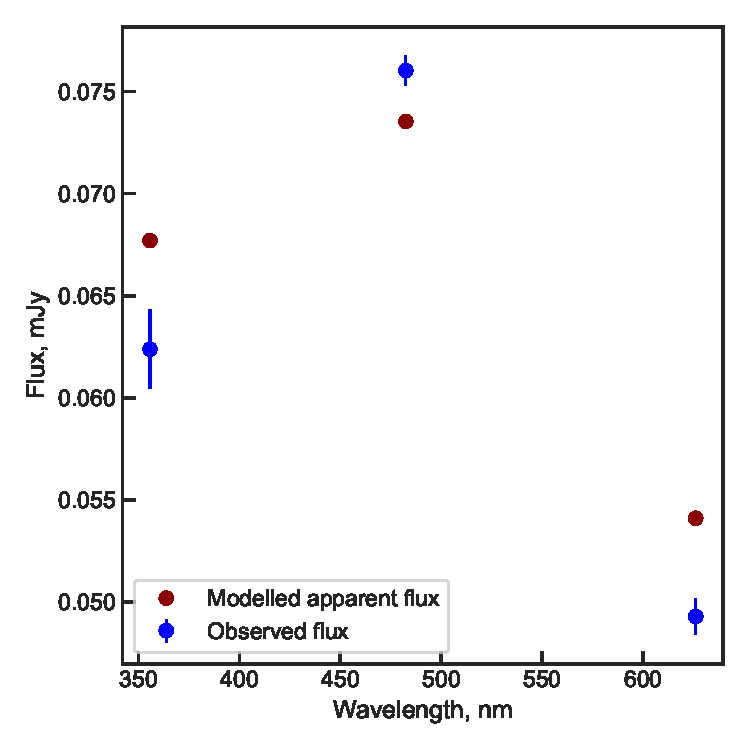
\includegraphics[width=\textwidth]{figures/results/AYFor/fluxplot.pdf}
    \caption{AY For observed white dwarf fluxes, compared to the best-fit model atmosphere.}
    \label{fig:AYFor flux plot}
\end{figure}

\begin{figure}
    \centering
    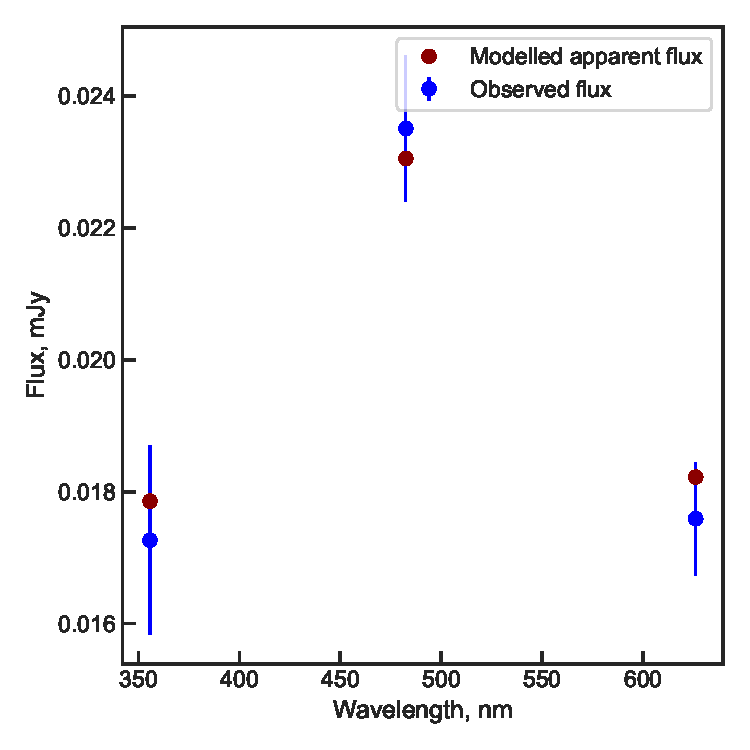
\includegraphics[width=\textwidth]{figures/results/CSS090102/fluxplot.pdf}
    \caption{CSS090102 observed white dwarf fluxes, compared to the best-fit model atmosphere.}
    \label{fig:CSS090102 flux plot}
\end{figure}

\begin{figure}
    \centering
    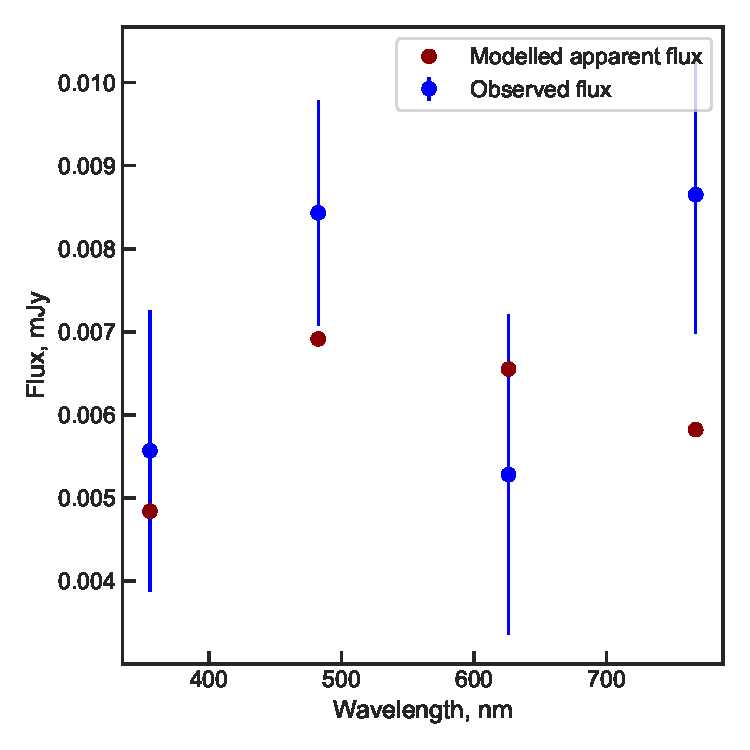
\includegraphics[width=\textwidth]{figures/results/CSS090419/fluxplot.pdf}
    \caption{CSS090419 observed white dwarf fluxes, compared to the best-fit model atmosphere.}
    \label{fig:CSS090419 flux plot}
\end{figure}

\begin{figure}
    \centering
    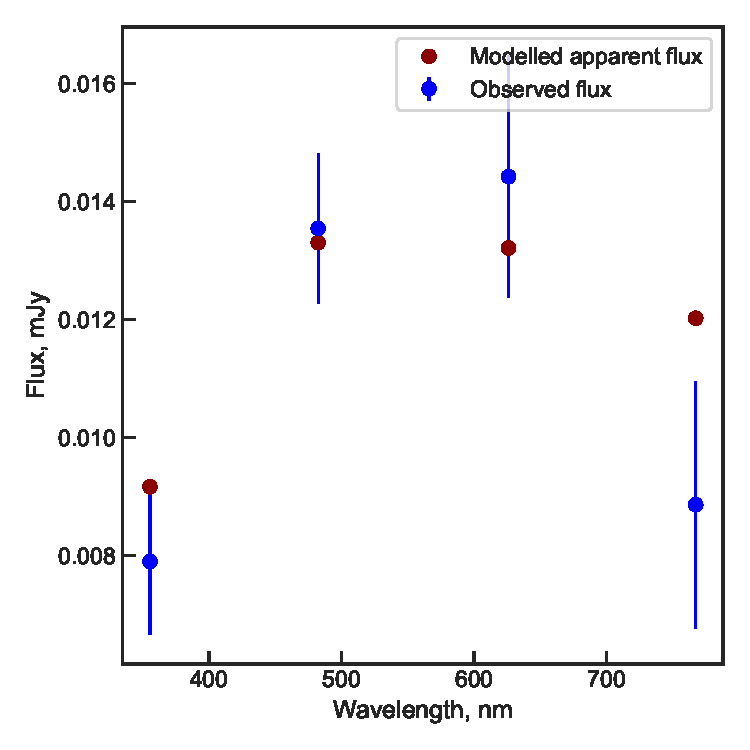
\includegraphics[width=\textwidth]{figures/results/CSS090622/fluxplot.pdf}
    \caption{CSS090622 observed white dwarf fluxes, compared to the best-fit model atmosphere.}
    \label{fig:CSS090622 flux plot}
\end{figure}

\begin{figure}
    \centering
    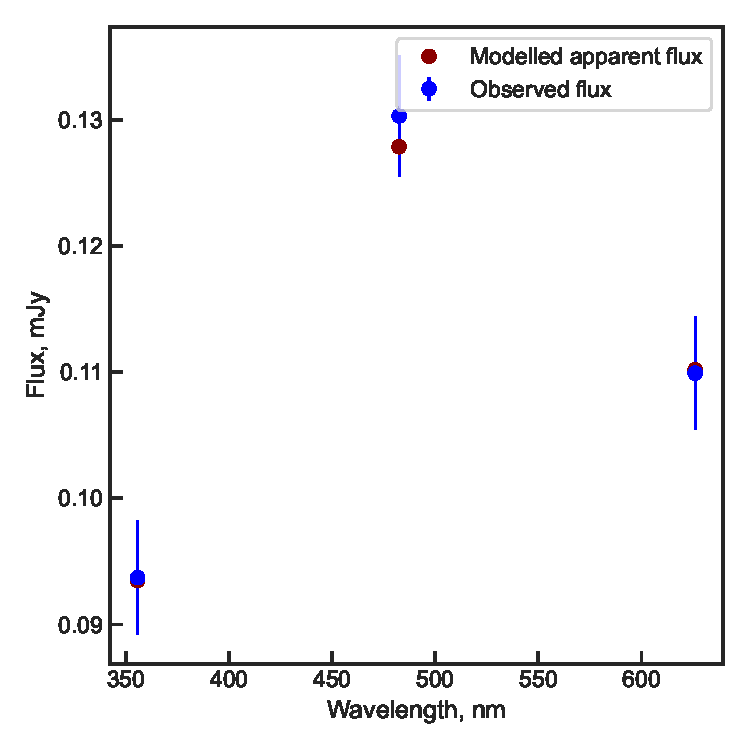
\includegraphics[width=\textwidth]{figures/results/OGLE82/fluxplot.pdf}
    \caption{OGLE82 observed white dwarf fluxes, compared to the best-fit model atmosphere.}
    \label{fig:OGLE82 flux plot}
\end{figure}

\begin{figure}
    \centering
    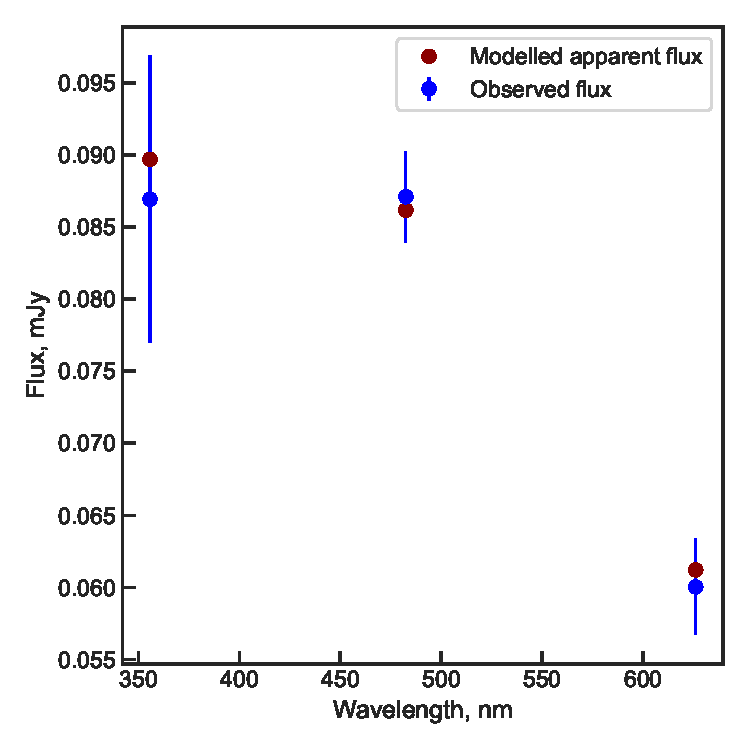
\includegraphics[width=\textwidth]{figures/results/SDSS0748/fluxplot.pdf}
    \caption{SDSS J0748 observed white dwarf fluxes, compared to the best-fit model atmosphere.}
    \label{fig:SDSS0748 flux plot}
\end{figure}

\begin{figure}
    \centering
    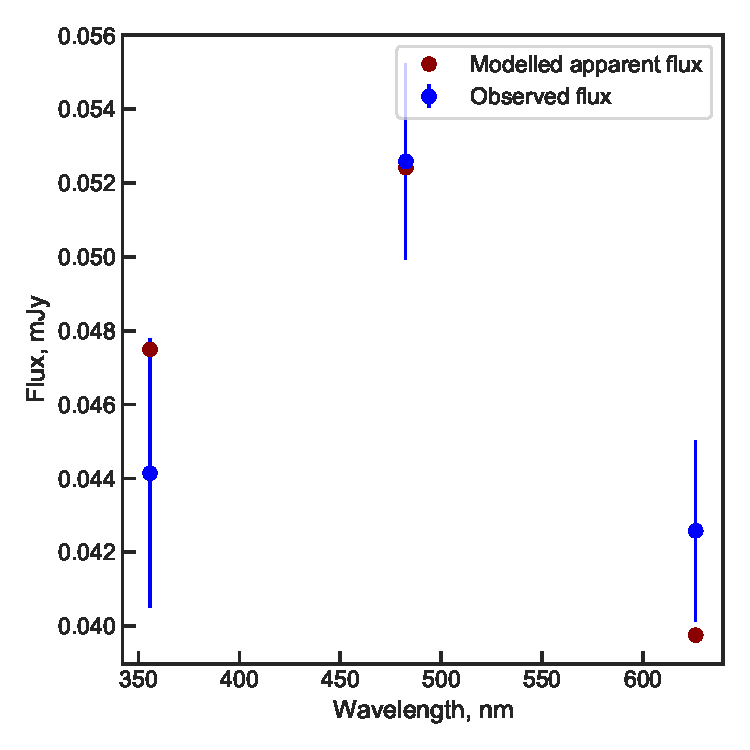
\includegraphics[width=\textwidth]{figures/results/MASOT0014/fluxplot.pdf}
    \caption{MAS0014 observed white dwarf fluxes, compared to the best-fit model atmosphere.}
    \label{fig:MAS0014 flux plot}
\end{figure}

% \begin{figure}
%     \centering
%     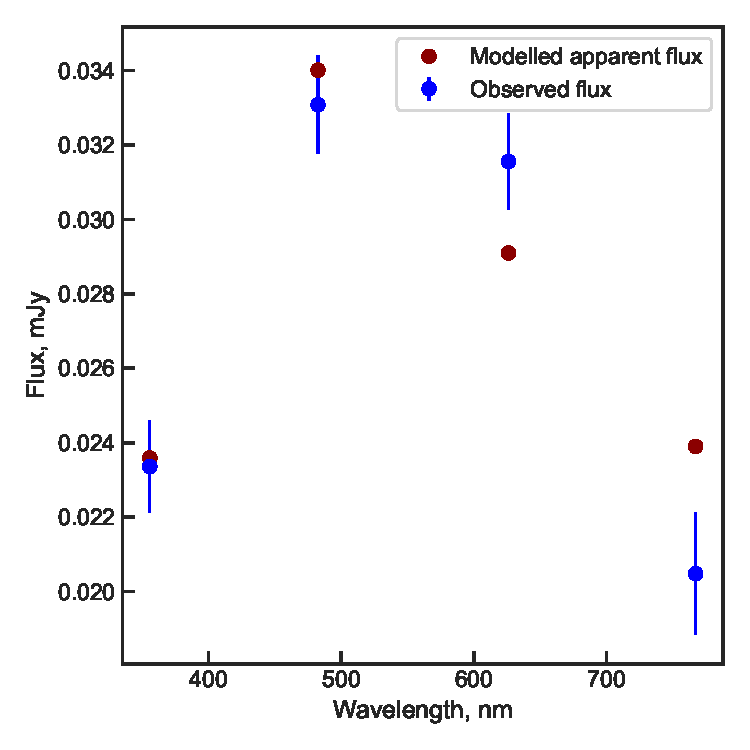
\includegraphics[width=\textwidth]{figures/results/SDSS1524/fluxplot.pdf}
%     \caption{SDSS1524 observed white dwarf fluxes, compared to the best-fit model atmosphere.}
%     \label{fig:SDSS1524 flux plot}
% \end{figure}



%%%%%%%%%%%%%%%%%%%%%%%%%%%%%%%%%%%%%%%%%%%%%%%%%%